\documentclass[10pt]{article}

\usepackage{array}
\usepackage{amsthm}
\usepackage{amsmath}
\usepackage{amssymb}
\usepackage{amsfonts}
\usepackage{stmaryrd}
\usepackage{tikz}
\usepackage{comment}
\usepackage{xspace}
\usepackage{makeidx}
\usepackage{stackengine}
\usepackage{ifthen}
\usepackage{listofitems}
\usepackage{graphicx}
\usepackage[final]{listings}
\usepackage{hyperref}
\usepackage{enumitem}

\graphicspath{ {.} }
\lstset{language=Java,
  commentstyle=\color{brown},
  keywordstyle=\color{blue},
  stringstyle=\color{red},
  basicstyle=\ttfamily}

\lstdefinelanguage{ddlog}{
  language=Java, % we base it on Java, just for comments
  morekeywords={input, output, typedef, relation, typedef, bool, not,
    string, bit, extern, function, var, for, match, skip, in, integer, % not really in DDlog
    Aggregate, FlatMap},
  deletestring=[b]{'}
}
\hypersetup{
  colorlinks   = true,    % Colours links instead of ugly boxes
  urlcolor     = blue,    % Colour for external hyperlinks
  linkcolor    = blue,    % Colour of internal links
  citecolor    = red      % Colour of citations
}
\hypersetup{final}

\usetikzlibrary{shapes, arrows.meta, positioning}
\tikzstyle{block} = [draw, fill=white, rectangle]

\newcommand{\rectangle}[5]{
\ifthenelse{\equal{#1}{1}}{
    \draw[fill=black!20!white] (#2,#3) rectangle(#4, #5);
}{
    \draw (#2,#3) rectangle(#4, #5);
}}

% A single box
\newcommand{\sngl}[1]{
\vcenter{\hbox{
\begin{tikzpicture}[scale=.4]
\rectangle{#1}{0}{0}{1}{1}
\end{tikzpicture}
}}}

% A column vector with two parts:
% a large one and a small one (last element)
% the two arguments are 0 for "empty" and 1 for "filled"
% they correspond to the two parts.  These must be used
% in math mode.
\newcommand{\strm}[1]{
\setsepchar{ }
\readlist\arg{#1}
\vcenter{\hbox{
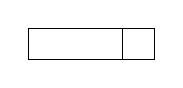
\begin{tikzpicture}[scale=.4]
\rectangle{\arg[1]}{0}{0}{3}{-1}
\rectangle{\arg[2]}{3}{0}{4}{-1}
\end{tikzpicture}
}}}

% A block matrix with 4 zones
\newcommand{\mtrx}[1]{
\setsepchar{ }
\readlist\arg{#1}
\vcenter{\hbox{

\begin{tikzpicture}[scale=.4]
\rectangle{\arg[1]}{0}{0}{3}{-3}
\rectangle{\arg[2]}{3}{0}{4}{-3}
\rectangle{\arg[3]}{0}{-3}{3}{-4}
\rectangle{\arg[4]}{3}{-3}{4}{-4}
\end{tikzpicture}
}}}

\newcommand{\matmult}[2]{\left( #1 \times #2 \right)}

\theoremstyle{definition}
\newtheorem{theorem}{Theorem}[section]
\newtheorem{lemma}[theorem]{Lemma}
\newtheorem{corollary}[theorem]{Corollary}
\newtheorem{definition}[theorem]{Definition}
\newtheorem{proposition}[theorem]{Proposition}
\newtheorem{example}[theorem]{Example}
\newtheorem{algorithm}[theorem]{Algorithm}

\newcommand{\secref}[1]{Section~\ref{#1}}  % reference to a section
\newcommand{\refsec}[1]{\secref{#1}}
% Used when a term is first defined.  Adds the term to the index.
\newcommand{\defined}[1]{\textbf{#1}\index{#1}}
\newcommand{\zr}{$\Z$-set\xspace}
\newcommand{\zrs}{$\Z$-sets\xspace} % plural
\newcommand{\means}[1]{\ensuremath{\llbracket #1 \rrbracket}}
\newcommand{\code}[1]{\mbox{\texttt{#1}}}
\newcommand{\Z}{\mathbb{Z}}  % integers
\newcommand{\R}{\mathbb{R}}  % reals
\newcommand{\N}{\mathbb{N}}  % naturals
\newcommand{\B}{\mathbb{B}}  % Booleans
\newcommand{\norm}[1]{\| #1 \|} % norm; requires math mode
% stream with elements of a given type
\newcommand{\stream}[1]{\ensuremath{\mathcal{S}_{#1}}}
% finite stream with elements of a given type (zero almost everywhere)
\newcommand{\streamf}[1]{\ensuremath{\overline{\mathcal{S}_{#1}}}}
\newcommand{\zm}{\ensuremath{z^{-1}}} % stream delay operator
\ifthenelse{\equal{1}{0}}{ % allows switching to mathit/mathcal
\newcommand{\I}{\mathcal{I}}  % stream integration
\newcommand{\D}{\mathcal{D}}  % stream derivative
}{
\newcommand{\I}{\mathit{I}}  % stream integration
\newcommand{\D}{\mathit{D}}  % stream derivative
}
\newcommand{\inc}[1]{{#1}^{\Delta}}
\newcommand{\dbsp}{DBSP\xspace}
\newcommand{\distinct}{\mathit{distinct}}  % distinct operator
% set with elements of given type
\newcommand{\set}[1]{\mathit{set}_{#1}}
\newcommand{\id}{\ensuremath{\mathit{id}}} % identity function
\newcommand{\isset}{\mbox{isset}}
\newcommand{\ispositive}{\mbox{ispositive}}
\newcommand{\defn}{\stackrel{\textrm{\scriptsize def}}{=}}
\newcommand{\map}{\mbox{map}}
\newcommand{\fix}[2]{\mbox{fix}\,#1.#2}
\newcommand{\lift}[1]{{\uparrow}#1}              
\newcommand{\rew}{\ensuremath{\mapsto}} % rewriting
\newcommand{\birew}{\ensuremath{\mapsfrom\!\mapsto}} % bidirectional rewriting
\newcommand{\pair}[2]{\ensuremath{\langle #1,#2 \rangle}} % pairing
\newcommand{\zpp}[1]{\mbox{zpp}(#1)}
\newcommand{\makeset}{\ensuremath{\mbox{makeset}}}
\newcommand{\sv}[1]{ % simple stream value, supplied as a space-separated list of 5 values
\setsepchar{ }
\readlist\arg{#1}
{[}
\begin{array}{cccccc}
    \arg[1] & \arg[2] & \arg[3] & \arg[4] & \arg[5] & \cdots
\end{array}
{]}
}

\newcommand{\st}{\;|\;}
\newcommand\Hookarrowleft[1]{\ensuremath{\stackrel{\curvearrowleft}{#1}}}

\newcommand{\cut}[2]{#1|_{_{\leq #2}}}
\newcommand{\scut}[2]{#1|_{_{< #2}}}


\setlength{\marginparwidth}{4cm}
\newcommand{\scream}[2]{\marginpar{\footnotesize \textbf{#1}: #2}}
\newcommand{\val}[1]{\scream{VAL}{#1}}
\newcommand{\mihai}[1]{\scream{MIHAI}{#1}}
\newcommand{\leonid}[1]{\scream{LEONID}{#1}}

\title{\dbsp: A Language for Expressing Incremental View Maintenance for Rich Query Languages}
\author{
Mihai Budiu \\ VMware Research \and 
Frank McSherry \\ Materialize Inc. \and 
Leonid Ryzhyk \\ VMware Research \and 
Val Tannen \\ University of Pennsylvania
}

\makeindex
\begin{document}

\maketitle

\url{https://www.overleaf.com/project/604c047e921769355e4a1a0f}

\begin{abstract}
Incremental view maintenance has been for a long time a central problem of database theory.
Many solutions have been proposed for restricted classes of database languages,
such as the relational algebra, or Datalog.  These techniques do not naturally generalize to
richer languages.  In this paper we give a general
solution to this problem in 3 steps: (1) we describe a simple but expressive language
called \dbsp for describing computations over data streams; (2) we give a general algorithm for 
solving the incremental view maintenance problem for arbitrary \dbsp programs, and (3) we show
how to model several classes of database query languages (including relational queries, 
grouping and aggregation, and recursion) using \dbsp.  \dbsp  
can be used to model other interesting query languages, including 
streaming aggregation queries, non-monotonic recursion, and queries on nested relations.  
As a consequence, we obtain efficient
incremental view maintenance techniques for all these rich languages.
\end{abstract}

\begin{quote}
This document is work in progress.  It contains a formal specification
of the \dbsp language, proofs of the theoretical results, and the
specification of the implementation of several query languages in
\dbsp.
\end{quote}

\tableofcontents

\section{Introduction}\label{sec:introduction}
%\tej{here's another attempt}

Incremental view maintenance (IVM) is an important and well-studied problem in
databases.  The IVM problem can be stated as follows: given a database $DB$ and
a view $V$ defined as a function of the database contents
(described by a query $Q$, i.e. $V = Q(DB)$),
maintain the contents of $V$ in response to changes of the database,
ideally more efficiently than by simply reevaluating $Q(DB)$ from scratch.  The goal is
to provide an algorithm that can evaluate $Q$ over the changes $\Delta DB$ applied
to the database, since in general the size of the changes is small $|\Delta DB| \ll |DB|$.

This paper provides a new perspective by proposing a new definition
of IVM based on a streaming model of computation\footnote{Our model is inspired by Digital Signal
Processing~\cite{rabiner-book75}, applied to databases, hence the name \dbsp.}.  Whereas previous
IVM solutions are based on defining a notion of a (partial) derivative of $Q$ with respect to its inputs,
our definition only requires computing \emph{derivatives of streams} as functions of time.
Derivatives of streams are always well-defined (assuming that the data computed on has a notion of difference
that satisfies some simple mathematical properties --- i.e., it forms a commutative
group.  Fortunately, it has long been known that relational databases can be modeled
in such a way, e.g.~\cite{green-pods07, koch-pods10}.)

\dbsp has several attractive properties:

\begin{enumerate}
\item is is \textbf{expressive}.  (a) It can be used to define
precisely multiple concepts: traditional queries, streaming computations, and incremental
computations.  (b) We have been able to express in \dbsp the full
relational algebra, computations over sets and bags,
nested relations, aggregation, flatmap, monotonic and nonmonotonic
recursion, stratified negation, while-relational programs, window queries,
streaming queries, streaming aggregation, and incremental versions of all
of the above.  In fact, we have built a \dbsp implementation of the
complete SQL language (\refsec{sec:implementation}).
\item it is \textbf{simple}.
\dbsp is built entirely on elementary concepts such as functions and algebraic groups.
\item mathematically \textbf{precise}.  All the results in this paper have been
formalized and checked using the Lean
proof assistant~\cite{moura-cade15}.
\item it is \textbf{modular}, in the following sense:
(a) the incremental version of a complex query can be reduced
recursively to incrementalizing its component subqueries.
This gives a simple, syntactic,
heuristic-free algorithm (Algorithm~\ref{algorithm-inc})
that converts an arbitrary \dbsp query to its incremental form.
(b) Extending \dbsp to support new primitive operators is easy,
and they immediately benefit from the rest of the theory of
incrementalization.
An important consequence of modularity is that the theory
can be efficiently implemented, as we
briefly discuss in \refsec{sec:implementation}.
\end{enumerate}

The core concept of \dbsp is the \emph{stream}, which is used to model changes
over time. We use $\stream{A}$ to denote the type of infinite streams with values of
type $A$. If $s \in \stream{A}$ is a stream,
then $s[t] \in A, t \in \mathbb{N}$ is the $t$th element of $s$, also referred to as the \emph{value of the stream at time $t$}.
A streaming computation is a function that
consumes one or more streams and produces another stream.  We show
streaming computations with diagrams, also called ``circuits'',
where boxes are computations and streams are arrows.  The following diagram
shows a stream operator $T: \stream{A} \times \stream{B} \to \stream{C}$,
consuming two input streams $s_0$ and $s_1$
and producing one output stream $s$:

\begin{center}
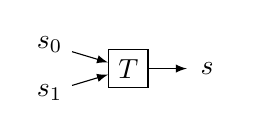
\begin{tikzpicture}[auto,>=latex,minimum width=.5cm]
  \node[] (input0) {$s_0$};
  \node[below of=input0,node distance=.3cm] (dummy) {};
  \node[below of=dummy,node distance=.3cm] (input1) {$s_1$};
  \node[block, right of=dummy] (T) {$T$};
  \node[right of=T] (output) {$s$};
  \draw[->] (input0) -- (T);
  \draw[->] (input1) -- (T);
  \draw[->] (T) -- (output);
\end{tikzpicture}
\vspace{-.2cm}
\end{center}

We generally think of streams as sequences of ``small'' values,
such as insertions or deletions in a database.
However, we also treat the whole database as a \emph{stream of database
snapshots}.  We model a database as a
stream $DB \in \stream{SCH}$, where $SCH$ is the database schema.
Time is not wall-clock time, but counts
the transactions applied to the database.
(Since transactions are linearizable, they have a total order.)
$DB[t]$ is the snapshot of the
database contents after $t$ transactions have been applied.

Database transactions also form a stream $\Delta DB$, this time a stream of \emph{changes},
or \emph{deltas} that are applied to the database.  The values of
this stream are defined by $(\Delta DB)[t] = DB[t] - DB[t-1]$, where ``$-$'' stands
for the difference between two databases, a notion that we will soon make more precise.
The $\Delta DB$ stream is produced from the $DB$ stream by
the \emph{stream differentiation} operator $\D : \stream{A} \to \stream{A}$;
this operator produces as its output the stream of changes from its input stream;
we have thus $\D(DB) = \Delta DB$.

Conversely, the database snapshot at time $t$ is the cumulative result of applying all
transactions up to $t$: $DB[t] = \sum_{i \leq t} \Delta DB[i]$.
The operation of adding up all changes is the inverse of differentiation,
and is another basic stream operator, \emph{stream integration}: $\I: \stream{A} \to \stream{A}$.
The following diagram expresses the relationship between the streams $\Delta DB$ and $DB$:

\begin{center}
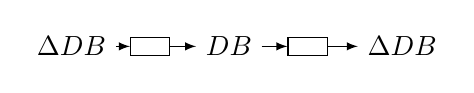
\begin{tikzpicture}[auto,>=latex,minimum width=.5cm]
  \node[] (input) {$\Delta DB$};
  \node[block, right of=input] (I) {$\I$};
  \node[right of=I] (output) {$DB$};
  \node[block, right of=output] (D) {$\D$};
  \node[right of=D, node distance=1.2cm] (end) {$\Delta DB$};
  \draw[->] (input) -- (I);
  \draw[->] (I) -- (output);
  \draw[->] (output) -- (D);
  \draw[->] (D) -- (end);
\end{tikzpicture}
\end{center}

Suppose we have a query $Q : SCH \to SCH$ defining a view $V$.  What is
a view in a streaming model?  It is also a stream!  For each snapshot
of the database stream we have a snapshot of the view: $V[t] = Q(DB[t])$.
In general, given an arbitrary function $f: A \to B$, we define
a streaming ``version'' of $f$, denoted by $\lift{f}$
(read as ``$f$ lifted''), which applies
$f$ to every element of the input stream independently.
We can thus write $V = (\lift{Q})(DB)$.

Armed with these basic definitions, we can now precisely define IVM.
What does it mean to maintain a view incrementally?  We claim that an
efficient maintenance algorithm needs to compute the \emph{changes} to
the view given the changes to the database.  We thus define the IVM of
a query $Q$ by chaining the above three definitions:
$\Delta V \defn \D(V) = \D(\lift{Q}(DB)) = \D(\lift{Q}(\I(\Delta DB)))$.
This can be shown as the following diagram, which is the central definition
of this paper:

\begin{center}
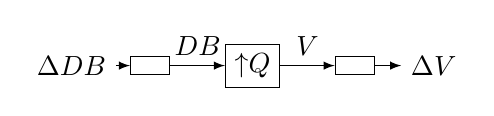
\begin{tikzpicture}[auto,>=latex,minimum width=.5cm]
  \node[] (input) {$\Delta DB$};
  \node[block, right of=input] (I) {$\I$};
  \node[block, right of=I, node distance=1.3cm] (Q) {$\lift{Q}$};
  \node[block, right of=Q, node distance=1.3cm] (D) {$\D$};
  \node[right of=D] (output) {$\Delta V$};
  \draw[->] (input) -- (I);
  \draw[->] (I) -- node (db) {$DB$} (Q);
  \draw[->] (Q) -- node (B) {$V$} (D);
  \draw[->] (D) -- (output);
\end{tikzpicture}
\end{center}

Given a query $Q$ we define its incremental version as
$\inc{Q} \defn \D \circ \lift Q \circ \I$.  The incremental version
of a query is a \emph{streaming operator} which computes directly on changes
and produces changes.  The incremental version of a query is thus always
well-defined.  The above definition shows one way to compute a query
incrementally, but applying it naively will generally produce an inefficient
execution plan, since it will reconstruct the database at each step.  In \refsec{sec:incremental}
we show how algebraic properties of the $\inc{\cdot}$ transformation can be used to
optimize the implementation of $\inc{Q}$. The first key property is that the
composition of queries can be incrementalized by composing the incremental
versions of its constituents, that is
$\inc{(Q_1 \circ Q_2)} = \inc{Q_1} \circ \inc{Q_2}$.  The second key
property is that essentially all primitive database operations have efficient incremental
versions.

Armed with this general theory of incremental computation, in \secref{sec:relational}
we show how to model relational queries in \dbsp.  This immediately gives
us a general algorithm to compute the incremental version of any relational query.
These results were previously known, but they are cleanly modeled by \dbsp.
\secref{sec:datalog} shows how recursive Datalog
programs with stratified negation can be implemented in \dbsp, and \secref{sec:nested} gives
\emph{incremental streaming computations for recursive programs}. For example, given an implementation of
transitive closure in the natural recursive way, our algorithm produces a program that efficiently maintains the
transitive closure of a graph as the graph is changed by adding and deleting edges.

We have formalized the entire \dbsp theory in the Lean proof
assistant~\mihai{Need a URL for this}; our formalization
includes machine-checked proofs of correctness for all the theorems
stated in this paper.

This paper makes the following contributions:
\begin{enumerate}
  \item \dbsp, a \textbf{simple} but \textbf{expressive} language for streaming
  computation. \dbsp gives an elegant formal foundation unifying the manipulation of
  streaming and incremental computations.
  \item An algorithm for incrementalizing any streaming computation expressed in
  \dbsp.
  \item An illustration of how \dbsp can be applied to various query classes, such as relational algebra,
  nested relations, aggregations, flatmap, and stratified-monotonic Datalog.
  \item We offer the first fully mechanically-verified theory of IVM.
  \item We provide a high-performance open-source implementation of DBSP as a
  general-purpose streaming query engine in Rust.
\end{enumerate}

The following tables summarize the mathematical notations used in the rest of this paper.

\noindent
\begin{center}
\begin{tabular}{|c|p{10cm}|} \hline
%\textbf{Notation} & \textbf{Meaning} \\ \hline

\multicolumn{2}{|c|}{General notations} \\ \hline
$\Z$ & The ring of integer numbers \\
$\N$ & The set of natural numbers $0, 1, 2, \ldots$ \\
$\B$ & The set of Boolean values \\
$[n]$ & The natural numbers between 0 and $n-1$ \\
$\id$ & The identity function over some domain $\id: A \to A$, $\id(x) = x$ \\
$\means{Q}$ & Semantics of query (function) $Q$ \\
$\pair{a}{b}$ & The pair containing values $a$ and $b$ \\
fst$(p)$ & The operator that returns the first value of a pair $p$ \\
snd$(p)$ & The operator that returns the second value of a pair $p$ \\
$a \mapsto b$ & The function that maps $a$ to $b$ and everything else to 0 \\
$\lambda x.M$ & An anonymous function with argument $x$ and body $M$ \\
$\fix{x}{f}$ & The (unique) solution (fixed point) of the equation $f(x) = x$ \\
\hline
\end{tabular}

\noindent
\begin{tabular}{|c|p{10cm}|} \hline
\multicolumn{2}{|c|}{Streams} \\ \hline
$\stream{A}$ & The set of streams with elements from a group $A$; $\stream{A} = \{ f \,|\, f : \N \to A \}$ \\
$\streamf{A}$ & Streams with elements from a group $A$ that are 0 almost everywhere \\
$s[t]$ & The $t$-th element of a stream; $s[t] = s(t)$ \\
$\lift{f}$ & An operator applied to a function $f: A \to B$ to produce a function $\lift{f}: \stream{A} \to \stream{B}$
           operating pointwise \\
$\zpp{f}$ & $\zpp{f}$ iff $f(0) = 0$ for $f: A \to B$ for $A, B$ groups \\
$\zm$ & The stream delay operator $\zm: \stream{A} \to \stream{A}$, that outputs a 0 followed by the input stream \\
$\I$ & The stream integration operator $\I: \stream{A} \to \stream{A}$ \\
$\D$ & The stream differentiation operator $\D: \stream{A} \to \stream{A}$ \\
$\inc{Q}$ & The incremental version of an operator $\inc{Q} = \D \circ Q \circ \I$ \\
$\cut{s}{t}$ & A stream that has the same prefix as $s$ up to $t$, then it is all 0s \\
$\scut{s}{t}$ & A stream that has the same prefix as $s$ up to $t-1$, then it is all 0s \\
$\cong$ & Symbol that indicates that two circuits compute the same function \\
$\delta_0$ & A function that produces a stream from a scalar: scalar, followed by zeros \\
$\int$ & A function that produces a scalar by adding all elements of a stream \\
$E$ & $E = \I \circ \delta_o$ \\
$X$ & $X = \int \circ \D$ \\
\hline
\multicolumn{2}{|c|}{\zrs} \\ \hline
$\Z[A]$ & \zrs: finite functions from $A \to \Z$ \\
$DB$ & A database \\
$\Delta DB$ & A change to a database \\
$|s|$ & Size of \zr $s$ \\
$\isset$ & A function $\isset: \Z[A] \to \B$ that determines whether its argument is a set \\
$\distinct$ & A function $\distinct: \Z[A] \to \Z[A]$ that always returns a set \\
$\ispositive$ & A function $\ispositive: \Z[A] \to \B$ that determines whether all elements of a \zr have positive weights \\
toszet & Function converting a set to a \zr \\
toset & Function converting a \zr into a set \\
\hline
\end{tabular}
\end{center}

\section{Related work}\label{sec:related}

\subsection{Incremental View Maintenance}

Incremental view maintenance~\cite{gupta-sigmod93, griffin-sigmod95, chaudhuri-icde95,
gupta-idb95, chirkova-book12} is a much studied problem in databases.
A survey of results for Datalog queries is present in~\cite{motik-ai19}.
The standard approach is as follows: given a query $Q$, discover a ``delta query'',
a``differential'' version $\Delta Q$ that satisfies the equation:
$Q(d+\Delta d)=Q(d)+\Delta Q(d,\Delta d)$, and which can be used to compute
the change for a new input reusing the previous output.
DBToaster introduced recursive recursive IVM~\cite{ahmad-vldb09, koch-pods10}, where
the incrementalization process is repeated for the delta query.

Many custom algorithms were published for various classes of queries: e.g.~\cite{koch-pods16}
handles positive nested relational calculus.  DYN~\cite{idris-sigmod17}
and IDYN~\cite{idris-vldb18, idris-sigmod19} focus on acyclic conjunctive queries.  Instead
of keeping the output view materialized they build data structures that allow efficiently
querying the output views.  PAI maps~\cite{abeysinghe-sigmod22} are specially
designed for queries with correlated aggregations.
AJU~\cite{wang-sigmod20} focuses on foreign-key joins.  It is a matter
of future work to evaluate whether custom \dbsp operators
can match the efficiency of systems specialized for narrow classes
of queries.

\dbsp is a bottom-up system, which always produces eagerly
the\emph{changes} to the output views.
Instead of maintaining the output view entirely, \dbsp proposes
generating deltas as the output of the computation (similar to the kSQL~\cite{jafarpour-edbt19}
\texttt{EMIT CHANGES} queries).  The idea that both
inputs and outputs to an IVM system are streams of changes
seems trivial, but this is key to the symmetry of our solution:
both in our definition of IVM~(\ref{def:inc}), and the fundamental
reason that the chain rule exists --- the chain rule is the one that makes our
structural induction IVM algorithm possible.

IVM algorithms for Datalog-like languages frequently use counting based
approaches~\cite{Dewan-iis92,motik-aaai15} that maintain the number of derivations of each
output fact: DRed~\cite{gupta-sigmod93} and its variants~\cite{Ceri-VLDB91,Wolfson-sigmod91,%
Staudt-vldb96,Kotowski-rr11,Lu-sigmod95,Apt-sigmod87}, the backward-forward algorithm
and variants~\cite{motik-aaai15,Harrison-wdd92,motik-ai19}.
\dbsp is more general than these approaches,
and our incrementalization algorithm handles arbitrary recursive queries and
generates more efficient plans for recursive queries
in the presence of arbitrary updates (especially deletions, where competing approaches
may over-delete).  Interestingly, the \zrs multiplicities in \dbsp are related
to the counting-number-of-derivations approaches, but our use of the $\distinct$
operator shows that precise counting is not necessary.

Picallo et al.~\cite{picallo-scop19} provide a general solution to IVM for
rich languages.  \dbsp requires a group structure on the values operated on;
this assumption has two major practical benefits: it simplifies the mathematics considerably
(e.g., Picallo uses monoid actions to model changes), and it provides a general, simple
algorithm (\ref{algorithm-inc}) for incrementalizing arbitrary programs.  The downside of
\dbsp is that one has to find a suitable group structure (e.g., \zrs for sets) to ``embed''
the computation.  Picallo's notion of ``derivative'' is not unique: they need creativity to choose
the right derivative definition, we need creativity to find the right group structure.

Finding a suitable group structure has proven easy for relations (both~\cite{koch-pods10}
and~\cite{green-tcs11} use \zrs to uniformly model data and insertions/deletions), but it is
not obvious how to do it for other data types, such as sorted collections, or tree-shaped
collections (e.g., XML or JSON documents)~\cite{foster-planx08}.  An intriguing question
is ``what other interesting group structures could this be applied to besides \zrs?''
Papers such as~\cite{nikolic-icmd18} explore other possibilities, such as matrix algebra,
linear ML models, or conjunctive queries.

\dbsp does not do anything special for triangle queries~\cite{kara-tds20}.  Are there
better algorithms for this case?

In \secref{sec:extensions} we have briefly mentioned that \dbsp can easily
model window and stream database queries~\cite{arasu-tr02,aurora}; it is an
interesting question whether there are CQL queries that cannot be expressed in \dbsp
(we conjecture that there aren't any).

\begin{comment}
The main problem that change structures address is that the types used in programs are not
closed under subtraction (e.g., the delta between two sets is not a set).
Although a relational \dbsp circuit computes
only on positive \zr values, its incremental version may compute on negative
values, but the equivalence of the two programs guarantees correctness even though the
type system of \zrs does not.  \val{Safe to delete this para}
\end{comment}


\dbsp is also related to Differential Dataflow
(DD)~\cite{mcsherry-cidr13, murray-sosp13} and its theoretical
foundations~\cite{abadi-fossacs15} (and
recently~\cite{mchserry-vldb20,chothia-vldb16}).  DD's computational
model is more powerful than \dbsp, since it allows past values in a
stream to be "updated".  In fact, DD is the only other framework which
we are aware of which can incrementalize recursive queries as
efficiently as \dbsp does.  In contrast, our model assumes that the
inputs of a computation arrive in the time order while allowing for
nested time domains via the modular lifting transformer ($\lift{}$).
\dbsp can express both incremental and non-incremental computations;
in essence \dbsp is ``deconstructing'' DD into simple component
building blocks.  Most importantly, \dbsp comes with
Algorithm~\ref{algorithm-inc}, a syntax-directed translation that can
convert any expressible query into an incremental version --- in DD
users have to assemble incremental queries manually using incremental
operators.  (materialize.com offers a product that automates
incrementalization, but only for SQL queries.  Differential
Datalog~\cite{ryzhyk-datalog19} does it for a Datalog dialect.)
Unlike DD, \dbsp is a modular theory, which easily accommodates the
addition of new operators.  In particular, we have given full
mechanical proofs of \dbsp's correctness.

\subsection{Stream computation models}

\dbsp using non-nested streams is a simplified instance of a Kahn
network~\cite{kahn-ifip74}.  Johnson~\cite{johnson-phd83} studies a
very similar computational model without nested streams and its
expressiveness. The implementation of such streaming models of
computation and their relationship to dataflow machines has been
studied by Lee~\cite{lee-ieee95}.  Lee~\cite{lee-ifip93} also
introduced streams of streams and the $\lift{\zm}$ operator.

\cite{gammie-acs13} surveys the connection between synchronous digital
circuits and functional programs.  Our circuits are nothing but higher
order functions computing on streams (functions themselves).  The
paper's main focus are circuits processing numeric data, whereas,
taking advantage of our circuits' ability to compute on arbitrary
groups, we use circuits to implement incremental view maintenance for
relational databases.

Mamouras~\cite{mamouras-esop20} gives a formal theory of stream computation.

\subsection{Connection to synchronous circuits}

There is a vast literature on \defined{synchronous circuits}, which
are well-defined models for hardware circuits
e.g.~\cite{gammie-acs13}.  These circuits also compute over infinite
streams of values, usually of Booleans $\stream{\B}$.  In a
\defined{combinational circuit} the output values depend only on the
current input values.  These are pure lifted streaming computations.
A \defined{sequential circuit} can have outputs that depend on past
input values.  These are always causal circuits.  Sequential
synchronous circuits use latches or flip-flops to store state; the
latches are controlled by a global clock signal.  These correspond to
the $\zm$ operator.  In a well-formed sequential circuit all
back-edges must go through some latch --- this corresponds to our
circuit construction rule that requires a delay element on each
back-edge.

Languages such as Verilog or VHDL can be used to specify such
circuits.  (However, both Verilog and VHDL are strictly more powerful,
and can express richer classes of circuits than just synchronous
sequential circuits.)

There is a rich literature on synchronous circuits, and some of these
results are directly applicable to the circuits we discuss.  Here are
a few examples.

Retiming~\cite{leiserson-algorithmica91} is an optimization that
``moves'' around delay elements while preserving the circuit
semantics.  Retiming is used traditionally to reduce the clock cycle
by minimizing the signal propagation delay between any pair of
latches.  In our case it could be used for minimizing the amount of
internal circuit state.

In a synchronous circuit the \emph{state} is entirely stored in the
latches.  Saving and restoring the contents of the latches enables
such circuits to take a snapshot of their state and resume
computation.\footnote{In Boolean synchronous circuits this is achieved
  by connecting all latches into a \emph{scan chain} which can be read
  and written sequentially after stopping the circuit clock.}

Fault tolerance of synchronous circuits is provided by replicating the
state elements, to prevent accidental state changes caused by e.g.,
cosmic rays.  We can borrow this idea for building redundant
distributed computations.

Pipelining digital circuits is an effective technique for increasing
throughput through parallelization, by inserting additional latches
and allowing different pipeline stages to compute concurrently on
distinct stream values, at the expense of increased latency between
the inputs and the corresponding outputs.

Digital circuit latches depend on a special ``reset'' signal to
initialize their state to a pre-established value; this corresponds to
the special 0 value in our value domain.

Our nested streams are related to the notion of delta-cycles in the
definition of VHDL~\cite{baker-date96}.


\part{Streaming and incremental computations}
\section{Stream computations}\label{sec:streams}

The core notion of our theory of IVM is the \textbf{stream}.
In this section we introduce formally streams as
infinite sequences of values, and define computations on streams.
Stream operators (\secref{sec:notation}) are the basic building block of stream
computations.  Operators can be composed with simple rules (\secref{sec:abelian})
into complex computational circuits.
In (\secref{sec:abelianstreams}) we introduce two essential operations on streams:
integration and differentiation.

\subsection{Streams and stream operators}\label{sec:notation}

$\N$ is the set of natural numbers (from 0), $\B$ is the set of
Booleans, $\Z$ is the set of integers, and $\R$ is the set of real
numbers.

\begin{definition}[stream]
Given a set $A$, a \defined{stream} \emph{of values from $A$}, or an
\emph{$A$-stream}, is a function $\N \rightarrow A$.  We denote by
$\stream{A} \defn \{ s \,|\, s : \N \to A \}$ the set of all
$A$-streams.
\end{definition}

When $s\in\stream{A}$ and $t\in\N$ we
write $s[t]$ for the $t$-th element of the stream $s$ instead of the usual $s(t)$.
We think of the index $t\in\N$ as (discrete) time and of $s[t]\in A$
as the value of the the stream $s$ ``at time'' $t$.
\ifstreamexamples
For example, the stream of natural numbers $id \in \stream{\N}$ given by $\id[t] = t$ is the sequence of values
$\sv{0 1 2 3 4}$.
\fi

\begin{definition}[stream operator]
A \defined{stream operator} with $n$ inputs is a function
$T:\stream{A_0}\times\cdots\times\stream{A_{n-1}}\to\stream{B}$.
\end{definition}
In general we use ``operator'' for functions on streams, and
``function'' for computations on ``scalar'' values.

\dbsp is an extension of the simply-typed lambda calculus ---
we will introduce its elements gradually.  However, in many cases we find it more readable to
use circuit diagrams to depict \dbsp programs.
(Circuits do hide the \emph{order} of the inputs of an operator; for non-commutative
operators we have to distinguish the operator inputs.)
In a circuit a rectangle represents an operator application (labeled
with the operator name, e.g., $T$), while an arrow is a stream.

Stream operator \emph{composition} (function composition) is shown as chained circuits.
The composition of a binary operator $T: \stream{A} \times \stream{B} \to \stream{A}$ with the
unary operator $S: \stream{A} \to \stream{B}$ into the computation
$\lambda s. T(T(s,S(s)),S(s)) : \stream{A}\to\stream{A}$
is:

\begin{center}
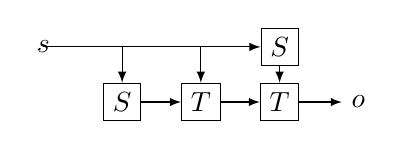
\begin{tikzpicture}[auto,>=latex]
  \node[] (input) {$s$};
  \node[] [right of=input] (dummy) {};
  \node[block, below of=dummy, node distance=.7cm] (S1) {$S$};
  \node[block, right of=S1] (T1) {$T$};
  \node[block, right of=T1] (T2) {$T$};
  \node[block, above of=T2, node distance=.7cm] (S2) {$S$};
  \node[right of=T2] (output) {$o$};
  \draw[->] (input) -| (S1);
  \draw[->] (input) -| (T1);
  \draw[->] (S1) -- (T1);
  \draw[->] (T1) -- (T2);
  \draw[->] (input) |- (S2);  \draw[->] (T2) -- (output);
  \draw[->] (S2) -- (T2);
\end{tikzpicture}
\end{center}


\begin{definition}(lifting)
Given a (scalar) function $f: A \to B$,
we define a stream operator $\lift{f} :\stream{A} \to \stream{B}$
by \emph{lifting} the function $f$ pointwise in time: $(\lift{f})(s) \defn f \circ s$.
Equivalently, $((\lift{f})(s))[t] \defn f(s[t])$.
This extends to functions of multiple arguments.
\end{definition}

\ifstreamexamples
For example, $(\lift{(\lambda x.(2x))})(id) = \sv{0 2 4 6 8}$.
\fi

\begin{proposition}[distributivity]\label{prop:distributivity}
Lifting distributes over function composition:
$\lift{(f \circ g)} = (\lift{f}) \circ (\lift{g})$.
\end{proposition}
\begin{comment}
\begin{proof}
This is easily proved by using associativity of function composition:
$\forall s . (\lift{(f \circ g)})(s) = (f \circ g) \circ s =
f \circ (g \circ s) = f \circ (\lift{g})(s) = (\lift{f})((\lift{g})(s)) =
(\lift{f} \circ \lift{g})(s).$
\end{proof}
\end{comment}

We say that two \dbsp programs are \defined{equivalent} if they compute the same
input-output function on streams.
We use the symbol $\cong$ to indicate that two circuits are
equivalent.  For example, Proposition~\ref{prop:distributivity}
states the following circuit equivalence:

\noindent
\begin{tabular}{m{3.5cm}m{.3cm}m{3.5cm}}
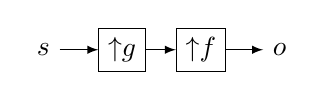
\begin{tikzpicture}[auto,>=latex]
  \node[] (input) {$s$};
  \node[block, right of=input] (g) {$\lift{g}$};
  \node[block, right of=g] (f) {$\lift{f}$};
  \node[right of=f] (output) {$o$};
  \draw[->] (input) -- (g);
  \draw[->] (g) -- (f);
  \draw[->] (f) -- (output);
\end{tikzpicture}
&
$\cong$
&
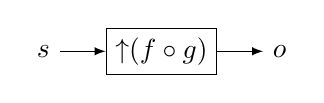
\begin{tikzpicture}[auto,>=latex]
    \node[] (input) {$s$};
    \node[block, right of=input, node distance=1.5cm] (fg) {$\lift{(f \circ g)}$};
    \node[right of=fg, node distance=1.5cm] (output) {$o$};
    \draw[->] (input) -- (fg);
    \draw[->] (fg) -- (output);
\end{tikzpicture}
\end{tabular}

\subsection{Streams over abelian groups}\label{sec:abelian}

For the rest of the technical development we require the set of values
$A$ of a stream $\stream{A}$ to form a commutative group $(A, +, 0_A,
-)$.  The plus defines what it means to add new data, while the minus
allows us to compute differences (deltas); the group structure will
allow us to reorder insertions and deletions.  We show later that this
restriction is not a problem for using \dbsp with relational data.
Now we introduce some useful operators and study their properties.

\subsubsection{Delays and time-invariance}\label{sec:delay}

\begin{definition}[Delay]
The \defined{delay operator}\footnote{The name $\zm$
comes from the DSP literature, and is related to the z-transform~\cite{rabiner-book75}.}
produces an output stream
by delaying its input by one step: $\zm_A: \stream{A} \to \stream{A}$:
%\begin{tabular}{m{5cm}m{3cm}}
$$
\zm_A(s)[t] \defn   \begin{cases}
0_A      & \text{when}~t=0 \\
s[t - 1] & \text{when}~t\geq1
\end{cases}
$$
%&
%\begin{tikzpicture}[auto,node distance=1cm,>=latex]
%    \node[] (input) {$s$};
%    \node[block, right of=input] (z) {$\zm$};
%    \node[right of=z] (output) {$o$};
%    \draw[->] (input) -- (z);
%    \draw[->] (z) -- (output);
%\end{tikzpicture}
%\end{tabular}
\end{definition}

We often omit the type parameter $A$, and write just $\zm$.
\ifstreamexamples
For example, $\zm(\id) = \sv{0 0 1 2 3}$.
\fi

\begin{definition}[Time invariance]
A stream operator $S: \stream{A} \to \stream{B}$ is \defined{time-invariant} (TI) if
$S(\zm_A(s)) = \zm_B(S(s))$ for all $s \in \stream{A}$; in other words, the
if following two circuits are equivalent:

\begin{tabular}{m{3cm}m{.5cm}m{3cm}}
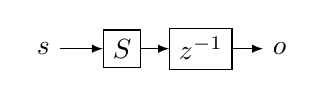
\begin{tikzpicture}[auto,>=latex]
  \node[] (input) {$s$};
  \node[block, right of=input] (S) {$S$};
  \node[block, right of=S] (z) {$\zm$};
  \node[right of=z] (output) {$o$};
  \draw[->] (input) -- (S);
  \draw[->] (S) -- (z);
  \draw[->] (z) -- (output);
\end{tikzpicture}
&
$\cong$
&
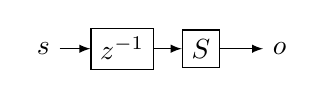
\begin{tikzpicture}[auto,>=latex]
  \node[] (input) {$s$};
  \node[block, right of=input] (z) {$\zm$};
  \node[block, right of=z] (S) {$S$};
  \node[right of=S] (output) {$o$};
  \draw[->] (input) -- (z);
  \draw[->] (z) -- (S);
  \draw[->] (S) -- (output);
\end{tikzpicture}
\end{tabular}

\noindent
This definition extends
naturally to operators with multiple inputs.
\end{definition}

The composition of TI operators of any number of inputs
is TI. The delay operator $\zm$ is TI.
\dbsp only uses TI operators.

%\begin{definition}
%We say that a function between groups $f: A \to B$ has the \emph{zero-preservation
%property} if $f(0_A) = 0_B$.  We write $\zpp{f}$.
%\end{definition}
%
%A lifted operator $\lift{f}$ is TI iff $\zpp{f}$.

\subsubsection{Causal and strict operators}\label{sec:causal}

\begin{definition}[Causality]
A stream operator $S:\stream{A}\to\stream{B}$
is \defined{causal} when for all $s,s'\in\stream{A}$,
and all times $t$ we have:
$
(\forall i \leq t . s[i]=s'[i]) ~~\Rightarrow~~ S(s)[t]=S(s')[t].
$
\end{definition}

\noindent
In other words, the output value at time $t$ can only depend on
input values from times $t' \leq t$.
Operators produced by lifting are causal, and $\zm$ is causal.
All \dbsp operators are causal.  The composition
of causal operators of any number of inputs is causal.

\begin{definition}[Strictness]
A stream operator, $F:\stream{A}\to\stream{B}$
is \defined{strict}
if  $\forall s,s'\in\stream{A}, \forall t \in \N$ we have:
$(\forall i<t . ~s[i]=s'[i]) ~~\Rightarrow \\ F(s)[t]=F(s')[t].$
\end{definition}

In other words, the $t$-th output of $F(s)$ can depend only on ``past'' values
of the input $s$, between $0$ and $t-1$.
In particular, $F(s)[0] = 0_B$ is the same for all $s \in \stream{A}$.
Strict operators are causal. Lifted operators in general are \emph{not} strict.
$\zm$ is strict.  %In \dbsp $\zm$ is the only primitive strict operator.

\begin{proposition}
\label{prop-unique-fix}
For a strict $F: \stream{A} \to \stream{A}$ the equation ~$\alpha=F(\alpha)$~ has a unique
solution $\alpha \in \stream{A}$, denoted by $\fix{\alpha}{F(\alpha)}$.
\end{proposition}

Thus every strict operator from a set to itself has a unique fixed
point.  The simple proof relies on strong induction, showing that the
solution $\alpha[t]$ depends only on the values of $\alpha$ prior to
$t$.

Consider a circuit with a strict feedback edge:
\begin{center}
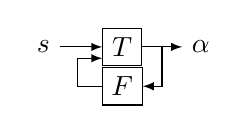
\begin{tikzpicture}[>=latex]
    \node[] (input) {$s$};
    \node[block, right of=input] (f) {$T$};
    \node[right of=f] (output) {$\alpha$};
    \node[block, below of=f, node distance=.5cm] (z) {$F$};
    \draw[->] (input) -- (f);
    \draw[->] (f) -- node (mid) {} (output);
    \draw[->] (mid.center) |-  (z);
    \draw[->] (z.west) -- ++(-.3,0) |- ([yshift=1mm]f.south west);
\end{tikzpicture}
\end{center}

This circuit is a well-defined function on streams:

%\begin{lemma}
%\label{lemma-causal-strict}
%If $F: \stream{B} \to \stream{B}$ is strict and $T: \stream{A} \times \stream{B} \to \stream{B}$ is causal, then for fixed $s$ the operator
%$\lambda\alpha.T(s,F(\alpha)): \stream{A} \to \stream{B}$ is strict.
%\end{lemma}

\begin{lemma}\label{feedback-semantics}
\label{cor-loop}
If $F: \stream{B} \to \stream{B}$ is strict and $T: \stream{A} \times \stream{B} \to \stream{B}$ is causal,
the operator $Q(s)=\fix{\alpha}{T(s,F(\alpha))}$ is well-defined and causal.
If, moreover, $F$ and $T$ are TI then so is $Q$.
\end{lemma}

All \dbsp computations are built using just lifted functions and
delays.  We add two more operators in \secref{sec:nested}.

\subsection{Integration and differentiation}\label{sec:abelianstreams}

Remember that we require the elements of a stream to come from an abelian group $A$.
Streams themselves form an abelian group:

\begin{proposition}
The structure $(\stream{A},+,0,-)$, obtained by lifting the $+$ and unary $-$ operations of $A$,
is an abelian group.  0 is the stream with all values $0_A$.
\end{proposition}

\noindent
Stream addition and negation are causal, TI operators.

\begin{definition}
Given abelian groups $A$ and $B$ we call a stream operator
$S: \stream{A} \rightarrow \stream{B}$ \defined{linear} if it is a group homomorphism, that is,
$S(a+b)=S(a)+S(b)$ (and therefore $S(0)=0$ and $S(-a)=-S(a)$).
\end{definition}

Given a linear function $f: A \to B$, the stream operator $\lift{f}$
is linear and TI (LTI).  $\zm$ is also LTI.

\begin{definition}(bilinear)
A function of two arguments $f: A \times B \to C$ with $A, B, C$ groups, is \emph{bilinear}
if it is linear separately in each argument (i.e., it distributes over addition):
$\forall a, b, c, d . f(a+b, c) = f(a, c) + f(b, c)$, and $f(a, c+d) = f(a, c) + f(c, d).$
\end{definition}

This definition extends to stream operators.
The lifting a bilinear function $f$ is
a bilinear stream operator $\lift{f}$.  An example
is lifted multiplication:
$f: \stream{\N} \times \stream{\N} \to \stream{\N}, f(a, b)[t] = a[t]\cdot b[t]$.

%The composition of (bi)linear operators with linear operators
%is (bi)linear (since homomorphisms compose).

The ``feedback loop'' of a linear operator is linear:

\begin{proposition}
\label{prop-rec-linear}
Let $S$ be a unary, causal, LTI operator. The
operator $Q(s)=\fix{\alpha}{S(s+\zm(\alpha))}$ is well-defined and LTI:

\begin{center}
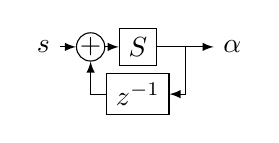
\begin{tikzpicture}[>=latex]
    \node[] (input) {$s$};
    \node[block, shape=circle, right of=input, inner sep=0pt, node distance=.6cm] (plus) {$+$};
    \node[block, right of=plus, node distance=.6cm] (Q) {$S$};
    \node[right of=Q, node distance=1.2cm] (output) {$\alpha$};
    \node[block, below of=Q, node distance=.6cm] (z) {$\zm$};
    \draw[->] (input) -- (plus);
    \draw[->] (plus) -- (Q);
    \draw[->] (Q) -- node (mid) {} (output);
    \draw[->] (mid.center) |-  (z);
    \draw[->] (z) -| (plus);
\end{tikzpicture}
\end{center}
\end{proposition}

\begin{definition}[Differentiation]
The \defined{differentiation operator} $\D_{\stream{A}} : \stream{A} \to \stream{A}$ is defined by:
$\D(s) \defn s - \zm(s)$.

\begin{center}
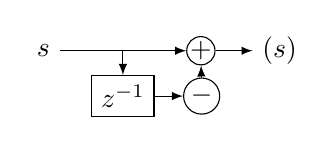
\begin{tikzpicture}[auto,>=latex,node distance=1cm]
    \node[] (input) {$s$};
    \node[block, shape=circle, right of=input, inner sep=0pt,node distance=2cm] (plus) {$+$};
    \node[right of=plus] (output) {$\D(s)$};
    \draw[draw,->] (input) -- node (i) {} (plus);
    \node[block, below of=i, node distance=.7cm] (z) {$\zm$};
    \node[block, shape=circle, right of=z, inner sep=1pt] (minus) {$-$};
    \draw[->] (plus) -- (output);
    \draw[->] (i) -- (z);
    \draw[->] (z) -- (minus);
    \draw[->] (minus) -- (plus);
\end{tikzpicture}
\end{center}
\end{definition}
We generally omit the type, and write just $\D$.
The value of $\D(s)[t] = s[t] - s[t-1]$ if $t > 0$.
\ifstreamexamples
As an example, $\D(\id) = \sv{0 1 1 1 1}$.
\fi

If $s$ is a stream, then $\D(s)$ is the \emph{stream of changes} of $s$.

\begin{proposition}
\label{prop-diff-properties}
$\D$ is causal and LTI.
\end{proposition}

The integration operator ``reconstitutes'' a stream from its changes:

\begin{definition}[Integration]
The \defined{integration operator}  $\I_{\stream{A}} : \stream{A} \to \stream{A}$
is defined by $\I(s) \defn \lambda s . \fix{\alpha}{(s + \zm(\alpha))}$:
\begin{center}
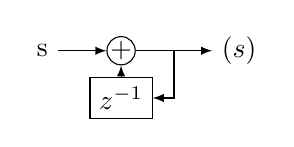
\begin{tikzpicture}[auto,>=latex]
    \node[] (input) {s};
    \node[block, shape=circle, right of=input, inner sep=0pt] (plus) {$+$};
    \node[right of=plus, node distance=1.5cm] (output) {$\I(s)$};
    \node[block, below of=plus, node distance=.6cm] (z) {$z^{-1}$};
    \draw[->] (input) -- (plus);
    \draw[->] (plus) -- node (o) {} (output);
    \draw[->] (o) |- (z);
    \draw[->] (z) -- (plus);
\end{tikzpicture}
\end{center}
\end{definition}

\noindent
We also generally omit the type, and write just $\I$.
This is the construction from Proposition~\ref{prop-rec-linear}
using the identity function for $S$.

\begin{proposition}
$\I(s)$ is the discrete (indefinite) integral applied to the stream $s$:
$\I(s)[t] = \sum_{i \leq t} s[i]$.
\end{proposition}
\ifstreamexamples
As an example, $\I(\id) = \sv{0 1 3 6 10}$.
\fi

\begin{proposition}
\label{prop-integ-properties}
$\I$ is causal and LTI.
\end{proposition}

\begin{theorem}[Inversion]
\label{inverses}
Integration and differentiation are inverses of each other:
$\forall s . \I(\D(s)) = \D(\I(s)) = s$.
\end{theorem}

\noindent
\begin{tabular}{m{2.5cm}m{.3cm}m{1cm}m{.3cm}m{2.5cm}}
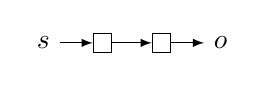
\begin{tikzpicture}[auto,>=latex, node distance=.75cm]
    \node[] (input) {$s$};
    \node[block, right of=input] (I) {$\I$};
    \node[block, right of=I] (D) {$\D$};
    \node[right of=D] (output) {$o$};
    \draw[->] (input) -- (I);
    \draw[->] (I) -- (D);
    \draw[->] (D) -- (output);
\end{tikzpicture}
     &
     $\cong$
     &
     \hspace{-2ex}
\begin{tikzpicture}[auto,>=latex, node distance=.75cm]
    \node[] (input) {$s$};
    \node[right of=input] (output) {$o$};
    \draw[->] (input) -- (output);
\end{tikzpicture}
     &
     $\cong$
     &
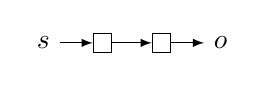
\begin{tikzpicture}[auto,>=latex, node distance=.75cm]
    \node[] (input) {$s$};
    \node[block, right of=input] (D) {$\D$};
    \node[block, right of=D] (I) {$\I$};
    \node[right of=I] (output) {$o$};
    \draw[->] (input) -- (D);
    \draw[->] (D) -- (I);
    \draw[->] (I) -- (output);
\end{tikzpicture}
\end{tabular}

\section{Incremental view maintenance}\label{sec:incremental}

Here we define of IVM and analyze its properties.

\begin{definition}
Given a unary stream operator $Q: \stream{A} \to \stream{B}$ we define the
\defined{incremental version} of $Q$ as:
\begin{equation}\label{def:inc}
\inc{Q} \defn \D \circ Q \circ \I.
\end{equation}
$\inc{Q}$ has the same ``type'' as $Q$: $\inc{Q}: \stream{A} \to \stream{B}$.
For an operator with multiple inputs we define
the incremental version by applying $\I$ to each input independently:
e.g., if $T: \stream{A} \times \stream{B} \rightarrow \stream{C}$ then
$\inc{T}(a, b) \defn \D (T(\I(a), \I(b)))$.
\end{definition}

%The following diagram illustrates the intuition behind this
%definition:
\begin{center}
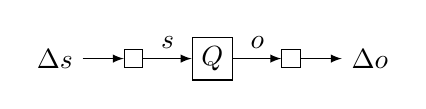
\begin{tikzpicture}[auto,>=latex]
    \node[] (input) {$\Delta s$};
    \node[block, right of=input] (I) {$\I$};
    \node[block, right of=I] (Q) {$Q$};
    \node[block, right of=Q] (D) {$\D$};
    \node[right of=D] (output) {$\Delta o$};
    \draw[->] (input) -- (I);
    \draw[->] (I) -- node (s) {$s$} (Q);
    \draw[->] (Q) -- node (o) {$o$} (D);
    \draw[->] (D) -- (output);
\end{tikzpicture}
\end{center}
If $Q(s) = o$ is a computation, then $\inc{Q}$ performs
the ``same'' computation as $Q$,
but between streams of changes $\Delta s$ and $\Delta o$.

Notice that our definition of incremental computation is meaningful only for \emph{streaming}
computations; this is in contrast to classic definitions, e.g.~\cite{gupta-idb95} which
consider only one change.  Generalizing the definition to operate on streams gives us
additional power, especially when operating with recursive queries.

The following proposition is one of our central results:

\begin{proposition}(Properties of the incremental version):
\label{prop-inc-properties}
\begin{description}[nosep, leftmargin=\parindent]
\item[inversion:] $Q\mapsto\inc{Q}$ is bijective; its inverse is $Q\mapsto \I\circ Q\circ\D$.
\item[invariance:] $\inc{+} = +, \inc{(\zm)} = \zm, \inc{-} = -, \inc{\I}=\I, \inc{\D}=\D$
\item[push/pull:] \label{prop-part-commutation}
    $Q \circ \I = \I \circ \inc{Q}$; $\D\circ Q = \inc{Q}\circ\D$
\item[chain:] $\inc{(Q_1\circ Q_2)} = \inc{Q_1}\circ\inc{Q_2}$ (Generalizes to multiple inputs.)
\item[add:] $\inc{(Q_1 + Q_2)} = \inc{Q_1} + \inc{Q_2}$
\item[cycle:] $\inc{(\lambda s. \fix{\alpha}{T(s,\zm(\alpha)}))} = \lambda s. \fix{\alpha}{\inc{T}(s,\zm(\alpha)})$
\end{description}
\end{proposition}

The \defined{chain rule} states that these two circuits are
equivalent:

\noindent
\begin{tabular}{m{4cm}m{.2cm}m{2.5cm}}
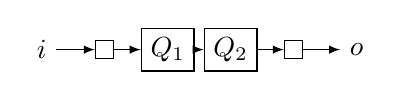
\begin{tikzpicture}[auto,>=latex,node distance=.8cm]
  \node[] (input) {$i$};
  \node[block, right of=input] (I) {$\I$};
  \node[block, right of=I] (Q1) {$Q_1$};
  \node[block, right of=Q1] (Q2) {$Q_2$};
  \node[block, right of=Q2] (D) {$\D$};
  \node[right of=D] (output)  {$o$};
  \draw[->] (input) -- (I);
  \draw[->] (I) -- (Q1);
  \draw[->] (Q1) -- (Q2);
  \draw[->] (Q2) -- (D);
  \draw[->] (D) -- (output);
\end{tikzpicture} &
$\cong$ &
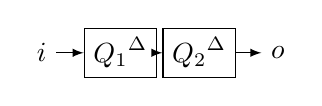
\begin{tikzpicture}[>=latex]
  \node[] (input) {$i$};
  \node[block, right of=input] (Q1) {$\inc{Q_1}$};
  \node[block, right of=Q1] (Q2) {$\inc{Q_2}$};
  \node[right of=Q2] (output)  {$o$};
  \draw[->] (input) -- (Q1);
  \draw[->] (Q1) -- (Q2);
  \draw[->] (Q2) -- (output);
\end{tikzpicture}
\end{tabular}

\noindent In other words, \textbf{to incrementalize a composite query you can incrementalize
each sub-query independently}.  This gives us a simple, syntax-directed, deterministic recipe
for computing the incremental version of an arbitrarily complex query.

The \defined{cycle rule} states that the following circuits are equivalent:

\noindent
\begin{tabular}{m{4.2cm}m{.2cm}m{3cm}}
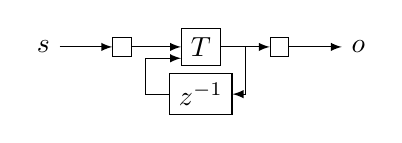
\begin{tikzpicture}[>=latex]
    \node[] (input) {$s$};
    \node[block, right of=input] (I) {$\I$};
    \node[block, right of=I] (f) {$T$};
    \node[block, right of=f] (D) {$\D$};
    \node[right of=D] (output) {$o$};
    \node[block, below of=f, node distance=.6cm] (z) {$\zm$};
    \draw[->] (input) -- (I);
    \draw[->] (I) -- (f);
    \draw[->] (f) -- node (mid) {} (D);
    \draw[->] (mid.center) |-  (z);
    \draw[->] (z.west) -- ++(-.3,0) |- ([yshift=1mm]f.south west);
    \draw[->] (D) -- (output);
\end{tikzpicture} & $\cong$ &
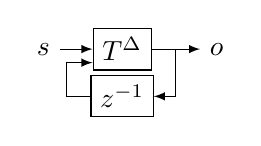
\begin{tikzpicture}[>=latex]
    \node[] (input) {$s$};
    \node[block, right of=input] (f) {$\inc{T}$};
    \node[right of=f, node distance=1.2cm] (output) {$o$};
    \node[block, below of=f, node distance=.6cm] (z) {$\zm$};
    \draw[->] (input) -- (f);
    \draw[->] (f) -- node (mid) {} (output);
    \draw[->] (mid.center) |-  (z);
    \draw[->] (z.west) -- ++(-.3,0) |- ([yshift=1mm]f.south west);
\end{tikzpicture}
\end{tabular}

In other words, the incremental version of a feedback loop around a query
is just the feedback loop with the incremental query for its body.  The significance
of this result will be apparent when we implement recursive queries.

To execute incremental queries efficiently, we want to compute directly
on streams of changes, without integrating them. The invariance property above shows
that stream operators $+$, $-$, and $\zm$ are identical to their incremental versions.
The following theorems generalize this to linear and bi-linear operators:

\begin{theorem}[Linear]\label{linear}
For an LTI operator $Q$ we have $\inc{Q}=Q$.
\end{theorem}

\begin{theorem}[Bilinear]\label{bilinear}
For a bilinear TI operator $\times$ we have
$\inc{(a \times b)} ~=~ a \times b ~+~ \zm(\I(a)) \times b ~+~ a \times \zm(\I(b))
= \I(a) \times b + a \times \zm(\I(b))$.
In pictures: \\
\noindent
\begin{tabular}{m{2.2cm}m{0cm}m{2.3cm}m{0cm}m{2.8cm}}
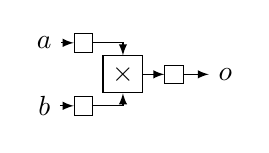
\begin{tikzpicture}[auto,node distance=.65cm,>=latex]
    \node[] (a) {$a$};
    \node[block, right of=a, node distance=.5cm] (ai) {$\I$};
    \node[below of=a, node distance=.4cm] (midway) {};
    \node[below of=midway, node distance=.4cm] (b) {$b$};
    \node[block, right of=b, node distance=.5cm] (bi) {$\I$};
    \node[block, right of=midway, node distance=1cm] (q) {$\times$};
    \node[block, right of=q] (D) {$\D$};
    \node[right of=D] (output) {$o$};
    \draw[->] (a) -- (ai);
    \draw[->] (b) -- (bi);
    \draw[->] (ai) -| (q);
    \draw[->] (bi) -| (q);
    \draw[->] (q) -- (D);
    \draw[->] (D) -- (output);
\end{tikzpicture} &
$\cong$ &
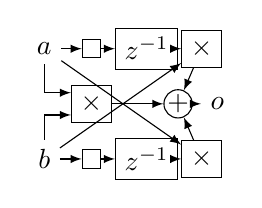
\begin{tikzpicture}[auto,>=latex,node distance=.7cm]
  \node[] (input1) {$a$};
  \node[below of=input1, node distance=1.4cm] (input2) {$b$};
  \node[block, right of=input1, node distance=.6cm] (I1) {$\I$};
  \node[block, below of=I1] (ab) {$\times$};
  \node[block, right of=input2, node distance=.6cm] (I2) {$\I$};
  \draw[->] (input1) -- (I1);
  \draw[->] (input2) -- (I2);
  \draw[->] (input1) |- ([yshift=-1mm]ab.north west);
  \draw[->] (input2) |- ([yshift=1mm]ab.south west);
  \node[block, right of=I1] (ZI1) {$\zm$};
  \node[block, right of=I2] (ZI2) {$\zm$};
  \draw[->] (I1) -- (ZI1);
  \draw[->] (I2) -- (ZI2);
  \node[block, right of=ZI1] (DI1) {$\times$};
  \node[block, right of=ZI2] (DI2) {$\times$};
  \draw[->] (ZI1) -- (DI1);
  \draw[->] (ZI2) -- (DI2);
  \node[block, circle, right of=ab, inner sep=0cm, node distance=1.1cm] (sum) {$+$};
  \draw[->] (ab) -- (sum);
  \draw[->] (DI1) -- (sum);
  \draw[->] (DI2) -- (sum);
  \node[right of=sum, node distance=.5cm] (output) {$o$};
  \draw[->] (sum) -- (output);
  \draw[->] (input1) -- (DI2);
  \draw[->] (input2) -- (DI1);
\end{tikzpicture}
&
$\cong$ &
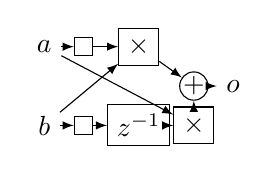
\begin{tikzpicture}[auto,>=latex,node distance=.7cm]
  \node[] (input1) {$a$};
  \node[below of=input1, node distance=1cm] (input2) {$b$};
  \node[block, right of=input1, node distance=.5cm] (I1) {$\I$};
  \node[block, right of=input2, node distance=.5cm] (I2) {$\I$};
  \draw[->] (input1) -- (I1);
  \draw[->] (input2) -- (I2);
  \node[block, right of=I2] (ZI2) {$\zm$};
  \draw[->] (I2) -- (ZI2);
  \node[block, right of=I1] (DI1) {$\times$};
  \node[block, right of=ZI2] (DI2) {$\times$};
  \draw[->] (I1) -- (DI1);
  \draw[->] (ZI2) -- (DI2);
  \node[block, circle, above of=DI2, inner sep=0cm, node distance=.5cm] (sum) {$+$};
  \draw[->] (DI1) -- (sum);
  \draw[->] (DI2) -- (sum);
  \node[right of=sum, node distance=.5cm] (output) {$o$};
  \draw[->] (sum) -- (output);
  \draw[->] (input1) -- (DI2);
  \draw[->] (input2) -- (DI1);
\end{tikzpicture}
\end{tabular}
\end{theorem}

Rewriting Theorem~\ref{bilinear} using $\Delta a$ for the stream of changes to $a$ we
get the familiar formula for incremental equi-joins:
$\Delta(a\times b) =\Delta a \times \Delta b + a\times(\Delta b) +
(\Delta a)\times b$; equi-joins are indeed bilinear.


\part{Incremental view maintenance in \dbsp}

\section{Relational algebra in \dbsp}\label{sec:relational}

Results in \secref{sec:streams} apply to streams of arbitrary group
values.  In this section we turn our attention to using these results
in the context of relational databases.

However, we face a technical problem: the $\I$ and $\D$ operators were
defined on abelian groups, and relational databases in general are
not abelian groups, since they operate on sets.  Fortunately,
there is a well-known tool in the database literature
which converts set operations into group operations by using \zrs
(also called z-relations~\cite{green-pods07}) instead of sets.

We start by defining the \zrs group, and then we explain how
relational queries are converted into \dbsp circuits over \zrs.

\subsection{\zrs as an abelian group}

Given a set $A$ we define \defined{\zrs}\footnote{Also called $\Z$-relations elsewhere~\cite{green-tcs11}.}
over $A$ as functions with \emph{finite support} from $A$ to $\Z$ (i.e., which are 0 almost everywhere).
These are functions $f: A \rightarrow \Z$ where
$f(x) \not= 0$ for at most a finite number of values $x \in A$.
We also write $\Z[A]$ for the type of \zrs with elements from $A$.
The values in $\Z[A]$ can also be thought as being key-value maps with
keys in $A$ and values in $\Z$, justifying the array indexing notation.

Since $\Z$ is an abelian group, $\Z[A]$ is also an abelian group.  This group
$(\Z[A], +_{\Z[A]}, 0_{\Z[A]}, -_{\Z{A}})$ has addition and subtraction defined pointwise:
$$(f +_{\Z[A]} g)(x) = f(x) + g(x) . \forall x \in A.$$
The $0$ element of $\Z[A]$ is the function $0_{\Z[A]}$ defined by $0_{\Z[A]}(x) = 0 . \forall x \in A$.
(In fact, since $\Z$ is a ring, $\Z[A]$ is also ring, endowed with a multiplication operation,
also defined pointwise.)

A particular \zr $m \in \Z[A]$ can be denoted by enumerating the inputs that map to non-zero values and
their multiplicities:
$m = \{ x_1 \mapsto w_1, \dots, x_n \mapsto w_n \}$.
We call $w_i \in Z$ the \defined{multiplicity} (or weight)
of $x_i \in A$.  Multiplicities can be negative.
We write that $x \in m$ for $x \in A$, iff $m[x] \not= 0$.

For example, let's consider a concrete \zr $R \in \Z[\texttt{string}]$,
defined by $R = \{ \texttt{joe} \mapsto 1, \texttt{anne} \mapsto -1 \}$.
$R$ has two elements in its domain,
\texttt{joe} with a multiplicity of 1 (so $R[\texttt{joe}] = 1$),
and \texttt{anne} with a multiplicity of $-1$.
We say \texttt{joe} $\in R$ and \texttt{anne} $\in R$.

Given a \zr $m \in \Z[A]$ and a value $v \in A$, we overload the array index notation
$m[v]$ to denote the multiplicity of the element $v$ in $m$.
Thus we write $R[\texttt{anne}] = -1$.
When $c \in \Z$, and $v \in A$ we also write $c \cdot v$ for the \defined{singleton} \zr $\{
v \mapsto c \}$.  In other words, $3 \cdot \texttt{frank} = \{ \texttt{frank} \mapsto 3 \}$.
We extend scalar multiplication to operate on \zrs: for $c \in Z, m \in \Z[A]$,
$c \cdot m \defn \sum_{x \in m} (c \cdot m[x]) \cdot x$.  We then have
$2 \cdot R = \{ \texttt{joe} \mapsto 2, \texttt{anne} \mapsto -2 \}$: multiplying
each row weight by 2.

We define the \defined{size} of a \zr as the size of its support set, and we use the
modulus symbol to represent the size: $|m| \defn \sum_{x \in m} 1$.  So $|R| = 2$.

\subsection{Sets, bags, and \zrs}

\zrs generalize sets and bags.
Given a set with elements from $A$, it can be represented as a \zr $\Z[A]$
by associating a weight of 1 with each set element.  The function $\mbox{tozset}: 2^A \to \Z[A]$,
defined as $\mbox{tozset}(s) = \sum_{x \in s} 1 \cdot x$,
converts a set to a \zr by associating a multiplicity of 1 with each set element.
Thus $\mbox{tozset}(\{ \code{joe}, \code{anne} \}) = \{ \code{joe} \mapsto 1, \code{anne} \mapsto 1 \}$.

\begin{definition}
We say that a \zr represents a \defined{set} if the multiplicity of every
element is one.  We define a function to check this property
$\isset : \Z[A] \rightarrow \B$\index{isset}, given by:
$$\isset(m) \defn \left\{
\begin{array}{ll}
  \mbox{true} & \mbox{ if } m[x] = 1, \forall x \in m \\
  \mbox{false} & \mbox{ otherwise}
\end{array}
\right.
$$
\end{definition}
For our example $\isset(R) = \mbox{false}$, since $R[\texttt{anne}] = -1$.
$\isset(\mbox{tozset}(m)) = \mbox{true}$ for any set $m \in 2^A$.

\begin{definition}
We say that a \zr is \defined{positive} (or a \defined{bag}) if the multiplicity of every element is
positive. We define a function to check this property
$\ispositive : \Z[A] \rightarrow \B$\index{ispositive}, given by
$$\ispositive(m) \defn \left\{
\begin{array}{ll}
  \mbox{true} & \mbox{ if } m[x] \geq 0, \forall x \in A \\
  \mbox{false} & \mbox{ otherwise}
\end{array}
\right.$$
\end{definition}
For our example $\ispositive(R) = \mbox{false}$, since $R[\texttt{anne}] = -1$,
but $\isset(m) \Rightarrow \ispositive(m). \forall m \in \Z[A]$.

We also write $m \geq 0$ when $m$ is
positive.  For positive $m, n$ we write $m \geq n$ for $m, n
\in \Z[A]$ iff $m - n \geq 0$.  The relation $\geq$ is a partial order.

\begin{definition}
The function $\distinct: \Z[A] \rightarrow \Z[A]$\index{distinct}
projects a \zr into an underlying set (but \emph{the result is
  still a \zr}).  The definition is $\forall x \in A$
$$\distinct(m)[x] \defn \left\{
\begin{array}{ll}
  1 & \mbox{ if } m[x] > 0 \\
  0 & \mbox{ otherwise}
\end{array}
\right.
$$
\end{definition}
$\distinct(R) = \{ \texttt{joe} \mapsto 1 \}$.

$\distinct$ ``removes'' elements with negative multiplicities.  $\zpp{\distinct}$.

Circuits derived from relational program will only operate with positive \zrs;
non-positive values will be only used to represent \emph{changes} to \zrs
(a change with negative weights will remove elements from a \zr).

\begin{proposition}
$\distinct$ is idempotent: $\distinct = \distinct \circ \distinct$.
\end{proposition}

\begin{proposition}
For any $m \in \Z[A]$ we have: $\isset(\distinct(m))$ and \\
$\ispositive(\distinct(m))$.
\end{proposition}

We call a function $f : \Z[I] \rightarrow \Z[O]$ \defined{positive} if
$\forall x \in \Z[I], x \geq 0_{\Z[I]} \Rightarrow f(x) \geq 0_{\Z[0]}$.
We extend the notation used for \zrs for functions as well: $\ispositive(f)$.

\paragraph{Correctness of the \dbsp implementations}

The function $\mbox{toset}: \Z[A] \to 2^A$, defined as $\mbox{toset}(m) =
\cup_{x \in \distinct(m)} \{ x \}$, converts a \zr into a set.

A relational query $f$ that transforms
a set $V$ into a set $U$ will be implemented by a \dbsp computation $f'$ on
\zrs.  The correctness of the implementation requires that the following
diagram commutes:

\begin{center}
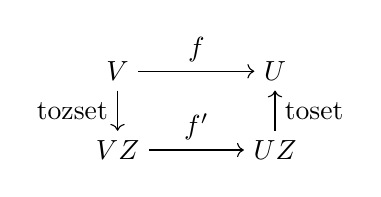
\begin{tikzpicture}
  \node[] (V) {$V$};
  \node[below of=V] (VZ) {$VZ$};
  \node[right of=V, node distance=2cm] (U) {$U$};
  \node[below of=U] (UZ) {$UZ$};
  \draw[->] (V) -- node (f) [above] {$f$} (U);
  \draw[->] (V) --  node (s) [left] {tozset}(VZ);
  \draw[->] (VZ) -- node (f) [above] {$f'$} (UZ);
  \draw[->] (UZ) -- node (d) [right] {toset} (U);
\end{tikzpicture}
\end{center}

\textbf{Remark:} We can generalize the notion of \zrs to functions $m: A \to \mathbf{G}$ for a
ring $\mathbf{G}$ other than $\Z$.  The properties we need from the ring structure are the
following: the ring must be a commutative group (needed for defining $\I$, $\D$, and $\zm$),
the multiplication operation must distribute over addition (needed to define
Cartesian products), and there must be a notion of positive values, needed
to define the $\distinct$ function.  Rings such as $\mathbb{Q}$ or $\mathbb{R}$
would work perfectly.

\subsection{Streams over \zrs}

Since all the results from Section~\ref{sec:streams} are true for streams
over an arbitrary abelian group, they extend to streams where the elements
are \zrs.  In the rest of this text we only consider streams of the form $\stream{\Z[A]}$, for
some element type $A$.

An example of a stream of \zrs is \\ $s = \sv{0 R -1\cdot{R} 2\cdot{R} -2\cdot{R}}$.
We have $s[2] = -R = \{ \texttt{joe} \mapsto -1, \texttt{anne} \mapsto 1 \}$.

\begin{definition}
A stream $s \in \stream{\Z[A]}$ is \defined{positive} if every value of the stream is positive:
$s[t] \geq 0 . \forall t \in \N$.
\end{definition}



\begin{definition}
A stream $s \in \stream{\Z[A]}$ is \defined{monotone} if $s[t] \geq s[t-1], \forall t \in \N$.
\end{definition}

\begin{lemma}
Given a positive stream $s \in \stream{\Z[A]}$ the stream $\I(s)$ is monotone.
\end{lemma}
\begin{proof}
  Let us compute $\I(s)[t + 1] - \I(s)[t] = \sum_{i \leq t+1}s[i] -
  \sum_{i \leq t}s[i] = s[t+1] \geq 0$, by commutativity and positivity of $s$.
\end{proof}

\begin{lemma}
Given a monotone stream $s \in \stream{\Z[A]}$, the
elements of the stream $\D(s)$ are positive.
\end{lemma}
\begin{proof}
  By the definition of monotonicity $s[t+1] \geq s[t]$.  By definition
  of $\D$ we have $\D(s)[t+1] = s[t+1] - s[t] \geq 0$.
\end{proof}

\subsection{Implementing the relational algebra}\label{sec:relational-operators}

The fact that the relational algebra can be implemented by computations
on \zrs has been shown before, e.g.~\cite{green-pods07}.  The translation
of the core relational operators is summarized in Table~\ref{tab:relational} and discussed below.

\begin{table*}
\begin{center}
\footnotesize
\begin{tabular}{|m{1.2cm}m{4.2cm}m{5cm}|} \hline
Operation & SQL example & \dbsp circuit  \\ \hline
Composition &
 \begin{lstlisting}[language=SQL]
SELECT DISTINCT ... FROM
(SELECT ... FROM ...)
\end{lstlisting}
 &
 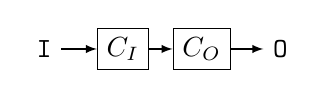
\begin{tikzpicture}[auto,>=latex]
  \node[] (I) {\code{I}};
  \node[block, right of=I] (CI) {$C_I$};
  \draw[->] (I) -- (CI);
  \node[block, right of=CI] (CO) {$C_O$};
  \node[right of=CO] (O) {\code{O}};
  \draw[->] (CI) -- (CO);
  \draw[->] (CO) -- (O);
\end{tikzpicture}
\\ \hline
Union &
\begin{lstlisting}[language=SQL]
(SELECT * FROM I1)
UNION
(SELECT * FROM I2)
\end{lstlisting}
&
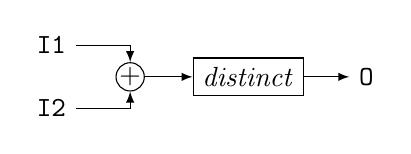
\begin{tikzpicture}[auto,>=latex]
  \node[] (input1) {\code{I1}};
  \node[below of=input1, node distance=.4cm] (midway) {};
  \node[below of=midway, node distance=.4cm] (input2) {\code{I2}};
  \node[block, shape=circle, right of=midway, inner sep=0in] (plus) {$+$};
  \node[block, right of=plus, node distance=1.5cm] (distinct) {$\distinct$};
  \node[right of=distinct, node distance=1.5cm] (output) {\code{O}};
  \draw[->] (input1) -| (plus);
  \draw[->] (input2) -| (plus);
  \draw[->] (plus) -- (distinct);
  \draw[->] (distinct) -- (output);
\end{tikzpicture}
\\ \hline
Projection &
\begin{lstlisting}[language=SQL]
SELECT DISTINCT I.c
FROM I
\end{lstlisting}
&
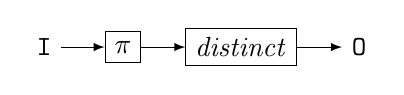
\begin{tikzpicture}[auto,>=latex]
  \node[] (input) {\code{I}};
  \node[block, right of=input] (pi) {$\pi$};
  \node[block, right of=pi, node distance=1.5cm] (distinct) {$\distinct$};
  \node[right of=distinct, node distance=1.5cm] (output) {\code{O}};
  \draw[->] (input) -- (pi);
  \draw[->] (pi) -- (distinct);
  \draw[->] (distinct) -- (output);
\end{tikzpicture}
\\ \hline
Filtering &
\begin{lstlisting}[language=SQL]
SELECT * FROM I
WHERE p(I.c)
\end{lstlisting}
&
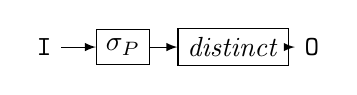
\begin{tikzpicture}[auto,>=latex]
  \node[] (input) {\code{I}};
  \node[block, right of=input] (map) {$\sigma_P$};
  \node[block, right of=map, node distance=1.4cm] (distinct) {$\distinct$};
  \node[right of=distinct] (output) {\code{O}};
  \draw[->] (input) -- (map);
  \draw[->] (map) -- (distinct);
  \draw[->] (distinct) -- (output);
\end{tikzpicture}
\\ \hline
Selection &
\begin{lstlisting}[language=SQL]
SELECT DISTINCT f(I.c, ...)
FROM I
\end{lstlisting}
&
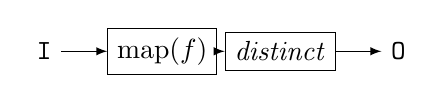
\begin{tikzpicture}[auto,>=latex]
  \node[] (input) {\code{I}};
  \node[block, right of=input, node distance=1.5cm] (map) {$\mbox{map}(f)$};
  \node[block, right of=map, node distance=1.5cm] (distinct) {$\distinct$};
  \node[right of=distinct, node distance=1.5cm] (output) {\code{O}};
  \draw[->] (input) -- (map);
  \draw[->] (map) -- (distinct);
  \draw[->] (distinct) -- (output);
\end{tikzpicture}
\\ \hline
\parbox[b][][t]{1cm}{
Cartesian \\
product} &
\begin{lstlisting}[language=SQL]
SELECT I1.*, I2.*
FROM I1, I2
\end{lstlisting}
&
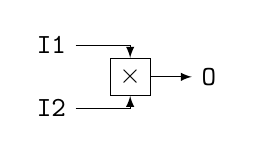
\begin{tikzpicture}[auto,>=latex]
  \node[] (i1) {\code{I1}};
  \node[below of=i1, node distance=.4cm] (midway) {};
  \node[below of=midway, node distance=.4cm] (i2) {\code{I2}};
  \node[block, right of=midway] (prod) {$\times$};
  \node[right of=prod] (output) {\code{O}};
  \draw[->] (i1) -| (prod);
  \draw[->] (i2) -| (prod);
  \draw[->] (prod) -- (output);
\end{tikzpicture}
\\ \hline
Join &
\begin{lstlisting}[language=SQL]
SELECT I1.*, I2.*
FROM I1 JOIN I2
ON I1.c1 = I2.c2
\end{lstlisting}
&
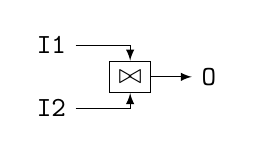
\begin{tikzpicture}[auto,>=latex]
  \node[] (i1) {\code{I1}};
  \node[below of=i1, node distance=.4cm] (midway) {};
  \node[below of=midway, node distance=.4cm] (i2) {\code{I2}};
  \node[block, right of=midway] (prod) {$\bowtie$};
  \node[right of=prod] (output) {\code{O}};
  \draw[->] (i1) -| (prod);
  \draw[->] (i2) -| (prod);
  \draw[->] (prod) -- (output);
\end{tikzpicture}
\\ \hline
Intersection &
\begin{lstlisting}[language=SQL]
(SELECT * FROM I1)
INTERSECT
(SELECT * FROM I2)
\end{lstlisting}
&
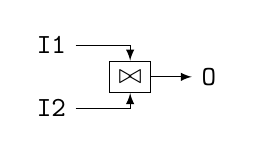
\begin{tikzpicture}[auto,>=latex]
  \node[] (i1) {\code{I1}};
  \node[below of=i1, node distance=.4cm] (midway) {};
  \node[below of=midway, node distance=.4cm] (i2) {\code{I2}};
  \node[block, right of=midway] (prod) {$\bowtie$};
  \node[right of=prod] (output) {\code{O}};
  \draw[->] (i1) -| (prod);
  \draw[->] (i2) -| (prod);
  \draw[->] (prod) -- (output);
\end{tikzpicture}
\\ \hline
Difference &
\begin{lstlisting}[language=SQL]
SELECT * FROM I1
EXCEPT
SELECT * FROM I2
\end{lstlisting}
&
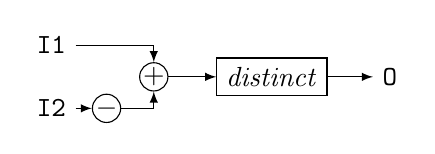
\begin{tikzpicture}[auto,>=latex, node distance=.7cm]
  \node[] (i1) {\code{I1}};
  \node[below of=i1, node distance=.4cm] (midway) {};
  \node[below of=midway, node distance=.4cm] (i2) {\code{I2}};
  \node[block, shape=circle, inner sep=0in, right of=i2] (m) {$-$};
  \node[block, right of=midway, shape=circle, inner sep=0in, node distance=1.3cm] (plus) {$+$};
  \node[block, right of=plus, node distance=1.5cm] (distinct) {$\distinct$};
  \node[right of=distinct, node distance=1.5cm] (output) {\code{O}};
  \draw[->] (i1) -| (plus);
  \draw[->] (i2) -- (m);
  \draw[->] (m) -| (plus);
  \draw[->] (plus) -- (distinct);
  \draw[->] (distinct) -- (output);
\end{tikzpicture}
\\ \hline
\end{tabular}
\caption{Implementation of SQL relational set operators in \dbsp.
Each query assumes that inputs \code{I}, \code{I1}, \code{I2}, are sets and it
produces output sets.\label{tab:relational}}
\end{center}
\end{table*}

The translation is fairly straightforward, but many operators require
the application of a $\distinct$ to produce sets.  The correctness of
this implementation is predicated on the global circuit inputs being
sets as well.

\subsubsection{Query composition}

A composite query is translated by compiling each sub-query separately into a circuit
and composing the respective circuits.

For example, consider the following SQL query:

\begin{lstlisting}[language=SQL]
SELECT ... FROM (SELECT ... FROM ...)
\end{lstlisting}

\noindent given circuits $C_O$ implementing the outer query and $C_I$
implementing the inner query, the translation of the composite query is:

\begin{center}
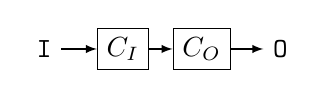
\begin{tikzpicture}[auto,>=latex]
  \node[] (I) {\code{I}};
  \node[block, right of=I] (CI) {$C_I$};
  \draw[->] (I) -- (CI);
  \node[block, right of=CI] (CO) {$C_O$};
  \node[right of=CO] (O) {\code{O}};
  \draw[->] (CI) -- (CO);
  \draw[->] (CO) -- (O);
\end{tikzpicture}
\end{center}

We have $\ispositive(C_I) \land \ispositive(C_0) \Rightarrow \ispositive(C_O \circ C_I)$
and $\zpp{C_I} \land \zpp{C_O} \Rightarrow \zpp{C_O \circ C_I}$.

\subsubsection{Set union}

Consider the following SQL query:

\begin{lstlisting}[language=SQL]
(SELECT * FROM I1) UNION (SELECT * FROM I2)
\end{lstlisting}

The following circuit implements the union program:

\begin{center}
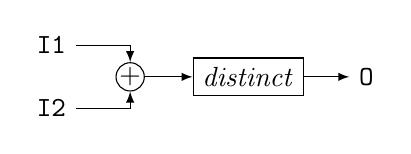
\begin{tikzpicture}[auto,>=latex]
  \node[] (input1) {\code{I1}};
  \node[below of=input1, node distance=.4cm] (midway) {};
  \node[below of=midway, node distance=.4cm] (input2) {\code{I2}};
  \node[block, shape=circle, right of=midway, inner sep=0in] (plus) {$+$};
  \node[block, right of=plus, node distance=1.5cm] (distinct) {$\distinct$};
  \node[right of=distinct, node distance=1.5cm] (output) {\code{O}};
  \draw[->] (input1) -| (plus);
  \draw[->] (input2) -| (plus);
  \draw[->] (plus) -- (distinct);
  \draw[->] (distinct) -- (output);
\end{tikzpicture}
\end{center}

Given \zrs $a, b \in \Z[I]$ s.t. $\isset(a)$ and $\isset(b)$, their \emph{set union}
can be computed as: $\cup: \Z[I] \times \Z[I] \rightarrow \Z[I]$,  $$a
\cup b \defn \distinct(a +_{\Z[I]} b).$$
The $\distinct$ application is necessary to provide the set semantics.

\subsubsection{Projection}
Consider a query such as:

\begin{lstlisting}[language=SQL]
SELECT I.c FROM I
\end{lstlisting}

We can assume without loss of generality that table \code{I} has two columns, and that
a single column is preserved in the projection.
Hence the type of \code{I} is $\Z[A_0 \times A_1]$ while the result has type is $\Z[A_0]$.
In terms of \zrs, the projection of a \zr $i$ on $A_0$ is defined as: $$\pi(i)[y] =
\sum_{x \in i, x|_0 = y} i[x]$$
\noindent where $x|_0$ is first component of the tuple $x$.
In other words, the multiplicity of a tuple in the result is the sum
of the multiplicities of all input tuples that project to it.

The circuit for a projection query is:

\begin{center}
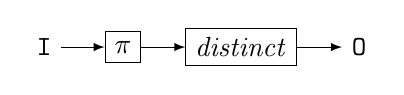
\begin{tikzpicture}[auto,>=latex]
  \node[] (input) {\code{I}};
  \node[block, right of=input] (pi) {$\pi$};
  \node[block, right of=pi, node distance=1.5cm] (distinct) {$\distinct$};
  \node[right of=distinct, node distance=1.5cm] (output) {\code{O}};
  \draw[->] (input) -- (pi);
  \draw[->] (pi) -- (distinct);
  \draw[->] (distinct) -- (output);
\end{tikzpicture}
\end{center}

The $\distinct$ is necessary to convert the result to a set.\\
$\pi$ is linear; $\ispositive(\pi), \zpp{\pi}$.

\subsubsection{Selection}

We generalize the SQL selection operator to allow it to apply an arbitrary function to each row of the
selected set.
Given a function $f : A \rightarrow B$, the mathematical \defined{map} operator ``lifts'' the
function $f$ to operate on \zrs: $\map(f) : \Z[A] \rightarrow \Z[B]$.  A map operator
appears in SQL due to the use of expressions in the SELECT clause, as in the following example:

\begin{lstlisting}[language=SQL]
SELECT f(I.c) FROM I
\end{lstlisting}

The circuit implementation of this query is:

\begin{center}
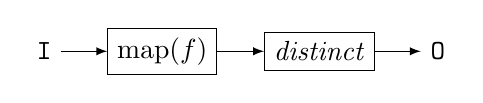
\begin{tikzpicture}[auto,>=latex]
  \node[] (input) {\code{I}};
  \node[block, right of=input, node distance=1.5cm] (map) {$\mbox{map}(f)$};
  \node[block, right of=map, node distance=2cm] (distinct) {$\distinct$};
  \node[right of=distinct, node distance=1.5cm] (output) {\code{O}};
  \draw[->] (input) -- (map);
  \draw[->] (map) -- (distinct);
  \draw[->] (distinct) -- (output);
\end{tikzpicture}
\end{center}

For any function $f$ we have the following properties:
$\map(f)$ is linear, $\ispositive(\map(f)), and \zpp{\map(f)}.$

\subsubsection{Filtering}

Filtering occurs in SQL through a WHERE clause, as in the following example:

\noindent
\begin{lstlisting}[language=SQL]
SELECT * FROM I WHERE p(I.c)
\end{lstlisting}

Let us assume that we are filtering with a predicate
$P: A \rightarrow \B$.  We define the following function $\sigma_P: \Z[A] \rightarrow \Z[A]$ as:
$$\sigma_P(m)[t] = \left\{
\begin{array}{ll}
  m[t] \cdot t & \mbox{ if } P(t) \\
  0 & \mbox{ otherwise } \\
\end{array}
\right.
$$

The circuit for filtering with a predicate $P$ is:

\begin{center}
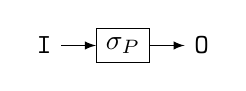
\begin{tikzpicture}[auto,>=latex]
  \node[] (input) {\code{I}};
  \node[block, right of=input] (map) {$\sigma_P$};
  \node[right of=map] (output) {\code{O}};
  \draw[->] (input) -- (map);
  \draw[->] (map) -- (output);
\end{tikzpicture}
\end{center}

For any predicate $P$ we have $\isset(i) \Rightarrow
\isset(\sigma_P(i))$ and $\ispositive(\sigma_P)$.  Thus a $\distinct$
is not needed.  $\sigma_P$ is linear and $\zpp{\sigma_P}$.

\subsubsection{Cartesian products}

Consider this SQL query performing a Cartesian product
between sets \code{I1} and \code{I2}:

\begin{lstlisting}[language=SQL]
SELECT I1.*, I2.* FROM I1, I2
\end{lstlisting}

We first define a product operation on \zrs.
For $a \in \Z[A]$ and $b \in \Z[B]$ we define $a \times b \in \Z[A \times B]$ by
$$(a \times b)((x,y)) \defn a[x] \times b[y] . \forall x \in a, y \in b.$$
The weight of a pair in the result is the product of the weights of the
elements in the sources.  The circuit for the query is:

\begin{center}
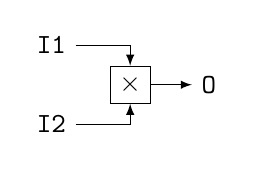
\begin{tikzpicture}[auto,>=latex]
  \node[] (i1) {\code{I1}};
  \node[below of=i1, node distance=.5cm] (midway) {};
  \node[below of=midway, node distance=.5cm] (i2) {\code{I2}};
  \node[block, right of=midway] (prod) {$\times$};
  \node[right of=prod] (output) {\code{O}};
  \draw[->] (i1) -| (prod);
  \draw[->] (i2) -| (prod);
  \draw[->] (prod) -- (output);
\end{tikzpicture}
\end{center}

$\isset(x) \land \isset(y) \Rightarrow \isset(x \times y).$
$\times$ is bilinear, $\ispositive(\times), \zpp{\times}$.

\subsubsection{Joins}

As is well-known, joins can be modeled as Cartesian products
followed by filtering.  Since a join is a composition of a bilinear
and a linear operator, it is also a bilinear operator.
$\ispositive(\bowtie), \zpp{\bowtie}.$

In practice joins are very important computationally, and they are
implemented by a built-in scalar function on \zrs:

$$(a \bowtie b)((x,y)) \defn a[x] \times b[y] \mbox{ if } x|_{c1} = y|_{c2}.$$

\begin{center}
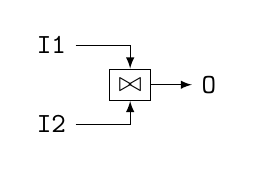
\begin{tikzpicture}[auto,>=latex]
  \node[] (i1) {\code{I1}};
  \node[below of=i1, node distance=.5cm] (midway) {};
  \node[below of=midway, node distance=.5cm] (i2) {\code{I2}};
  \node[block, right of=midway] (prod) {$\bowtie$};
  \node[right of=prod] (output) {\code{O}};
  \draw[->] (i1) -| (prod);
  \draw[->] (i2) -| (prod);
  \draw[->] (prod) -- (output);
\end{tikzpicture}
\end{center}

\subsubsection{Set intersection}

Set intersection is a special case of join, where both relations have the same schema.
It follows that set intersection is bilinear,
and has the zero-preservation property.

\subsubsection{Set difference}  Consider the following query:

\begin{lstlisting}[language=SQL]
SELECT * FROM I1 EXCEPT SELECT * FROM I2
\end{lstlisting}

We define the set difference on \zrs as follows:
$\setminus: \Z[I] \times \Z[I] \rightarrow \Z[I]$, where $$i_1
\setminus i_2 = \distinct(i_1 - i_2).$$  Note
that we have $\forall i_1, i_2, \ispositive(i_1 \setminus
i_2)$ due to the $\distinct$ operator.
The circuit computing the above query is:

\begin{center}
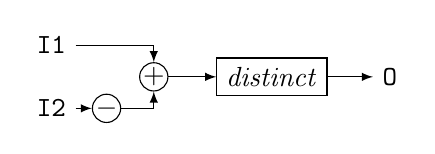
\begin{tikzpicture}[auto,>=latex, node distance=.7cm]
  \node[] (i1) {\code{I1}};
  \node[below of=i1, node distance=.4cm] (midway) {};
  \node[below of=midway, node distance=.4cm] (i2) {\code{I2}};
  \node[block, shape=circle, inner sep=0in, right of=i2] (m) {$-$};
  \node[block, right of=midway, shape=circle, inner sep=0in, node distance=1.3cm] (plus) {$+$};
  \node[block, right of=plus, node distance=1.5cm] (distinct) {$\distinct$};
  \node[right of=distinct, node distance=1.5cm] (output) {\code{O}};
  \draw[->] (i1) -| (plus);
  \draw[->] (i2) -- (m);
  \draw[->] (m) -| (plus);
  \draw[->] (plus) -- (distinct);
  \draw[->] (distinct) -- (output);
\end{tikzpicture}
\end{center}

\section{Recursive queries in \dbsp}\label{sec:recursive}

Recursive queries are very useful in a many applications.
For example, many graph algorithms (such as graph reachability
or transitive closure) are naturally expressed using recursive queries.

We illustrate the implementation of recursive queries in \dbsp for
stratified Datalog.

\subsection{Implementing recursive queries}

For warm-up we start with a single recursive queries, and then we discuss
the case of mutually recursive queries.

\subsubsection{Recursive rules}\label{sec:recursion}

In Datalog a recursive rule appears when a relation that appears in the head of a rule
is also used in a positive term in the rule's body.  (Stratification disallows
the use of the same relation negated in the rule's body).
The Datalog semantics of recursive rules is to compute a fixedpoint.

Consider a Datalog program of the form:

\begin{lstlisting}[language=ddlog]
O(v) :- C(v).  // base case
O(v) :- ..., O(x), I(z), ... .  // recursive case
\end{lstlisting}

Note that relation \code{O} is recursively defined.  Let us assume wlog that the \code{O}
relation depends on two other relations (i.e., in the rule bodies defining \code{O} the
two other relations appear) : a ``base case'' relation \code{C} (which appears in a
non-recursive rule), and a relation \code{I} which appears in the recursive rule, but
does not itself depend on \code{O}.

To implement the computation of \code{O} as a circuit we perform the following algorithm:

\begin{algorithm}[recursive queries]\label{algorithm-rec}
\noindent
\begin{enumerate}[nosep, leftmargin=\parindent]
\item Implement the non-recursive relational query $R$ as described in
    \secref{sec:relational} and Table~\ref{tab:relational}; this produces
    an acyclic circuit whose inputs and outputs are a \zrs:
    \begin{center}
    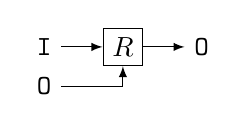
\begin{tikzpicture}[auto,>=latex]
      \node[] (I) {\code{I}};
      \node[below of=I, node distance=.5cm] (O) {\code{O}};
      \node[block, right of=I] (R) {$R$};
      \node[right of=R] (o) {\code{O}};
      \draw[->] (I) -- (R);
      \draw[->] (O) -| (R);
      \draw[->] (R) -- (o);
    \end{tikzpicture}
    \end{center}

\item Lift this circuit to operate on streams:
    \begin{center}
    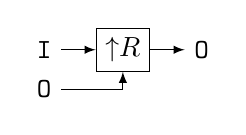
\begin{tikzpicture}[auto,>=latex]
      \node[] (I) {\code{I}};
      \node[below of=I, node distance=.5cm] (O) {\code{O}};
      \node[block, right of=I] (R) {$\lift R$};
      \node[right of=R] (o) {\code{O}};
      \draw[->] (I) -- (R);
      \draw[->] (O) -| (R);
      \draw[->] (R) -- (o);
    \end{tikzpicture}
    \end{center}
  We construct $\lift{R}$ by lifting each operator of the circuit individually
  according to Proposition~\ref{prop:distributivity}.

\item Build a cycle, connecting the output to the  corresponding
input via a delay:

 \begin{center}
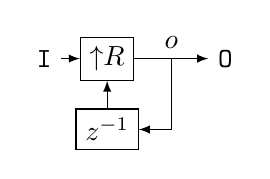
\begin{tikzpicture}[auto,>=latex, node distance=.8cm]
  \node[] (I) {\code{I}};
  \node[block, right of=I] (R) {$\lift R$};
  \node[right of=R, node distance=1.5cm] (O) {\code{O}};
  \node[block, below of=R, node distance=.9cm] (z) {$\zm$};
  \draw[->] (I) -- (R);
  \draw[->] (R) -- node(o) {$o$} (O);
  \draw[->] (o) |- (z);
  \draw[->] (z) -- (R);
 \end{tikzpicture}
 \end{center}
\item ``Bracket'' the circuit in $\I$ and $\D$ nodes, and then in $\delta_0$ and $\int$:

\begin{center}
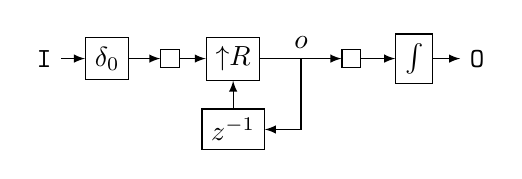
\begin{tikzpicture}[auto,>=latex, node distance=.8cm]
  \node[] (Iinput) {\code{I}};
  \node[block, right of=Iinput] (ID) {$\delta_0$};
  \node[block, right of=ID] (II) {$\I$};
  \node[block, right of=II] (f) {$\lift{R}$};
  \node[block, right of=f, node distance=1.5cm] (D) {$\D$};
  \node[block, right of=D] (S) {$\int$};
  \node[right of=S] (output)  {\code{O}};
  \draw[->] (Iinput) -- (ID);
  \draw[->] (ID) -- (II);
  \draw[->] (II) -- (f);
  \draw[->] (f) -- node (o) {$o$} (D);
  \draw[->] (D) -- (S);
  \draw[->] (S) -- (output);
  \node[block, below of=f, node distance=.9cm] (z) {$\zm$};
  \draw[->] (o) |- (z);
  \draw[->] (z) -- (f);
\end{tikzpicture}
\end{center}
\end{enumerate}
\end{algorithm}

This circuit as drawn is not a well-formed circuit.
\val{Why not well-formed? As far as I can see its semantics
follows from Corollary~\ref{feedback-semantics}.}
\mihai{The WFC rules require any circuit bracketed by $\delta_0$ -- $\int$ to have no other input or output edges.  It also
requires back-edges to go through a plus only.  It is
more strict than the stream computation rules.}
It can, however, be modified into an equivalent
well-formed circuit by adding two constant zero value streams:

\begin{center}
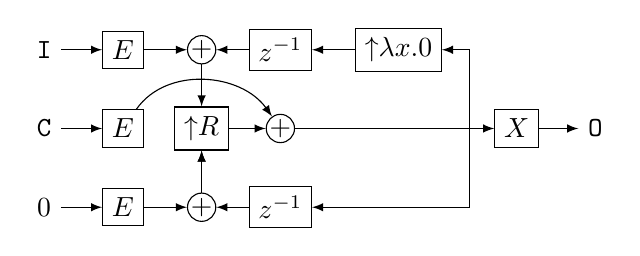
\begin{tikzpicture}[auto,>=latex]
  \node[] (Iinput) {\code{I}};
  \node[below of=Iinput] (Cinput) {\code{C}};
  \node[below of=Cinput] (Zinput) {$0$};
  \node[block, right of=Iinput] (IE) {$E$};
  \node[block, right of=Cinput] (CE) {$E$};
  \node[block, right of=Zinput] (ZE) {$E$};
  \node[block, shape=circle, right of=ZE, inner sep=0in] (Zplus) {$+$};
  \node[block, right of=CE] (f) {$\lift{R}$};
  \node[block, shape=circle, above of=f, inner sep=0in] (Cplus) {$+$};
  \node[block, right of=Cplus] (Cz) {$\zm$};
  \node[block, right of=Cz, node distance=1.5cm] (zero) {$\lift{\lambda x . 0}$};
  \node[block, right of=f, shape=circle, inner sep=0in] (plus) {$+$};
  \node[block, right of=plus, node distance=3cm] (X) {$X$};
  \node[right of=X] (output)  {\code{O}};
  \node[block, below of=plus] (z) {$\zm$};

  \draw[->] (Iinput) -- (IE);
  \draw[->] (Cinput) -- (CE);
  \draw[->] (Zinput) -- (ZE);
  \draw[->] (ZE) -- (Zplus);
  \draw[->] (CE) to[out=55,in=125] (plus);
  \draw[->] (plus) -- +(right:2.4cm) node (o) {} -- (X);
  \draw[->] (X) -- (output);
  \draw[->] (o.south) |- (zero);
  \draw[->] (Zplus) -- (f);
  \draw[->] (z) -- (Zplus);
  \draw[->] (Zplus) -- (f);
  \draw[->] (IE) -- (Cplus);
  \draw[->] (f) -- (plus);
  \draw[->] (zero) -- (Cz);
  \draw[->] (o) |- (z);
  \draw[->] (Cz) -- (Cplus);
  \draw[->] (Cplus) -- (f);
\end{tikzpicture}
\end{center}

\begin{theorem}
If $\isset(\code{I})$ and $\isset(\code{C})$, the output of the circuit above is
the relation $\code{O}$ as defined by the Datalog semantics of recursive relations
as a function of the input relations \code{I} and \code{C}.
\end{theorem}

\begin{proof}
The proof is by structural induction on the structure of the circuit.
As a basis for induction we assume that the circuit $R$ correctly implements
the semantics of the recursive rule body when treating \code{O} as an
independent input.  We need to prove that the output of circuit encompassing
$R$ produces the correct value of the \code{O} relation, as defined by
the recursive Datalog equation.

Let us compute the contents of the $o$ stream, produced at the output
of the $\distinct$ operator.  We will show that this stream is composed
of increasing approximations of the value of \code{O}, and in fact
$\code{O} = \lim_{t \to \infty} o[t]$ if the limit exists.

We define the following one-argument function: $R'(x) = \lambda x . R(\code{I}, x)$.
Notice that the left input of the $\lift{R}$ block is a constant stream
with the value \code{I}.  Due to the stratified nature of the language,
we must have $\ispositive(R')$, so $\forall x . R'(x) \geq x$.
Also $\lift{R'}$ is time-invariant, so $R'(0) = 0$.

With this notation for $R'$ the previous circuit has the
output as the following simpler circuit:

\begin{center}
\begin{tikzpicture}[auto,>=latex]
  \node[] (Cinput) {\code{C}};
  \node[block, right of=Cinput] (CE) {$E$};
  \node[block, below of=CE] (f) {$\lift{R'}$};
  \node[block, right of=f, shape=circle, inner sep=0in] (plus) {$+$};
  \node[block, right of=plus, node distance=1.5cm] (X) {$X$};
  \node[right of=X] (output)  {\code{O}};
  \draw[->] (Cinput) -- (CE);
  \draw[->] (f) -- (plus);
  \draw[->] (plus) -- node (o) {$o$} (X);
  \draw[->] (X) -- (output);
  \node[block, below of=plus] (z) {$\zm$};
  \draw[->] (o) |- (z);
  \draw[->] (z) -| (f);
  \draw[->] (CE) -| (plus);
\end{tikzpicture}
\end{center}

We use the following notation: $x \cup y = \distinct(x + y)$.  As discussed in Section~\ref{sec:union}
the $\cup$ operation computes the same result as set union when $x$ and $y$ are sets.
With this notation let us compute the values of the $o$ stream:

$$
\begin{aligned}
o[0] =& \code{C} + R'(0) = \code{C} \cup R'(0) = \code{C} \\
o[1] =& \code{C} + R'(o[0]) = \code{C} \cup R'(\code{C}) \\
o[t] =& \code{C} + R(o[t-1]) = \code{C} \cup R'(o[t-1]) \\
\end{aligned}
$$

Defining a new helper function $S(x) = \code{C} \cup R'(x)$, the previous system of equations becomes:

$$
\begin{aligned}
o[0] =& S(0) \\
o[1] =& S(S(0)) \\
o[t] =& S(o[t-1]) \\
\end{aligned}
$$

So, by induction $o[t] = S^t(0)$, where by $S^t$ we mean $\underbrace{S \circ S \circ \ldots \circ S}_{t}$.
$S$ is monotone because $R'$ is monotone; thus, if there is a time $k$ such that $S^k(0) = S^{k+1}(0)$, we have
$\forall j \in \N . S^{k+j}(0) = S^k(0)$.

\code{O} is computed by the $X$ operator as the limit of stream $o$:
$\code{O} = X(o) = \lim_{n \to \infty} o[n]$.  If this limit exists (i.e., a fixed-point
is reached), the circuit computes the fixed point $\fix{x}{S(x)}$.  This is exactly
the definition of the Datalog semantics of a recursive relation definition: $\code{O} =
\fix{x}{\code{C} \cup R(\code{I}, x)}$.
\end{proof}

Note that the use of unbounded domains (like integers with arithmetic operations) does
not guarantee convergence for all programs.

Our circuit implementation is in fact computing the value of relation \code{O} using the standard
\defined{na\"{\i}ve evaluation} algorithm (e.g., see Algorithm~1 from \cite{greco-sldm15}).

Observe that the ``inner'' part of the circuit is the incremental
form of another circuit, since is ``sandwiched'' between $\I$ and $\D$ operators.
According to Proposition~\ref{prop-inc-properties}, part 7, the circuit can be
rewritten as:

\begin{equation}
\begin{aligned}
  \label{eq:seminaive}
\begin{tikzpicture}[auto,>=latex]
  \node[] (Cinput) {\code{C}};
  \node[below of=Cinput] (Iinput) {\code{I}};
  \node[block, right of=Iinput] (Idelta) {$\delta_0$};
  \node[block, above of=Idelta] (Cdelta) {$\delta_0$};
  \node[block, right of=Idelta] (f) {$\inc{\lift{R}}$};
  \node[block, right of=f, shape=circle, inner sep=0in] (plus) {$+$};
  \node[block, right of=plus, node distance=1.5cm] (S) {$\int$};
  \node[right of=S] (output)  {\code{O}};
  \node[block, below of=plus] (z) {$\zm$};
  \draw[->] (Iinput) -- (Idelta);
  \draw[->] (Cinput) -- (Cdelta);
  \draw[->] (Cdelta) -| (plus);
  \draw[->] (f) -- (plus);
  \draw[->] (plus) -- node (o) {} (S);
  \draw[->] (S) -- (output);
  \draw[->] (o) |- (z);
  \draw[->] (z) -| (f);
  \draw[->] (Idelta) -- (f);
\end{tikzpicture}
\end{aligned}
\end{equation}

This form of the circuit is effectively implementing the \defined{semi-na\"{\i}ve evaluation}
of the same relation (Algorithm~2 from~\cite{greco-sldm15}).  So the correctness of semi-na\"{\i}ve evaluation
is an immediate consequence of the cycle rule from Proposition~\ref{prop-inc-properties}.

\begin{comment}
Let us notice that the combination $\int \circ \D$ applied to a
monotone stream will produce that fixed-point value of the input
stream (if it exists).  This suggests a simple practical implementation
for for $\int$ operator: stop aggregating at the first input that is 0.
For monotone loop bodies involving a positive query $Q$ this implementation is
correct.
\end{comment}

\subsection{Example: a recursive query in \dbsp}\label{sec:recursive-example}

Here we apply the algorithm~\ref{algorithm-rec}, that converts a
recursive query into a DBSP circuit, to a concrete Datalog program.
The program computes the transitive closure of a directed graph:

\begin{lstlisting}[language=ddlog,basicstyle=\small]
// Edge relation with head and tail
input relation E(h: Node, t: Node)
// Reach relation with source s and sink t
output relation R(s: Node, t: Node)
R(x, y) :- E(x, y).
R(x, y) :- E(x, z), R(z, y).
\end{lstlisting}

Step 1: we ignore the fact that R is both an input and an output and we implement
the \dbsp circuit corresponding to the body of the query.  This query could be expressed
in SQL as:

\begin{lstlisting}[language=SQL,basicstyle=\small]
( SELECT * FROM E)
UNION
( SELECT E.h , R.t
  FROM E JOIN R
  ON E.t = R.s )
\end{lstlisting}

This query generates a \dbsp circuit with inputs \code{E} and \code{R}:

\begin{center}
\begin{tikzpicture}[>=latex, node distance=1.2cm]
  \node[] (E) {\code{E}};
  \node[above of=E, node distance=.8cm] (R1) {\code{R}};
  \node[block, right of=R1] (j) {$\bowtie_{t=s}$};
  \node[block, right of=j] (pj) {$\pi_{h, t}$};
  \node[block, circle, below of=pj, inner sep=0cm, node distance=.8cm] (plus) {$+$};
  \node[block, right of=plus] (d) {$\distinct$};
  \node[right of=d] (R) {\code{R}};
  \draw[->] (R1) -- (j);
  \draw[->] (E) -- (j);
  \draw[->] (j) -- (pj);
  \draw[->] (E) -- (plus);
  \draw[->] (pj) -- (plus);
  \draw[->] (plus) -- (d);
  \draw[->] (d) -- (R);
\end{tikzpicture}
\end{center}

Step 2: Lift the circuit by lifting each operator pointwise:

\begin{center}
\begin{tikzpicture}[>=latex, node distance=1.5cm]
  \node[] (E) {\code{E}};
  \node[above of=E, node distance=.9cm] (R1) {\code{R}};
  \node[block, right of=R1] (j) {$\lift{\bowtie_{t=s}}$};
  \node[block, right of=j] (pj) {$\lift{\pi_{h, t}}$};
  \node[block, circle, below of=pj, node distance=.9cm, inner sep=0cm] (plus) {$+$};
  \node[block, right of=plus] (d) {$\lift{\distinct}$};
  \node[right of=d] (R) {\code{R}};
  \draw[->] (R1) -- (j);
  \draw[->] (E) -- (j);
  \draw[->] (j) -- (pj);
  \draw[->] (E) -- (plus);
  \draw[->] (pj) -- (plus);
  \draw[->] (plus) -- (d);
  \draw[->] (d) -- (R);
\end{tikzpicture}
\end{center}

Step 3: Connect the feedback loop implied by relation \code{R}:

\begin{center}
\begin{tikzpicture}[>=latex]
  \node[] (E) {\code{E}};
  \node[right of=E] (empty) {};
  \node[block, above of=empty, node distance=.8cm] (j) {$\lift{\bowtie_{t=s}}$};
  \node[block, right of=j, node distance=1.4cm] (pj) {$\lift{\pi_{h, t}}$};
  \node[block, circle, below of=pj, node distance=.8cm, inner sep=0cm] (plus) {$+$};
  \node[block, right of=plus, node distance=1.3cm] (d) {$\lift{\distinct}$};
  \draw[->] (E) -- (j);
  \draw[->] (j) -- (pj);
  \draw[->] (E) -- (plus);
  \draw[->] (pj) -- (plus);
  \draw[->] (plus) -- (d);

  % generic part
  \node[right of=d, node distance=1.4cm] (output)  {\code{R}};
  \draw[->] (d) -- node (o) {} (output);
  \node[block, above of=j, node distance=.8cm] (z) {$\zm$};
  \draw[->] (o.center) |- (z);
  \draw[->] (z) -- (j);
\end{tikzpicture}
\end{center}

Step 4: ``bracket'' the circuit, once with $\I$-$\D$, then with $\delta_0$-$\int$:

\noindent
\begin{equation}\label{recursive-join}
\begin{tikzpicture}[>=latex]
  \node[] (Einput) {\code{E}};
  % generic part
  \node[block, right of=Einput, node distance=.8cm] (ID) {$\delta_0$};
  \node[block, right of=ID, node distance=.8cm] (E) {$\I$};

  % relational query
  \node[block, above of=E, node distance=.8cm] (j) {$\lift{\bowtie_{t=s}}$};
  \node[block, right of=j, node distance=1.5cm] (pj) {$\lift{\pi_{h, t}}$};
  \node[block, circle, below of=pj, node distance=.8cm, inner sep=0cm] (plus) {$+$};
  \node[block, right of=plus, node distance=1.3cm] (d) {$\lift{\distinct}$};
  \draw[->] (E) -- (j);
  \draw[->] (j) -- (pj);
  \draw[->] (E) -- (plus);
  \draw[->] (pj) -- (plus);
  \draw[->] (plus) -- (d);

  % generic part
  \node[block, right of=d, node distance=1.3cm] (D) {$\D$};
  \node[block, right of=D, node distance=.8cm] (S) {$\int$};
  \node[right of=S, node distance=.8cm] (output)  {\code{R}};
  \draw[->] (Einput) -- (ID);
  \draw[->] (ID) -- (E);
  \draw[->] (d) -- node (o) {} (D);
  \draw[->] (D) -- (S);
  \draw[->] (S) -- (output);
  \node[block, above of=j, node distance=.8cm] (z) {$\zm$};
  \draw[->] (o.center) |- (z);
  \draw[->] (z) -- (j);
\end{tikzpicture}
\end{equation}

The above circuit is a complete implementation of the non-streaming
recursive query; given an input relation \code{E} it will produce
its transitive closure \code{R} at the output.

Now we use semina\"ive evaluation~\ref{eq:seminaive} to rewrite the circuit
(to save space in the figures we will omit the indices from $\pi$ and $\sigma$
in the subsequent figures):

\begin{center}
\begin{tikzpicture}[>=latex, node distance=1.4cm]
  \node[] (Einput) {\code{E}};
  % generic part
  \node[block, right of=Einput, node distance=.8cm] (E) {$\delta_0$};

  % relational query
  \node[block, above of=E, node distance=.9cm] (j) {$\inc{(\lift{\bowtie})}$};
  \node[block, right of=j, node distance=1.5cm] (pj) {$\inc{(\lift{\pi})}$};
  \node[block, circle, below of=pj, node distance=.9cm, inner sep=0cm] (plus) {$+$};
  \node[block, right of=plus, node distance=1.5cm] (d) {$\inc{(\lift{\distinct})}$};
  \draw[->] (E) -- (j);
  \draw[->] (j) -- (pj);
  \draw[->] (E) -- (plus);
  \draw[->] (pj) -- (plus);
  \draw[->] (plus) -- (d);

  % generic part
  \node[block, right of=d, node distance=1.6cm] (S) {$\int$};
  \node[right of=S, node distance=1cm] (output)  {\code{R}};
  \draw[->] (Einput) -- (E);
  \draw[->] (d) -- node (o) {} (S);
  \draw[->] (S) -- (output);
  \node[block, above of=j, node distance=.9cm] (z) {$\zm$};
  \draw[->] (o.center) |- (z);
  \draw[->] (z) -- (j);
\end{tikzpicture}
\end{center}

Using the linearity of $\lift\pi$, this can be rewritten as:

\begin{center}
\begin{tikzpicture}[>=latex, node distance=1.3cm]
  \node[] (Einput) {\code{E}};
  % generic part
  \node[block, right of=Einput, node distance=.8cm] (E) {$\delta_0$};

  % relational query
  \node[block, above of=E, node distance=.9cm] (j) {$\inc{(\lift{\bowtie})}$};
  \node[block, right of=j] (pj) {$\lift{\pi}$};
  \node[block, circle, below of=pj, node distance=.9cm, inner sep=0cm] (plus) {$+$};
  \node[block, right of=plus, node distance=1.6cm] (d) {$\inc{(\lift{\distinct})}$};
  \draw[->] (E) -- (j);
  \draw[->] (j) -- (pj);
  \draw[->] (E) -- (plus);
  \draw[->] (pj) -- (plus);
  \draw[->] (plus) -- (d);

  % generic part
  \node[block, right of=d, node distance=1.6cm] (S) {$\int$};
  \node[right of=S, node distance=.8cm] (output)  {\code{R}};
  \draw[->] (Einput) -- (E);
  \draw[->] (d) -- node (o) {} (S);
  \draw[->] (S) -- (output);
  \node[block, above of=j, node distance=.9cm] (z) {$\zm$};
  \draw[->] (o.center) |- (z);
  \draw[->] (z) -- (j);
\end{tikzpicture}
\end{center}

\subsubsection{Mutually recursive rules}\label{sec:mutually-recursive}

Given a stratified Datalog program we can compute a graph where relations are nodes and dependences
between relations are edges.  We then compute the strongly connected components of this graph.
All relations from a strongly-connected component are mutually recursive.

Let us consider the implementation of a single strongly-connected component defining $n$
relations $O_i, i \in [n]$.  We can assume wlog that the definition of $O_i$ has the following
structure:
\newcommand{\tns}{\code{:-}}
\newcommand{\cd}{\code{.}}
$$
\begin{array}{lll}
O_i(v) &\tns& C_i(v)\cd \\
O_i(v) &\tns&  I_i(x), O_0(v_0), O_1(v_1), \ldots, O_{n-1}(v_{n-1}), v = \ldots \cd \\
\end{array}
$$

There are exactly $n$ base cases, one defining each $O_i$.  Also, we assume that each $O_i$ relation
depends on an external relation $I_i$, which does not itself depend on any $O_k$.

To compile these into circuits we generalize the algorithm from Section~\ref{sec:recursion}:

\begin{enumerate}
    \item For each recursive rule for $O_i$ implement a circuit $R_i$
    that treats all $O_j . j \in [n]$ and $I_i$ in the rule body as inputs.
    Here is the circuit $R_0$ for relation $O_0$:

    \begin{tikzpicture}[auto,>=latex]
      \node[] (i) {$I_0$};
      \node[below of=i, node distance=.7cm] (o0) {$O_0$};
      \node[below of=o0, node distance=.3cm] (odots) {$\ldots$};
      \node[below of=odots, node distance=.3cm] (on) {$O_{n-1}$};
      \node[block, right of=i, node distance=2cm] (R) {$R_0$};
      \node[right of=R] (output) {};
      \draw[->] (o0) -- (R);
      \draw[->] (on) -- (R);
      \draw[->] (i) -- (R);
      \draw[->] (R) -- (output);
    \end{tikzpicture}

    \item Embed each circuit $R_i$ as part of a ``widget'' as follows:

    \begin{tikzpicture}[auto,>=latex]
      \node[] (c0) {$C_0$};
      \node[below of=c0, node distance=.7cm] (i) {$I_0$};
      \node[below of=i, node distance=.7cm] (o0) {$O_0$};
      \node[below of=o0, node distance=.3cm] (odots) {$\ldots$};
      \node[below of=odots, node distance=.3cm] (on) {$O_{n-1}$};
      \node[block, right of=i, node distance=2cm] (R) {$R_0$};
      \node[block, right of=R, shape=circle, inner sep=0in] (plus) {$+$};
      \node[right of=plus, node distance=1.5cm] (o) {$O_0'$};
      \draw[->] (o0) -- (R);
      \draw[->] (on) -- (R);
      \draw[->] (i) -- (R);
      \draw[->] (R) -- (plus);
      \draw[->] (plus) -- (o);
      \draw[->] (c0) -| (plus);
    \end{tikzpicture}

    \item Finally, lift each such widget and connect them to each other via
    $\zm$ operators to the corresponding recursive inputs.
    The following is the shape of the circuit computing $O_0$;
    the $O_j'$ sources correspond to the widget outputs of the other
    recursive circuits:

    \begin{tikzpicture}[auto,>=latex]
      \node[] (c0) {$C_0$};
      \node[block, right of=c0] (ec0) {$E$};
      \node[below of=c0, node distance=.7cm] (i) {$I_0$};
      \node[block, right of=i] (ei) {$E$};
      \node[right of=ei] (marker) {};
      \node[block, below of=marker, node distance=.7cm] (z0) {$\zm$};
      \node[below of=z0, node distance=.35cm] (dots) {$\ldots$};
      \node[block, below of=dots, node distance=.35cm] (zn) {$\zm$};
      \node[block, right of=ei, node distance=2.5cm] (R) {$\lift{R_0}$};
      \node[block, right of=R, shape=circle, inner sep=0in] (plus) {$+$};
      \node[block, right of=plus, node distance=2cm] (X) {$X$};
      \node[right, right of=X] (o) {$O_0$};
      \node[right of=zn, node distance=4cm] (on) {$O_{n-1}'$};

      \draw[->] (c0) -- (ec0);
      \draw[->] (i) -- (ei);
      \draw[->] (ei) -- (R);
      \draw[->] (R) -- (plus);
      \draw[->] (plus) -- node (oo) {$O_o'$} (X);
      \draw[->] (ec0) -| (plus);
      \draw[->] (X) -- (o);
      \draw[->] (oo) |- (z0);
      \draw[->] (on) -- (zn);
      \draw[->] (z0) -- (R);
      \draw[->] (zn) -- (R);
    \end{tikzpicture}
\end{enumerate}

\begin{theorem}
The program defined by the previous circuit computes
the relations $O_i$ as a function of the input relations $I_j$ and $C_i$.
\end{theorem}
\begin{proof}
TODO.
\end{proof}

\paragraph{Example: mutually recursive relations}

Consider the Datalog program below computing the transitive closure of a graph
having two kinds of edges, blue (B) and red (R):

\begin{lstlisting}[language=ddlog]
P(x,y) :- B(x,y).
Q(x,y) :- R(x,y).
P(x,y) :- B(x,z), Q(z,y).
Q(z,y) :- R(x,z), P(z,y).
O(x,y) :- P(x,y).
O(x,y) :- Q(x,y).
\end{lstlisting}

The program defined by the following circuit computes
the relation $\code{O}$ as a function of the input relations $\code{R}, \code{B}$:

\val{I will add in Section~\ref{sec:causal} a consequence of Corollary~\ref{feedback-semantics} to justify the well-definedness of this.}

\begin{center}
\begin{tikzpicture}[auto,>=latex]
\node[] (inputB) {\code{B}};
\node[block, right of=inputB] (EB) {$E$};

\node[block, shape=circle, right of=EB, node distance=1.5cm, inner sep=0in] (plusP) {$+$};
\node[block, right of=plusP, node distance=1.5cm] (distinctP) {$\lift{\distinct}$};
\node[block, below of=distinctP] (zP) {$\zm$};
\node[block, below of=zP] (zQ) {$\zm$};
\node[block, below of=zQ] (distinctQ) {$\lift{\distinct}$};
\node[block, right of=distinctP, node distance=1.5cm] (xP) {$X$};
\node[block, right of=distinctQ, node distance=1.5cm] (xQ) {$X$};

\node[block, shape=circle, left of=distinctQ, node distance=1.5cm, inner sep=0in] (plusQ) {$+$};
\node[block, left of=zP, node distance=1.5cm] (joinP) {$\lift{\bowtie}$};
\node[block, left of=zQ, node distance=1.5cm] (joinQ) {$\lift{\bowtie}$};

\node[block, left of=plusQ, node distance=1.5cm] (ER) {$E$};
\node[left of=ER] (inputR) {\code{R}};

\path (xP) -- node[block, shape=circle, inner sep=0cm] (sum) {$+$} (xQ);
\node[right of=sum] (O) {\code{O}};
\path (inputB) -- (inputR) ;

\draw[->] (inputB) -- (EB);
\draw[->] (inputR) -- (ER);
\draw[->] (EB) -- (plusP);
\draw[->] (ER) -- (plusQ);
\draw[->] (plusP) -- (distinctP);
\draw[->] (plusQ) -- (distinctQ);
\draw[->] (zP) -- (joinQ);
\draw[->] (zQ) -- (joinP);
\draw[->] (EB) -- (joinP);
\draw[->] (ER) -- (joinQ);
\draw[->] (joinQ) -- (plusQ);
\draw[->] (joinP) -- (plusP);
\draw[->] (distinctP) -- (zP);
\draw[->] (distinctQ) -- (zQ);
\draw[->] (distinctP) -- (xP);
\draw[->] (distinctQ) -- (xQ);
\draw[->] (xP) -- node (p) {\code{P}} (sum);
\draw[->] (xQ) -- node (q) [right] {\code{Q}} (sum);
\draw[->] (sum) -- (O);
\end{tikzpicture}
\end{center}

\section{Additional query languages}\label{sec:extensions}

In this section we describe several query models that go behind stratified Datalog
and show how they can be implemented in \dbsp.

\subsection{Aggregation}\label{sec:aggregation}

Aggregation in SQL applies a function $a$ to a whole set producing a ``scalar''
result with some type $R$: $a: 2^A \to R$.  We convert such aggregation
functions to operate on \zrs, so in \dbsp an aggregation function has
a signature $a: \Z[A] \to R$.  Correctness of the implementation is 
defined as in \refsec{sec:correctness}.

The SQL \texttt{COUNT} aggregation function is implemented on \zrs by $a_\texttt{COUNT} : \Z[A] \to \Z$, which
computes a \emph{sum} of all the element weights: $a_\texttt{COUNT}(s) = \sum_{x \in s} s[x]$.
The SQL \texttt{SUM} aggregation function is implemented on \zrs by $a_\texttt{SUM}: \Z[\R] \to \R$ which
performs a \emph{weighted sum} of all (real) values: $a_\texttt{SUM}(s) = \sum_{x \in s} x \times s[x]$.

With this definition the aggregation functions $a_\texttt{COUNT}$ and $a_\texttt{SUM}$ are in
fact linear transformations between the group $\Z[A]$ and the result group ($\Z$, and $\R$ respectively).

If the output of the \dbsp circuit can be such a ``scalar'' value, then aggregation
with a linear function is simply function application, and thus it is automatically incremental.  However, in general, for composing multiple queries
we require the result of an aggregation to be a singleton \zr (containing a single value),
and not a scalar value.  In this case the aggregation function is implemented in
\dbsp as the composition of the actual aggregation and the 
$\makeset: A \to \Z[A]$ function, 
which converts a scalar value of type $A$ to a singleton \zr, defined as follows:
$\makeset(x) \defn 1 \cdot x$.

In conclusion, the following SQL query: 
\code{SELECT SUM(c) FROM I} 
is implemented as the following circuit:

\begin{tikzpicture}[auto,>=latex]
  \node[] (I) {\code{I}};
  \node[block, right of=I] (pi) {$\pi_\texttt{C}$};
  \node[block, right of=pi] (a) {$a_\texttt{SUM}$};
  \draw[->] (I) -- (pi);
  \draw[->] (pi) -- (a);
  \node[block, right of=a, node distance=1.5cm] (m) {$\makeset$};
  \node[right of=m, node distance=1.4cm] (O) {\code{O}};
  \draw[->] (a) -- (m);
  \draw[->] (m) -- (O); 
\end{tikzpicture}

The lifted incremental version of this circuit is interesting: since $\pi$ 
and $a_\texttt{SUM}$ are linear, they are equivalent to their own incremental 
versions.  Although $\inc{(\lift \makeset)} = \D \circ \lift{\makeset} \circ \I$
cannot be simplified, it is nevertheless efficient, doing only O(1) work per
invocation, since its input and output are singleton values.

An aggregation function such as \texttt{AVG} can be written as the composition of 
a more complex linear function that computes a pair of values using 
\texttt{SUM} and \texttt{COUNT}, followed by a $\mbox{makeset}$ and a selection operation
that divides the two columns.

\begin{lstlisting}[language=SQL]
SELECT AVG(c) FROM I 
\end{lstlisting}

\begin{tikzpicture}[>=latex]
  \node[] (I) {\code{I}};
  \node[block, right of=I] (pi) {$\pi_\texttt{C}$};
  \node[block, right of=pi, node distance=1.8cm] (sc) {$(a_\texttt{SUM}, a_\texttt{COUNT})$};
  \draw[->] (I) -- (pi);
  \draw[->] (pi) -- (sc);
  \node[block, right of=sc, node distance=2cm] (m) {$\makeset$};
  \node[block, right of=m, node distance=1.4cm] (div) {$\sigma_/$};
  \node[right of=div] (O) {\code{O}};
  \draw[->] (sc) -- (m);
  \draw[->] (m) -- (div);
  \draw[->] (div) -- (O);
\end{tikzpicture}

Finally, some aggregate functions, such as \code{MIN}, are 
\emph{not} incremental in general, since for handling deletions
they may need to know the full set, and not just its changes.  The lifted
incremental version of such aggregate functions is implemented essentially
by ``brute force'', using the formula $\inc{(\lift a_\texttt{MIN})}
= \D \circ \lift{a_\texttt{MIN}} \circ \I$.  Such functions perform work
proportional to $R(s)$ at each invocation.

Note that the SQL \code{ORDER BY} directive can be modeled as
a non-linear aggregate function that emits a list.  However, such an implementation it is not efficiently incrementalizable in \dbsp. 
We leave the efficient handling of ORDER BY to future work.

Even when aggregation results do not form a group, they usually form
a structure with a zero element.  We expect that a well-defined
aggregation function maps empty \zrs to zeros in the target domain.


\subsection{Nested relations}

\subsubsection{Indexed partitions}

Let $A[K]$ be the set of functions with finite support from $K$ to $A$.
Consider a group $A$, an arbitrary set of \defined{key values} $K$, and a 
\emph{partitioning function} $k: A \to A[K]$ with the property that 
$\forall a \in A . a = \sum k(a)$.  We call elements of $A[K]$ \emph{indexed}
values of $A$ --- indexed by a key value.

Notice that $A[K]$ also has a group structure, and $k$ itself 
is a linear function (homomorphism).  As an example,
if $A = \Z[B_0 \times B_1]$, we can use for $k$ the first projection
$k: A \to \Z[A][B_0]$, where $k(a)[b] = \sum_{t \in a, t|0 = b} a[t] \cdot t$.
In other words, $k$ projects the elements in $\Z[B_0 \times B_1]$ on 
their first component.  This enables \emph{incremental computations
on nested relations}.  This is how operators such as group-by are
implemented: the result of group-by is an indexed \zr, where each 
element is indexed by the key of the group it belongs to.  Since
indexing is linear, its incremental version is very efficient.
Notice that the structure $\Z[A][K]$ represents a form of \emph{nested relation}.

\subsection{Grouping; indexed relations}\label{sec:grouping}

Pick an arbitrary set $K$ of ``key values.''
Consider the mathematical structure of finite maps from $K$ 
to \zrs over some other domain $A$: $K \to \Z[A] = \Z[A][K]$.
We call values $i$ of this structure \defined{indexed \zrs}: for
each key $k \in K$, $i[k]$ is a \zr.  Because 
the codomain $\Z[A]$ is an abelian group, this structure is itself 
an abelian group.

We use this structure to model the SQL \texttt{GROUP BY} operator in \dbsp.  
Consider a \defined{partitioning function}
$p: A \to K$ that assigns a key to any value in $A$.  We define the grouping function
$G_p: \Z[A] \to (K \to \Z[A])$ as $G_p(a)[k] \defn \sum_{x \in a.p(x)=k}a[x] \cdot x$.
When applied to a \zr $a$ this function returns a indexed \zr, where each element 
is called a \defined{grouping}\footnote{We use
``group'' for the algebraic structure and ``grouping'' for the result of \code{GROUP BY}.}: for each key $k$ a 
grouping is a \zr containing all elements of $a$ that map to $k$ 
(as in SQL, groupings are multisets, represented by \zrs).
Consider our example \zr $R$ from \refsec{sec:relational},
and a key function $p(s)$ that returns the first letter of the string 
$s$. Then we have that $G_p(R) = \{ \code{j} \mapsto \{ \code{joe} 
\mapsto 1 \}, \code{a} \mapsto \{ \code{anne} \mapsto -1 \} \}$,
i.e., grouping with this key function produces an indexed \zr with two groupings, each 
of which contains a \zr with one element.

The grouping function $G_p$ is linear for any $p$.
It follows that the group-by implementation in DBSP is automatically
incremental: given some changes
to the input relation we can apply the partitioning function
to each change separately to compute how each grouping changes.

\subsection{\texttt{GROUP BY-AGGREGATE}}

Grouping in SQL is almost always followed by aggregation.  
Let us consider an aggregation function $a: (K \times \Z[A]) \to B$ that produces values
in some group $B$, and an indexed relation of type $\Z[A][K]$, as defined above in~\refsec{sec:grouping}.
The nested relation aggregation operator $Agg_a: \Z[A][K] \to B$ applies $a$ 
to the contents of each grouping independently and adds the results:
$Agg_a(g) \defn \sum_{k \in K} a(k, g[k])$.  To apply this
to our example, let us compute the equivalent of GROUP-BY count; we use
the following aggregation function $count: K \times \Z[A]$, $count(k, s) = 
\makeset((k, a_\texttt{COUNT}(s)))$, using the \zr counting function $a_\texttt{COUNT}$ 
from~\refsec{sec:aggregation}; the notation $(a,b)$ is a pair of values $a$ and $b$.
Then we have $Agg_{count} (G_p(R)) = \{ (\code{j}, 1) \mapsto 1, 
(\code{a}, -1) \mapsto 1 \}$.

Notice that, unlike SQL, \dbsp can express naturally computations
on indexed \zrs, they are just an instance of a group structure. 
One can even implement queries that operate on each grouping 
in an indexed \zr.  However, our definition of incremental 
computation is only concerned with incrementality in the 
\emph{outermost} structures.  We leave it to future work to
explore an appropriate definition of incremental computation that
operates on the \emph{inner} relations.

A very useful operation on nested relations is \defined{flatmap}, which is
essentially the inverse of partitioning, converting an indexed
\zr into a \zr: $\mbox{flatmap}: \Z[A][K] \to \Z[A \times K]$.
$\mbox{flatmap}$ is in fact a particular instance of aggregation,
using the aggregation function $a: K \times \Z[A] \to \Z[A \times K]$
defined by $a(k, s) = \sum_{x \in s[k]} s[k][x] \cdot (k, x).$
For our previous example, $\mbox{flatmap}(G_p(R)) = \{ (\code{j}, \code{joe}) \mapsto 1, 
(\code{a}, \code{anne}) \mapsto -1 \}$.

If we use an aggregation function $a: K \times Z[A]$ that is linear in its
second argument, then the aggregation operator $Agg_a$ is linear, and
thus fully incremental.  As a consequence, $\mbox{flatmap}$ is linear.  
However, many practical aggregation functions for nested relations are in fact 
not linear; an example is the $count$ function above, which is not linear
since it uses the $\makeset$ non-linear function.  Nevertheless, while 
the incremental evaluation of such functions is not fully incremental, 
it is at least partly incremental: when applying a change to groupings, the aggregation 
function only needs to be re-evaluated \emph{for groupings that have changed}.


\subsection{Streaming joins}

Consider a binary query $T(s, t) = \I(t)~~\lift{\bowtie}~~s$.  This is the
\emph{relation-to-stream join} operator supported by streaming databases like ksqlDB~\cite{jafarpour-edbt19}.
Stream $t$ carries changes to a relation, while $s$ carries arbitrary data, e.g., logs
or telemetry data points. $T$ ``discards'' values from $s$ after matching them against the accumulated contents of the relation.

\begin{center}
\noindent
\begin{tikzpicture}[>=latex]
  \node[] (t) {$t$};
  \node[below of=t] (s) {$s$};
  \node[right of=t, block] (I) {$\I$};
  \node[below of=t, node distance=.5cm] (mid) {};
  \node[block, right of=mid, node distance=2cm] (j) {$\bowtie$};
  \node[right of=j] (o) {$o$};
  \draw[->] (s) -| (j);
  \draw[->] (t) -- (I);
  \draw[->] (I) -| (j);
  \draw[->] (j) -- (o);
\end{tikzpicture}
\end{center}

\subsection{Explicit delay}

So far the $\zm$ operator was confined to its implicit use in integration or
differentiation.  However, it can be exposed as a primitive operation that
can be applied to streams or collections.  This enables programs that can
perform time-based window computations over streams, and convolution-like
operators.  


\subsection{Multisets/bags}

Since \zrs generalize multisets and bags, it is easy to implement query
operators that compute on such structures.  For example, while SQL \code{UNION}
is \zr addition followed by $\distinct$, \code{UNION ALL} is just \zr addition.


\subsection{Window aggregates}

Streaming databases often organize the contents of streams into windows, 
which store a subset of data points with a predefined range of timestamps.
The circuit below (a convolution filter in DSP) computes a \emph{fixed-size sliding-window aggregate}
over the last four timestamps defined by the $T_i$ functions.

\begin{center}
\begin{tikzpicture}[>=latex]
    \node[] (input) {$s$};
    \node[block, right of=input, node distance=1.5cm] (f0) {$T_0$};
    \node[below of=input, node distance=1cm] (fake) {};
    \node[block, right of=fake, node distance=1cm] (z0) {$\zm$};
    \node[right of=input, node distance=.35cm] (tap) {};
    \node[block, right of=f0, node distance=1.5cm] (f1) {$T_1$};
    \node[block, right of=z0, node distance=1.2cm] (z1) {$\zm$};
    \node[block, right of=f1, node distance=1.5cm] (f2) {$T_2$};
    \node[block, right of=z1, node distance=1.5cm] (z2) {$\zm$};
    \draw[->] (input) -- (f0);
    \draw[->] (tap.center) |- (z0);
    \draw[->] (z0) -| (f0);
    \draw[->] (f0) -- (f1);
    \draw[->] (z0) -- (z1);
    \draw[->] (z1) -| (f1);
    \draw[->] (f1) -- (f2);
    \draw[->] (z1) -- (z2);
    \draw[->] (z2) -| (f2);
    \node[right of=f2] (output) {$o$};
    \draw[->] (f2) -- (output);
\end{tikzpicture}
\end{center}

In practice, windowing is usually based on physical timestamps attached to
stream values rather than logical time.  For instance, the CQL~\cite{arasu-tr02} query
``\texttt{SELECT * FROM events [RANGE 1 hour]}'' returns all events received
within the last hour.  The corresponding circuit (on the left) takes input stream $s \in \stream{\Z[A]}$ and an additional
input $\theta \in \stream{\mathbb{R}}$ that carries the value of the current
time.

\begin{tabular}{m{3cm}m{0.5cm}m{3cm}}
\begin{tikzpicture}[>=latex]
    \node[] (input) {$s$};
    \node[above of=input, node distance=.5cm] (t) {$\theta$};
    \node[block, right of=input] (i) {$I$};
    \node[block, right of=i] (w) {$W$};
    \node[right of=w] (output) {$o$};
    \draw[->] (input) -- (i);
    \draw[->] (i) -- (w);
    \draw[->] (w) -- (output);
    \draw[->] (t) -| (w);
\end{tikzpicture}
&
$\cong$
&
\begin{tikzpicture}[>=latex]
    \node[] (input) {$s$};
    \node[above of=input, node distance=.5cm] (t) {$\theta$};
    \node[block, shape=circle, right of=input, inner sep=0pt] (plus) {$+$};
    \node[block, right of=plus] (w) {$W$};
    \node[right of=w] (output) {$o$};
    \node[block, below of=plus, node distance=.8cm] (z) {$\zm$};
    \draw[->] (input) -- (plus);
    \draw[->] (plus) -- (w);
    \draw[->] (t) -| (w);
    \draw[->] (w) -- node (mid) {} (output);
    \draw[->] (mid.center) |-  (z);
    \draw[->] (z) -- (plus);
\end{tikzpicture} \\
\end{tabular}

\noindent{}where the \emph{window operator} $W$ prunes input \zrs, only keeping values
with timestamps less than an hour behind $\theta[t]$.  Assuming $ts: A \to \mathbb{R}$ returns
the physical timestamp of a value, $W$ is defined as $W(v, \theta)[t] \defn \{x \in v[t] . 
ts(x) \geq \theta[t] - 1hr\}$.  Assuming $\theta$ increases monotonically, $W$
can be moved inside integration, resulting in the circuit on the right, which uses
bounded memory to compute a window of an unbounded stream.
This circuit is a building block of a large family of window queries, including
window joins and aggregation.  We conjecture that \dbsp can express 
any CQL query.

\begin{center}
\begin{tikzpicture}[>=latex]
  \node[] (input) {$i$};
  \node[right of=input] (invisible) {};
  \node[block, right of=invisible] (A) {$A$};
  \node[block, above of=invisible, node distance=.7cm] (S) {$S$};
  \node[block, circle, right of=S, inner sep=0cm] (m) {$-$};
  \node[block, circle, right of=A, inner sep=0cm] (p) {$+$};
  \node[right of=p, node distance=1.5cm] (output)  {$w$};
  \node[block, below of=p, node distance=.7cm] (z) {$\zm$};
  \draw[->] (input) -- (A);
  \draw[->] (input) |- (S);
  \draw[->] (A) -- (p);
  \draw[->] (p) -- node (mid) {} (output);
  \draw[->] (mid.center) |- (z);
  \draw[->] (S) -- (m);
  \draw[->] (m) -| (p);
  \draw[->] (z) -| (S);
  \draw[->] (z) -| (A);
\end{tikzpicture}
\end{center}

\subsection{Relational while queries}
(See also non-monotonic semantics for Datalog$^\neg$ and Datalog$^{\neg\neg}$\cite{Abiteboul-book95}.)
To illustrate the power of \dbsp we implement the following
``while'' program, where $Q$ is an arbitrary relational algebra query:
{\small
\begin{lstlisting}[language=Pascal]
x := i;
while (x changes)
    x := Q(x);
\end{lstlisting}}
The \dbsp implementation of this program is:

%$$\lambda i. \int[\D[\fix{\xi}{Q(\delta_0(i)+\zm(\xi))}]]$$
\begin{center}
\begin{tikzpicture}[>=latex]
  \node[] (input) {$i$};
  \node[block, right of=input] (delta) {$\delta_0$};
  \node[block, circle, right of=delta, inner sep=0cm] (p) {$+$};
  \node[block, right of=p] (Q) {$\lift Q$};
  \node[block, right of=Q] (D) {$\D$};
  \node[block, right of=D] (S) {$\int$};
  \node[right of=S] (output)  {$x$};
  \node[block, below of=p, node distance=.7cm] (z) {$\zm$};
  \draw[->] (input) -- (delta);
  \draw[->] (delta) -- (p);
  \draw[->] (p) -- (Q);
  \draw[->] (Q) -- node (mid) {} (D);
  \draw[->] (D) -- (S);
  \draw[->] (mid.center) |- (z);
  \draw[->] (S) -- (output);
  \draw[->] (z) -- (p);
\end{tikzpicture}
\end{center}

This circuit can be converted to a streaming circuit that computes a stream of values $i$ 
by lifting it; it can be incrementalized using Algorithm~\ref{algorithm-inc} to compute on changes of $i$:

\begin{center}
\begin{tikzpicture}[>=latex]
  \node[] (input) {$\Delta i$};
  \node[block, right of=input] (delta) {$\lift{\delta_0}$};
  \node[block, circle, right of=delta, inner sep=0cm] (p) {$+$};
  \node[block, right of=p] (Q) {$\inc{(\lift{\lift{Q}})}$};
  \node[block, right of=Q, node distance=1.5cm] (D) {$\lift{\D}$};
  \node[block, right of=D, node distance=1.1cm] (S) {$\lift{\int}$};
  \node[right of=S, node distance=1.2cm] (output)  {$\Delta x$};
  \node[block, below of=p, node distance=.9cm] (z) {$\lift{\zm}$};
  \draw[->] (input) -- (delta);
  \draw[->] (delta) -- (p);
  \draw[->] (p) -- (Q);
  \draw[->] (Q) -- node (mid) {} (D);
  \draw[->] (D) -- (S);
  \draw[->] (mid.center) |- (z);
  \draw[->] (S) -- (output);
  \draw[->] (z) -- (p);
\end{tikzpicture}
\end{center}



\part{Implementation}
\section{Well-formed circuits}\label{sec:wfc}

In this section we formalize the shape legal computations allowed in our framework.
We model computations as circuits.  A circuit is a directed graph where each vertex is a 
primitive computation node (a function) and each edge has a type; at circuit evaluation time each 
edge will represent one value of that type.  

We provide a recursive set of circuit construction rules.  
We call a circuit \defined{well-formed} (\defined{WFC}) if it can be 
constructed by a sequence of applications of these rules.  For each 
WFC construction rule of a circuit $C$ from simpler parts 
we also provide typing derivation rules and a denotational semantics for $\means{C}$ 
that reduces the meaning of $C$ to its components.  The semantics of a 
circuit expresses each circuit output as a function of the circuit inputs.

\subsection{Primitive nodes}

\newcommand{\primitives}{\ensuremath{\mathbf{P}}}

We assume a set of base types that represent abelian groups: $A_1, A_2, 
\ldots, \\ B_1, B_2, \ldots$.  (The base types 
do \emph{not} include stream types; stream types are derived.)

We are given a fixed set of \defined{primitive computation nodes} $\primitives$; 
each primitive node has an input arity $k$.  Iin our applications 
we only use unary and binary primitive nodes, so we will restrict ourselves to such nodes,
but these constructions can be generalized to nodes with any arity.
A binary node $n \in \primitives$ has a type of the form 
$n: A_0 \times A_1 \rightarrow A$, where all $A$s are base types.
We assume the existence of a total function ``meaning'' $\means{\cdot}$ 
that gives the semantics of each node: 
$\means{n} : \means{A_0} \times \means{A_1} \rightarrow \means{A}$.  

In Section~\ref{sec:notation} we have seen many generic primitive nodes:
the identity function $\id: A \rightarrow A$, 
scalar function nodes (where all inputs are base types $A_i$), 
sum $\bigoplus: A \times A \rightarrow A$, negation $-: A \rightarrow A$,
pairs $\pair{\cdot}{\cdot}: A \times B \rightarrow \pair{A}{B}$,
$\mbox{fst}: A \times B \rightarrow A$ and $\mbox{snd}: A \times B \rightarrow B$.
Their typing and semantics is standard.  We will introduce more domain-specific
primitive nodes when discussing specific applications, in Section~\ref{sec:datalog}.

\subsection{Circuits as graphs}

A circuit is a 5-tuple $C = (I, O, V, E, M)$.

\begin{itemize}
    \item $I$ is an ordered list of input ports.  
    An input port indicates a value produced by the environment.  We use letters like $i, j$
    for input ports.  Each input port has a type $i: A$ for some abelian group $A$  (where $A$ can be a stream type).
    \item $O$ is an ordered list of output ports.  An output port represents a value produced by the circuit.
    as a function of the values of the input ports.  We use letters like $o, l$ for output ports.
    Each output port has a type $o: A$ for some abelian group $A$ (where $A$ can be a stream type).
    \item $V$ is a set of internal vertices.
    \item $E$ is a set of edges; $E \subseteq (V \times V) \cup (I \times V) \cup (V \times O)$.
    We call an edge of the form $(i,v)$ for $i \in I, v \in V$ an \defined{input edge}, 
    and an edge of the form $(v, o)$ for $v \in V, o \in O$ an \defined{output edge}.
    \item Each internal vertex $v$ is associated with a primitive computation
    node or with another circuit; 
    for primitive nodes the \defined{implementation function} $M: V \rightarrow \primitives$ 
    gives the primitive computation associated with a vertex.
\end{itemize}

Given a circuit $C$ we use the suffix notation to indicate its various components, e.g., 
$C.O$ is the list of output edges, and $C.V$ is the set of vertexes.  

%A \emph{typing context} maps edges to types: $\Gamma = (e_0: A_0, \ldots e_n: A_n)$,
%where $e_i \in E$, and $A_i$ are abelian groups.

\subsection{Circuit semantics}

Given a circuit $C$ with $k$ input ports $C.I = (i_j, j \in [k])$ with types $i_j: A_j, j \in [k]$,
and $m$ output ports $C.O = (o_j, j \in [m])$ with types $o_j: B_j, j \in [m]$,
the semantics of the circuit is given by the semantics of all its output ports: 
$\means{C} = \prod_{j \in [m]} \means{C.o_j}$.
The semantics of output port $C.o_j$ is a total function
$\means{C.o_j} : \means{A_0} \times \ldots \means{A_{k-1}} \rightarrow \means{B_j}$.

\subsection{Circuit construction rules}

We give a set of inductive rules for constructing WFCs.
In the inductive definitions we always combine or WFCs to
produce a new WFC.

These rules maintain the following invariants about all constructed circuits, which
can proved by structural induction:
\begin{itemize}
    \item All input and outputs are either all scalars
    or they are all streams of the same ``depth''.
    \item All circuits are time-invariant.
    \item For circuits operating over streams, all circuit outputs are causal
    in all of the circuit inputs.
\end{itemize}

\subsubsection{Single node}

Given a primitive (unary or binary) node $n$ with type 
$n: A_0 \times A_1 \rightarrow B$, (where each $A_i, B$
is a base type), we can construct a circuit $C(n)$ with a single vertex.  The circuit has exactly 
$2$ input ports and any number $m$ of output ports having all the same type $B$;
the output ports will carry all the same value. 

\begin{tikzpicture}[auto,>=latex]
\node (n) [block,minimum width=.5cm, minimum height=.5cm]  {$n$};
\node (dots)   [left=of n] {};
\node (input1) [above of=dots, node distance=.5cm]  {$i_0$};
\node (input2) [below of=dots, node distance=.5cm]  {$i_1$};
\draw[->] (input1) -- (n);
\draw[->] (input2) -- (n);
\node (odots)   [right=of n] {$\ldots$};
\node (output0) [above of=odots, node distance=7mm] {$o_0$};
\node (output1) [below of=odots, node distance=7mm] {$o_{m-1}$};
\draw[->] (n)  -- (output0);
\draw[->] (n)  -- (output1);
\end{tikzpicture}

Formally:

\begin{itemize}
    \item $C(n).V = \{v\}$.
    \item $C(n).I = (i_j, j \in [k])$
    \item $C(n).O = (o_j, j \in [m])$
    \item $C(n).E = \{ (i_j, v), j \in [k] \} \cup \{ (v, o_j), j \in [m] \}$
    \item $C(n).M(v) = n$.
\end{itemize}

$$\frac{
i_0: A_0, \ldots, i_{k-1}: A_{k-1}, n: A_0 \times A_1 \times \ldots A_{k-1} \rightarrow B
}{
\forall j \in [m] . n.o_j: B}$$

All output edges of the circuit produce the same value.
$\means{C(n).o_j}: \means{A_0} \times \ldots \means{A_{k_1}} \rightarrow \means{A}$
given by $\means{C(n).o_j} = \means{n}$.

\subsubsection{Delay node}

A similar circuit construction rule is applicable to the $\zm$ node, with the difference that
$\zm$ operates on streams.  Given a type $A$ we can construct the circuit $Cz$ with a single vertex.
The circuit has 1 input port of type $i: \stream{A}$
and any number $m$ of output ports with the same type $\stream{A}$.

\begin{tikzpicture}[auto,>=latex]
\node (n) [block,minimum width=.5cm, minimum height=.5cm]  {$\zm$};
\node (input) [left=of n]  {$i$};
\draw[->] (input) -- (n);
\node (odots)   [right=of n] {$\ldots$};
\node (output0) [above=of odots, yshift=-7mm] {$o_0$};
\node (output1) [below=of odots, yshift=7mm] {$o_{m-1}$};
\draw[->] (n)  -- (output0);
\draw[->] (n)  -- (output1);
\end{tikzpicture}

Formally:

\begin{itemize}
    \item $Cz.V = \{ v \}$.
    \item $Cz.I = (i)$.
    \item $Cz.O = (o_j, j \in [m])$.
    \item $Cz.E = \{ (i, v) \} \cup \{ (v, o_j), j \in [m] \}$.
    \item $Cz.M(v) = \zm: \stream{A} \rightarrow \stream{A}$
\end{itemize}

$$\frac{i: \stream{A}}{Cz.o_j: \stream{A}}$$

All output edges of the circuit produce the same value.
$\means{Cz.o_j}: \means{\stream{A}} \rightarrow \means{\stream{A}}$
given by $\means{Cz.o_j} = \means{\zm}$.

\subsubsection{Sequential composition}

Given two WFCs $C$ and $D$ with inputs (and necessarily outputs as well) in the same clock domain,
their sequential composition is specified by a set of pairs of ports; each pair
has an output port of $C$ and an input port of $D$: $P = \{ (o_j, i_j), j \in [n] \}$,
where $o_j \in C.O$ and $i_j \in D.I$ with respectively matching types.
The sequential composition $C +_P D$ is a new circuit where each output port of $C$ is 
``connected'' with the corresponding input port of $D$ from $P$.

To simplify the definition, we can assume WLOG that each of $C$ has exactly 2 inputs and outputs and
$D$ has 2 inputs and 1 output, and also that the second output of $C$ is connected to
first input of $D$ (i.e., $P$ contains at most one pair or ports). 
Circuits and connections with more inputs and outputs can be built by ``bundling''
multiple edges using the pair operator $\pair{\cdot}{\cdot}$.  Sequential composition 
is given by the following diagram:

\noindent
\begin{tabular}{m{4.2cm}m{2.3cm}m{6.5cm}}
\begin{tikzpicture}[auto,>=latex]
\node (c) [block,minimum width=1cm, minimum height=1cm]  {$C$};
\node (output1) [right=of c.north east] {$o_0$};
\node (output2) [right=of c.south east] {$o_1$};
\node (input1) [left=of c.north west]  {$i_0$};
\node (input2) [left=of c.south west]  {$i_1$};
\draw[->] (c)  -- (output1);
\draw[->] (c)  -- (output2);
\draw[->] (input1) -- (c);
\draw[->] (input2) -- (c);

\node (d) [block,minimum width=1cm, minimum height=1cm,below=of c]  {$D$};
\node (output) [right=of d] {$l_0$};
\node (input3) [left=of d.north west]  {$j_0$};
\node (input4) [left=of d.south west]  {$j_1$};
\draw[->] (d)  -- (output);
\draw[->] (input3) -- (d);
\draw[->] (input4) -- (d);
\end{tikzpicture}
&
\begin{tabular}{c}
$P = (o_1, j_0)$ \\
$\Rightarrow$ \\
$C +_P D$
\end{tabular}
&
\begin{tikzpicture}[auto,>=latex]
\node (c) [block,minimum width=1cm, minimum height=1cm]  {$C$};
\node (output1) [right=of c.north east] {$o_0$};
\node (input1) [left=of c.north west]  {$i_0$};
\node (input2) [left=of c.south west]  {$i_1$};
\draw[->] (c)  -- (output1);
\draw[->] (input1) -- (c);
\draw[->] (input2) -- (c);

\node (d) [block,minimum width=1cm, minimum height=1cm,right=of c.south east]  {$D$};
\node (output) [right=of d] {$l_0$};
\node (input4) [left=of d.south west]  {$j_1$};
\draw[->] (d)  -- (output);
\draw[->] (input4) -- (d);

\draw[->] (c) -- (d);
\end{tikzpicture}
\end{tabular}

Formally the definition is given by:

\begin{itemize}
\item $(C+_P D).I = C.I \cup D.I \setminus \{ i \st \exists o . (o, i) \in P \}$.
\item $(C+_P D).O = C.O \setminus \{ o \st \exists i . (o, i) \in P \} \cup D.O$.
\item $(C+_P D).V = C.V \cup D.V$.
\item $(C+_P D).E = C.E \cup D.E \setminus \{ (v, o) \st \exists i . (o, i) \in P, v \in C.V \} \\ \setminus 
\{ (i, v) \st \exists i. (o, i) \in P, v \in D.V \} \cup \{ (u, v) \st \exists (o,i) \in P, (u,o) \in C.E, (i, v) \in D.E \}$.
\item $(C+_P D).M = \{ v \mapsto C.M(v) \st v \in C.V \} \cup \{ v \mapsto D.M(v) \st v \in D.V \}$.
\end{itemize}

$$\frac{
\begin{gathered}
    C: A_0 \times A_1 \rightarrow B_0 \times B_1 \\
    D: B_1 \times A_2 \rightarrow B_2 \\
    P = \{ (C.O_0, D.I_0) \} \\
\end{gathered}
}{
% denominator
D +_P C: A_0 \times A_1 \times A_2 \rightarrow B_0 \times B_2
}
$$

$$
\begin{gathered}
\means{(C +_P D).O_0} = \means{C.O_0} \\
\means{(C +_P D).O_1} = \lambda i_0, i_1, j_1 . \means{D}(\means{C}(i_0, i_1), j_1) 
\end{gathered}
$$

\mihai{We may also need a parallel composition}
\begin{comment}
The ``parallel'' composition of two circuits is just a special case
of the sequential composition where the set of edge pairs connected is empty $P = \phi$.
However, when circuits are connected in parallel we still require that all inputs
and outputs of $C$ and $D$ to be in the same clock domain.  When $P \not= \phi$ this
is ensured by the typing rules.
\end{comment}

This transformation combines acyclic graphs into an acyclic graph.

\subsubsection{Adding a back-edge}

\newcommand{\chook}{\ensuremath{C\Hookarrowleft{io}}}

We can assume WLOG that we are given a circuit $C$ with two inputs and two outputs.
\val{According to the model, the two outputs can produce different streams. Algebraically, this means the circuit $C$ is implementing two operators, one for each output, say $T(i_0,i)$ for output $o$ and $T_0(i_0,i)$ for output $o_0$.}
\mihai{Yes, that is correct. In fact, this is the main difference between 
circuits and operators: a circuit can have many different outputs, while
an operator always has exactly 1.}
Assume that $C$'s output port $o \in C.O$ has a stream type $o: \stream{A}$ 
and the input port $i \in C.I$ has the same type $i: \stream{A}$.
We can create a new circuit $\chook$ by adding two nodes: one $z$ node 
implemented by $\zm$ and one $p$ node implemented by $+_{\stream{A}}$, 
and a new input port $i': \stream{A}$, connected as in the following diagram:

\begin{tabular}{m{4.2cm}m{1cm}m{5cm}}
\begin{tikzpicture}[auto,>=latex]
\node (c) [block,minimum width=1cm, minimum height=1cm]  {$C$};
\node (output1) [right=of c, node distance=1.5cm] {$o$};
\node (output2) [right=of c.north east, node distance=1.5cm] {$o_0$};
\node (input1) [left=of c.north west]  {$i_0$};
\node (input2) [left=of c]  {$i$};
\draw[->] (c)  -- (output1);
\draw[->] (input1) -- (c);
\draw[->] (input2) -- (c);
\draw[->] (c) -- (output2);
\end{tikzpicture}
&
$\Rightarrow$
&
\begin{tikzpicture}[auto,>=latex]
  \node[] (input) {$i'$};
  \node[block, shape=circle, right of=input, inner sep=0in] (plus) {$+$};
  \node[block, right=of plus, minimum height=1cm, minimum width=1cm, node distance=1.5cm] (c) {$C$};
  \node (output2) [right=of c.north east, node distance=1.5cm] {$o_0$};
  \node (input2) [left=of c.north west] {$i_0$};
  \draw[->] (input) -- (plus);
  \draw[->] (input2) -- (c);
  \draw[->] (plus) -- (c);
  \node[block, below of=c] (z) {$\zm$};
  \draw[->] (c.east) -- ++(right:1em) |- (z.east);
  \draw[->] (z) -| (plus);
  \draw[->] (c) -- (output2);
\end{tikzpicture}
\end{tabular}

Formally the definition is given by:

\begin{itemize}
\item $(\chook).I = C.I \setminus \{ i \} \cup \{ i' \}$.
\item $(\chook).O = C.O \setminus \{ o \}$.
\item $(\chook).V = C.V \cup \{ z, p \}$.
\item $(\chook).E = C.E \cup \{ (i', p) \} \setminus \{ (u, o) \in C.E \st u \in C.V \} \cup 
\{ (p, v) \st \exists i. (i, v) \in C.E \} \cup \{ (u, p) \st \exists (u,o) \in C.E \}$.
\item $(\chook).M = C.M \cup \{ p \mapsto +_{\stream{A}}, z \mapsto \zm \}$.
\end{itemize}

We call the edge connecting $\zm$ to $\bigoplus$ a \emph{back-edge}.
One can prove by induction on the structure of $C$ that the graph of 
$C$ ignoring all back-edges is acyclic.

$$
\frac{
C: \stream{A} \times \stream{B} \rightarrow \stream{A} \times \stream{C}
}{
\chook: \stream{A} \times \stream{B} \rightarrow \stream{C}
}
$$

Since the source of a back-edge is always $\zm$, strict operator, and any circuit is causal, the
composition has a well-defined semantics, according to Corollary~\ref{feedback-semantics}.

$$
\means{\chook}=  \lambda i_0, i'. \fix{i}{\means{C.O_0}(i_0, i' + \means{\zm}(i))}. \\
$$
\val{For notation $T,T_0$ please see my comment above. Which one of $T$ or $T_0$ is 
$\means{C.O._0}$ in this definition? I think you intend it to be $T_0$ in order to produce the right output. But then, the well-definedness of the semantics of this construction does not follow from Corollary~\ref{feedback-semantics} because that result uses $T$ rather than $T_0$. I am working on the more general result that we need to justify this case.}
\subsubsection{Lifting a circuit}

\newcommand{\liftc}{\lift{C}\xspace}

Given a circuit $C$ with scalar inputs and outputs, we can lift the entire circuit
to operate on streams.  As before, we can assume WLOG that $C$ has
a single input and output.
If the circuit is a function: 
$C: A \rightarrow B$,
the lifted circuit $\liftc$ operates time-wise on streams: $\liftc: \stream{A} 
\rightarrow \stream{B}$.

\begin{tabular}{m{4cm}m{1cm}m{4cm}}
\begin{tikzpicture}[auto,>=latex]
\node (c) [block,minimum width=1cm, minimum height=1cm]  {$C$};
\node (output) [right of=c, node distance=1.5cm] {};
\node (input) [left=of c]  {};
\draw[->,dotted] (c)  -- (output);
\draw[->,dotted] (input) -- (c);
\end{tikzpicture}
&
$\Rightarrow$
&
\begin{tikzpicture}[auto,>=latex]
\node (c) [block,minimum width=1cm, minimum height=1cm]  {$\liftc$};
\node (output) [right of=c, node distance=1.5cm] {};
\node (input) [left=of c]  {};
\draw[->] (c)  -- (output);
\draw[->] (input) -- (c);
\end{tikzpicture}
\end{tabular}

Formally the definition is given by:

\begin{itemize}
\item $(\liftc).I = C.I$.
\item $(\liftc).O = C.O$.
\item $(\liftc).V = C.V$.
\item $(\liftc).E = C.E$.
\item $(\liftc).M = \{ \lift{(C.M(v))} \st v \in C.V \}$.
\end{itemize}

$$\frac{
C: A \rightarrow B
}{
\liftc: \stream{A} \rightarrow \stream{B}
}$$

If $C$ is a WFC, then $\llbracket \liftc \rrbracket = \lambda s . \llbracket C \rrbracket \circ s$,
for $s: \N \rightarrow B = \stream{B}$, as described in Section~\ref{sec:notation}.

\subsubsection{Bracketing}

This construction uses nodes $\delta_0: A \rightarrow \stream{A}$ and 
$\int: \stream{A} \rightarrow A$  which ``create'' and ``eliminate'' streams, 
as defined in Section~\ref{sec:stream-intro-elim}.  These nodes are always used in pairs.

Given a WFC $C$ computing on streams with a single input $i: \stream{A}$ and a single output of the
exact same type $o: \stream{A}$, we can ``bracket'' this circuit with a pair of nodes $\delta_0$
and $\int$ as follows:

\begin{tabular}{m{3.6cm}m{.9cm}m{5.7cm}}
\begin{tikzpicture}[auto,>=latex]
\node (c) [block,minimum width=1cm, minimum height=1cm]  {$C$};
\node (output) [right of=c, node distance=1.5cm] {$o$};
\node (input) [left=of c]  {$i$};
\draw[->] (c)  -- (output);
\draw[->] (input) -- (c);
\end{tikzpicture}
&
\begin{tabular}{c}
$[C]$ \\
$\Rightarrow$ 
\end{tabular}
&
\begin{tikzpicture}[auto,node distance=1cm,>=latex]
    \node[] (input) {$i'$};
    \node[block, right of=input] (delta) {$\delta_0$};
    \node[block, right of=delta,minimum width=1cm, minimum height=1cm,node distance=1.5cm] (c) {$C$};
    \draw[->] (input) -- (delta);
    \draw[->] (delta) -- (c);

    \node[block, right of=c,node distance=1.5cm] (S) {$\int$};
    \node[right of=S] (output) {$o'$};
    \draw[->] (c) -- (S);
    \draw[->] (S) -- (output);
\end{tikzpicture}
\end{tabular}

The types of the resulting input and given by $i': A$, and $o': A$.

It is very important for $C$ to have a single input and output; this prevents
connections to $C$ from going ``around'' the bracketing nodes.  If multiple 
input or outputs are needed to $C$, they can be ``bundled'' into a single one using a
pairing operator $\pair{\cdot}{\cdot}$.

Formally the definition is given by:

\begin{itemize}
\item $[C].I = \{ i' \}$.
\item $[C].O = \{ o' \}$.
\item $[C].V = C.V \cup \{ d, s \}$.
\item $[C].E = C.E \cup \{ (i', d), (s, o') \} \setminus \{ (i,v) \st v \in V \} \setminus \{ (v, o) \st v \in V \}
  \cup \{ (d, v) \st (i, v) \in C.E \} \cup \{ (v, s) \st (v, o) \in C.E \}$.
\item $[C].M = C.M \cup \{ d \mapsto \delta_0, s \mapsto \int \}$.
\end{itemize}
$$
\frac{
C: \stream{A} \rightarrow \stream{B}
}{
[C]: A \rightarrow B
}$$

The semantics of the resulting circuit is just the composition of the three functions:
$\llbracket [C] \rrbracket = \llbracket \int \rrbracket \circ \llbracket C \rrbracket \circ \llbracket \delta_0 \rrbracket$.
(However, note that the semantics of $\int$ is only defined for streams that are zero almost everywhere.)

\begin{theorem}
For any WFCs all inputs and outputs are streams of the same ``depth''.
\end{theorem}
\begin{proof}
The proof proceeds by induction on the structure of the circuit.
All construction rules maintain this invariant, assuming that it is true for all primitive nodes.
\end{proof}

\begin{comment}
\subsection{Circuit equivalence}

\begin{theorem}
Given two WFCs $C$ and $D$, with the same semantics $\llbracket C \rrbracket = \llbracket D \rrbracket$,
(which requires them to have the same type $I \rightarrow O$) and a context $H$ with a ``hole'' of a 
type $I \rightarrow O$ such that $H[C]$ and $H[D]$ are WFC, then $\llbracket H[C] \rrbracket = \llbracket H[D] \rrbracket$.
\end{theorem}
\end{comment}

\section{Implementing WFC as Dataflow Machines}

In this section we give a compilation scheme that translates a WFC into a
set of cooperating state machines that implement the WFC behavior.
Each primitive node is translated into a state machine, each circuit
is translated into a control element, and each edge is translated into
a communication channel between two state machines, storing at most one value at
any one time.  
\mihai{I realize that this would be much simpler if we force the toplevel
circuit to have exactly 1 input and output edge.  I will work on that.}

There are essentially 6 kinds of nodes in our circuits:

\begin{itemize}
    \item Lifted scalar nodes.
    \item Delay nodes $\zm$ operating on streams. 
    \item Delay nodes $\zm$ operating on nested streams.
    \item ``Loop entry'' nodes, corresponding to $\delta_0$.
    \item ``Loop exit'' nodes, corresponding to $\int$.
    \item Controller nodes, corresponding to circuits.
\end{itemize}

There are 4 types of events in our implementation:

\begin{description}
\item[Reset] events: cause a circuit to be initialized.  The main
effect is to cause $\zm$ nodes to initialize their internal state to 0.
The reset events have no effect on any other node.
\item[Latch] events: these events cause $\zm$ nodes to emit their
internal state as an output.  The latch events have no effect on
any other node.
\item[Data] events: these events signal to a node or circuit that data is
present on one of the input channels.
\item[Repeat] events: signal that a loop has to perform one more iteration.
Only sent between $\int$ and corresponding $\delta_0$ nodes.
\end{description}

Here are the state machines of each of these nodes:
\mihai{This is pseudocode, but it would probably look better as real code.}

\paragraph{Environment state machine}

The environment feeds data to the input edges of a top-level circuit
and retrieves results from the output edges.
The environment is expected to operate in epochs, executing the
following infinite loop:

\begin{itemize}
    \item Send a reset event to circuit
    \item Repeat forever
    \begin{itemize}
        \item Assign data to all input edges.
        \item Wait for all output edges to receive a ``data'' event.
        \item Collect results from all output edges.
    \end{itemize}
\end{itemize}

\paragraph{Circuit state machine}

\begin{enumerate}
    \item On receipt of a reset event:
    \begin{itemize}
        \item Send a reset event to all nodes in the circuit.
        \item Send a latch event to all nodes in the circuit.
    \end{itemize}
    \item On receipt of data on an input edge send a data
    event to the destinations connected to the input edge.
    The environment of the circuit should send     
\end{enumerate}

\paragraph{Primitive node state machine}

\begin{enumerate}
    \item On receipt of a ``data'' event check if all
    inputs have received data.  If they have, compute
    the output, and send it as a ``data'' event on 
    all output wires.
\end{enumerate}

\paragraph{$\zm$ node state machine}

Stores a value in the internal state.

\begin{enumerate}
    \item On receipt of ``reset'' event set internal state to 0.
    \item On receipt of ``latch'' event, send a data event on the output
    channel with the value that is already present there.
    \item On receipt of ``data'' event, copy internal state to output channel and input to internal state.
\end{enumerate}

\paragraph{$\zm$ node operating on a nested stream state machine}

This node internally stores a potentially 
unbounded \emph{list} of values as internal state.
It also maintains a counter ``time'' to index
within this list.

\begin{enumerate}
    \item On receipt of a ``reset'' even set time to 0.
    \item On receipt of a ``latch'' event, send the value in
    list[time] as a ``data'' event to the output channel.
    \item On receipt of a ``data'' event 
    \begin{itemize}
        \item Increment ``time''
        \item Set the output channel to the list[time] value
        (zero if the list is not long enough, and grow the list)
        \item Store data value received in list[time].
    \end{itemize}
\end{enumerate}

\paragraph{Loop entry node state machine}

\begin{enumerate}
    \item On receipt of a ``data'' event 
    \begin{itemize} 
    \item Send a ``reset'' event to circuit that is connected as output
    \item Send a ``data'' event to the circuit connected as output with
    the data received
    \end{itemize}
    \item On receipt of a ``repeat'' event send a ``data'' event with value 0
    to the circuit connected as output.
\end{enumerate}

\paragraph{Loop exit node state machine}

Maintain an internal accumulator.

\begin{enumerate}
    \item On receipt of a ``reset'' event set the accumulator to 0.
    \item On receipt of a ``data'' event: 
    \begin{itemize} 
        \item if the data value is 0, send a ``data'' event to the output 
        channel with the current value of the accumulator.
        \item otherwise add the input value to the accumulator and send a
        ``repeat'' event to the corresponding $delta_0$ node.
    \end{itemize}
\end{enumerate}
\section{Semantics of Differential Datalog}\label{sec:ddlog}\label{sec:datalog}

This section gives a semantics of DDlog in terms of \dbsp circuits.
This is a precise specification of the semantics of DDlog.

\subsection{Differential Datalog syntax and semantics}\label{sec:datalog-syntax}

We describe the syntax and semantics of a dialect of Datalog called Differential Datalog,
or DDlog.  We start by ignoring the differential aspects, we will return to these in Section~\ref{sec:ddlog}.
In defining the syntax and semantics of Datalog we mostly follow standard definitions, e.g.,~\cite{Abiteboul-book95}.
In this section we give a syntax-directed translation of Datalog programs into circuits.
We model a \emph{core} of the language (ignoring constructs that can be viewed as syntactic sugar), 
to simplify the description.  We argue informally that the resulting circuits implement the standard
semantics of Datalog.

\begin{figure}[t]
{\small
\begin{lstlisting}[numbers=left]
DatalogProgram := TypeDeclaration*
                  RelationDeclaration* 
                  Rule*
TypeDeclaration := ...
Type := ...
Expression := ...
Id := ... // identifiers
RelationDeclaration := ("input"|"output")? "relation"
                       Id "(" ColumnTypes? ")"
ColumnTypes := ColumnType ( "," ColumnType)*
ColumnType := Id ":" Type
Rule := Head ":-" Body
Head := RelationTerm
RelationTerm := Id "(" Columns? ")"
Columns := Variable ( "," Variable )*
Body := RelationTerm ( "," Term )?
Term := RelationTerm 
     | Predicate 
     | NegatedTerm 
     | VariableDefinitionTerm
     | FlatmapTerm
     | GroupByTerm
NegatedTerm := "not" RelationTerm
VariableDefinitionTerm := "var" Variable "=" Expression
FlatmapTerm := "var" Variable "=" "Flatmap" "(" Id ")"
GroupByTerm := "var" Variable "=" 
     Expression "." "group_by" "(" VariableList? ")"
Variable := Id     
VariableList := Id (, Id)*
Predicate := Expression
\end{lstlisting}
}
\caption{Datalog rules grammar.\label{fig:grammar}}
\end{figure}

Our Datalog is strongly-typed, supports stratified negation and recursion, and
is enhanced with additional operators, such as grouping (which we will describe below).
Figure~\ref{fig:grammar} shows the EBNF-like grammar of the core DDlog language
(omitting types and expressions).

\paragraph{Types}

Assume that we are given a set of basic types, including \code{integer}, Booleans, \code{string}, 
but also structures (product types), unions (sum types), tuples, vectors, and sets.
Each such type must support an operation to compare values for equality.  This is the only
requirement to store values of a particular type in a set.

We allow arbitrary computations over the base types (e.g., arithmetic) through the use of
built-in functions (e.g., addition, subtraction, equality comparison, etc.).  A standard
language of expressions can be used to combine built-in functions into more complex
functions.  We require all such functions to be total and deterministic.
We treat such computations as uninterpreted functions (black boxes) and no longer
concern ourselves with them in this document.

All DDlog programs must be strongly typed, but we don't specify the typing rules in
this document (e.g., predicates must produce Boolean results).  
The typing rules are standard.  Only the semantics of well-typed
programs is defined.

\paragraph{Relations}

Datalog programs compute over relations.  The inputs and outputs of a Datalog
program are relations.  The standard Datalog semantics of 
a relation is a \emph{set} of values from some domain.

DDlog programs continuously interact with their environment.  Thus they 
distinguish relations by their roles.  Some relations are \code{input} relations;
their contents is supplied by the environment.  Some relations
are declared as \code{output} relations.  The contents of these relations is visible
to external observers.

A DDlog program must have a declaration for each relation, specifying
the type of its elements, as in this example:

\begin{lstlisting}[language=ddlog]
input relation People(name: string, age: integer)
relation Ages(age: integer)
output relation Names(name: string)
\end{lstlisting}

This declares three relations.  The first relation is an \code{input} relation, named \code{People},
and it has 2 columns, \code{name} of type \code{string}, and \code{age} of type \code{integer}.
Its elements are 2-tuples of type (\code{string}, \code{integer}).  

The value of relation \code{People} is a \emph{set} of such tuples.  As a running example,
let us assume that the input relation \code{People} has the value (supplied by the
program's environment) $\{ (\code{bob}, 10), 
(\code{john}, 20), (\code{amy}, 10) \}$, containing three tuples.  

The relation \code{Names} has a single column, and it is an \code{output} relation.
This means that the environment can observe it's contents.  The relation \code{Ages}
is neither \code{input} nor \code{output}.  The Datalog program must contain
\emph{rules} that show how \code{Ages} and \code{Names} are
computed from the \code{input} relations, i.e., \code{People}.

\paragraph{Rules}

Besides type and relation declarations, the most important part of a Datalog program is a set of rules.
A \defined{Datalog rule} defines the contents of a relation as a function 
of other relations.  A rule has a \defined{head} and a \defined{body}, as shown in the
grammar from Figure~\ref{fig:grammar}.  In the following rule:

\noindent
\begin{lstlisting}[language=ddlog]
Names(n) :- People(n, a).
\end{lstlisting}

\noindent the head is to the left of the turnstyle symbol \code{:-},
and it is always a relation with variables standing for the tuple fields.
This rule defines how \code{Names} is computed from the contents
of \code{People}.
In this example the rule's head is \code{Names(n)}.  
You may guess that the value of \code{Names} is the set 
$\{ \code{bob}, \code{john}, \code{amy} \}$.  We will explain how this result is computed.
The turnstyle symbol can be read as ``if''.
\code{n} is a variable of type \code{string}, standing for the column \code{name}
(the type of \code{n} is \code{string} because it stands positionally for the declared
column \code{name} with type \code{string} of relation \code{Names}).
The values that \code{n} may take are defined by the body of the rule
--- each variable in the head must appear in the body of the rule.

The body of a rule consists of one or two \defined{terms} separated by commas;
a comma is read as an ``and'', and such a rule is form of a \emph{conjunctive query}.
The valuation computed by the body is defined recursively on the list of terms
in the body.  Datalog allows an arbitrary number of terms in a rule body,
but our grammar allows only two.  We argue in the paragraph below that
this does not reduce the power of the language, but it simplifies the
description.

The grammar of terms is shown in line 16 in Figure~\ref{fig:grammar}.  We will discuss
the semantics of the various terms and their implementation as circuits in the rest of this section.

\paragraph{Valuations}

The body of the above rule is \code{People(n, a)}.  The body defines
two variables, \code{n} and \code{a}.
The semantics of a rule body is a \defined{valuation}: 
a set of values that the variables defined by the body may \emph{jointly} take.
Our example body defines a valuation for the tuple of variables (\code{n}, \code{a}).
Since the body is \code{People(n,a)}, the valuation defines the set of values for $(\code{n},\code{a})$
to be the contents of the relation \code{People}, that is $(\code{n},\code{a}) \in \{ (\code{bob}, 10),
(\code{john},20), (\code{amy}, 10) \}$.

We can assume without loss of generality that every rule body has at most two terms.
A rule with $n$ terms can be decomposed into $n$ - 1 rules with 2 terms each by introducing
a temporary relation that stores the entire valuation.
For example, consider the following rule:

\begin{lstlisting}[language=ddlog]
input relation Lives(name:string, country:string)
output relation USAges(age: integer)
USAges(a) :- People(n, a), Lives(n, c), c == "USA".
\end{lstlisting}

The rule prefix \code{People(n, a), Lives(n, c)} defines a valuation for
variables \code{n, a, c}.  By introducing a temporary relation 
\code{Temp(n, a, c)} we can rewrite this rule as two rules, producing the same
result for the visible relatin \code{USAges}:

\begin{lstlisting}[language=ddlog]
relation Temp(name:string, age:integer, country:string)
Temp(n, a, c) :- People(n, a), Lives(n, c).
USAges(a) :- Temp(n, a, c), country == "USA".
\end{lstlisting}

\subsection{Compiling Datalog programs to circuits}

A Datalog program is a set of rules computing over valuations and relations.
Both relations and valuations are represented as \zrs in a translation to circuits,
by representing each set by a \zr with weights 1.  (Subsequent optimizations can
relax this requirement for internal relations as long as the semantics
of output relations is preserved, since only \code{output}
relations are observable from the environment.  We expand on this
in Section~\ref{sec:optimizations}.)  

\subsubsection{Rule compilation}

Each rule is compiled to a circuit with the following properties:

\begin{itemize}
    \item Each relation and valuation is represented by a \zr.
    \item The head of the rule is the output edge of the circuit;
    \item The relations that appear in the body are inputs of the circuit;
    \item The circuit structure is defined by the terms that appear
    in the relation body (as discussed in the rest of this section);
    \item The turnstyle is compiled into a projection operator (described in 
    Section~\ref{sec:projection});
    \item The \emph{valuation} at a conjunction in the rule body
    is translated into an edge in the circuit, carrying \zr values.
\end{itemize}

This translation is illustrated in Figure~\ref{fig:compilation}.

\begin{figure}[h]
    \center
    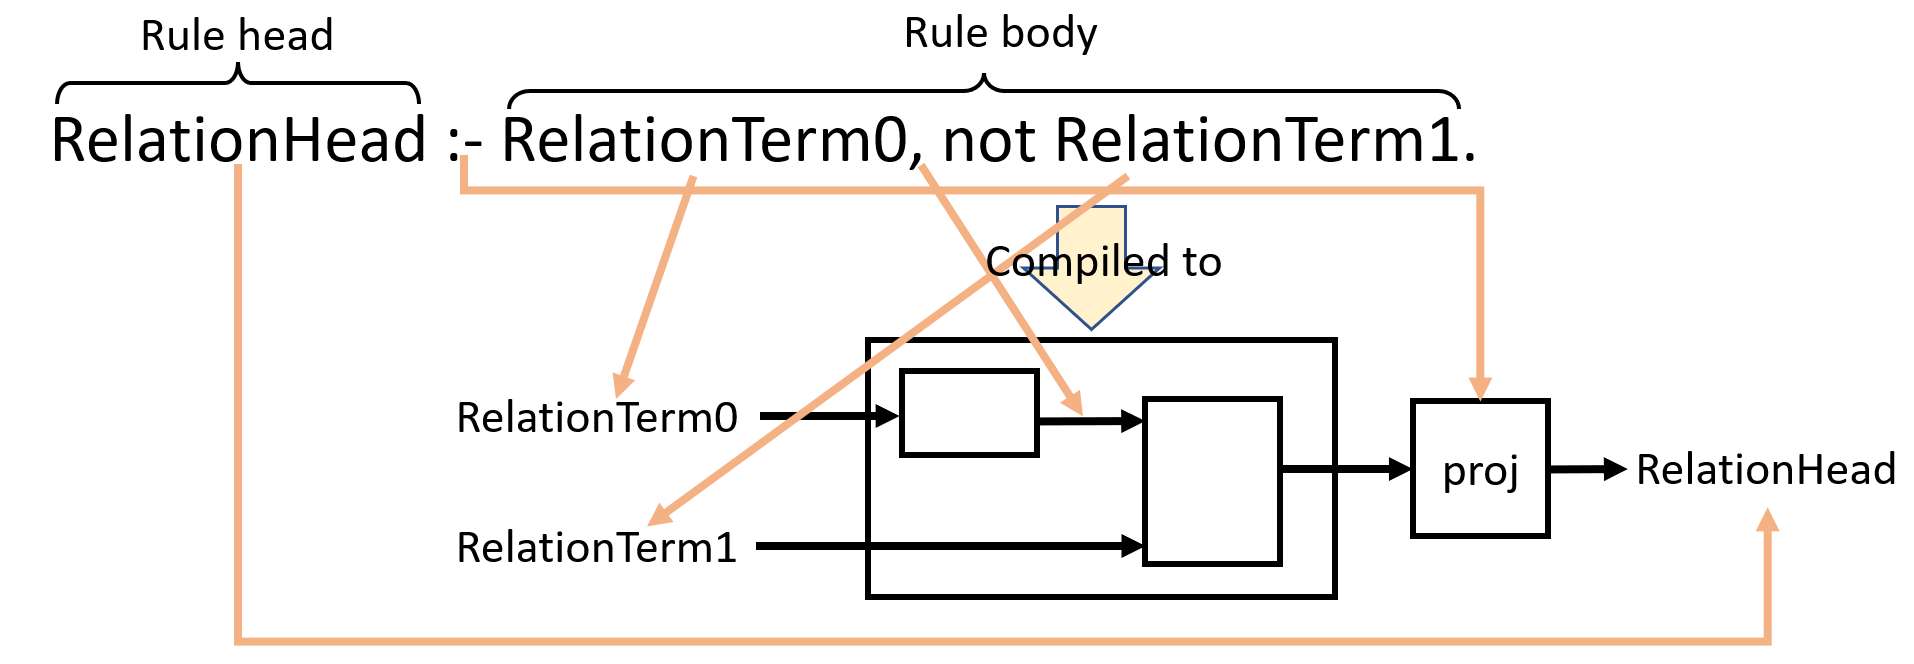
\includegraphics[width=\columnwidth,clip=true]{compilation.png}
    \caption{Compilation of a DDlog rule into a circuit.\label{fig:compilation}}
\end{figure} 

The compilation of a program containing a set of rules produces a ``toplevel'' circuit,
composed of the circuits for the rules interconnected with each other (as described
in Section~\ref{sec:connections}).
For the toplevel circuit the \code{input} relations correspond to the input 
edges.  (\code{input} relations cannot appear in the head of any rule).  Similarly,
the \code{output} relations will correspond to output edges of the toplevel circuit,
(each \code{output} relation must appear in some rule head).

\subsubsection{Relation terms in rule bodies}\label{sec:connections}

A \code{RelationTerm} is a term in a rule body containing a relation with variables substituted 
for the columns: \code{People(n, a)} is such an example.
This term \emph{defines a valuation} for all variables that appear in the columns; 
the valuation associates the variables with the contents of the relation itself.  In our example
the term \code{People(n, a)} defines the following valuation:
$(\code{n}, \code{a}) \in \{ (\code{bob}, 10), (\code{john}, 20), (\code{amy}, 10) \}$.
Each Datalog relation is represented by an edge in a circuit
carrying a \zr.  

As Figure~\ref{fig:compilation} shows, a relation in the head of a rule is compiled into the  
output edge of the circuit corresponding to the rule, and that a \code{RelationTerm}
in the body of a rule is compiled into an input edge of the circuit
corresponding to the rule.

A relation that appears in the body of a rule and in the head of another
rule is compiled into an edge connecting the circuits representing the two rules.
This is in fact just a form of function composition.

(This rule does not apply directly for recursive rules; the translation for recursive
or mutually recursive rules (which define a relation
in terms of itself), is described in Section~\ref{sec:recursion}).

For example, for the following Datalog program structure, where \code{R} is used
within a body and within a separate head:

\begin{lstlisting}[language=ddlog]
R(y) :- I(x), ....
O(y) :- ..., R(y).
\end{lstlisting}

\noindent and, given circuits $C_R$ implementing the first rule and $C_O$
implementing the second rule:

\begin{tikzpicture}[auto,>=latex]
  \node[] (I) {\code{I}};
  \node[block, right of=I] (CR) {$C_R$};
  \node[right of=CR] (R) {\code{R}};
  \draw[->] (I) -- (CR);
  \draw[->] (CR) -- (R);
  
  \node[below of=I] (RI) {\code{R}};
  \node[block, right of=RI] (CO) {$C_O$};
  \node[right of=CO] (O) {\code{O}};
  \draw[->] (RI) -- (CO);
  \draw[->] (CO) -- (O); 
\end{tikzpicture}

\noindent the translation of the program with both rules is:

\begin{tikzpicture}[auto,>=latex]
  \node[] (I) {\code{I}};
  \node[block, right of=I] (CR) {$C_R$};
  \draw[->] (I) -- (CR);
  
  \node[block, right of=R] (CO) {$C_O$};
  \node[right of=CO] (O) {\code{O}};
  \draw[->] (CR) -- node (R) {\code{R}} (CO);
  \draw[->] (CO) -- (O); 
\end{tikzpicture}

This construction is repeated for all rules, translating a program with $n$ rules into
$n$ circuits connected to each other.  If the rules are not recursive the resulting
circuit is acyclic.

\subsubsection{Repeated rule heads (set union)}\label{sec:union}\index{union}

The same relation may appear in the head of multiple rules.
In this case the contents of the head relation is the \emph{set union}
of the values assigned by all heads.
Consider the following example, where \code{I1} and \code{I2} are
rule bodies of arbitrary complexity providing a valuation for variable 
\code{v}:

\begin{lstlisting}[language=ddlog]
O(v) :- I1(v).
O(v) :- I2(v).
\end{lstlisting}

The following circuit implements the Datalog program with both rules:

\begin{tikzpicture}[auto,>=latex]
  \node[] (input1) {\code{I1}};
  \node[below of=input1, node distance=.5cm] (midway) {};
  \node[below of=midway, node distance=.5cm] (input2) {\code{I2}};
  \node[block, shape=circle, right of=midway, inner sep=0in] (plus) {$+$};
  \node[block, right of=plus, node distance=1.5cm] (distinct) {$\distinct$};
  \node[right of=distinct, node distance=1.5cm] (output) {\code{O}};
  \draw[->] (input1) -| (plus);
  \draw[->] (input2) -| (plus);
  \draw[->] (plus) -- (distinct);
  \draw[->] (distinct) -- (output);
\end{tikzpicture}

Given two \zrs $a \in \Z[I]$ and $b \in \Z[I]$
which are sets (i.e., $\isset(a)$ and $\isset(b)$), their \emph{set union} 
can be computed as: $\cup: \Z[I] \times \Z[I] \rightarrow \Z[I]$.  $a
\cup b \defn \distinct(a +_{\Z[I]} b)$.  
The $\distinct$ application is necessary to provide the set semantics of
Datalog.  We have $\isset(a) \land \isset(b) \Rightarrow
\isset(a \cup b)$ and $\ispositive(a) \land \ispositive(b)
\Rightarrow \ispositive(a \cup b)$.

Consider a concrete example for the above program where the value of \code{I1(v)} 
is $\code{v} \in \{ \code{bob} \mapsto 1, \code{mike} \mapsto 1 \}$ and the value of
\code{I2(v)} is $\code{v} \in \{ \code{bob} \mapsto 1, \code{john} \mapsto 1 \}$.
In terms of \zrs we are performing the following addition:

\noindent
\begin{tabular}{ccccc}
\begin{tabular}{|l|l|} \hline
\textbf{\code{v}} & \textbf{W} \\ \hline
\code{bob} & 1 \\
\code{mike} & 1 \\ \hline
\end{tabular} &
$+$ &
\begin{tabular}{|l|l|} \hline
\textbf{\code{v}} & \textbf{W} \\ \hline
\code{bob} & 1 \\
\code{john} & 1 \\ \hline
\end{tabular} &
$=$ &
\begin{tabular}{|l|l|} \hline
\textbf{\code{v}} & \textbf{W} \\ \hline
\code{bob} & 2 \\
\code{mike} & 1 \\
\code{john} & 1 \\ \hline
\end{tabular}
\end{tabular}

It is apparent why the $\distinct$ operator is needed.

\subsubsection{Projection}\label{sec:projection}\index{projection}

Given a valuation produced by the body of a rule, the head of
the rule defines the contents of a relation as \emph{the projection}
of the valuation on the variables used in the head.  For our example rule
\code{Names(n) :- People(n, a)}, the body defines a valuation for $(\code{n}, \code{a})$,
but the head uses only $\code{n}$.
The projection of the valuation $(\code{n}, \code{a}) \in \{ (\code{bob}, 10), (\code{john}, 20), (\code{amy}, 10) \}$
on the variable \code{n} is the valuation
$\code{n} \in \{ \code{bob}, \code{john}, \code{amy} \}$.  This defines
the contents of the relation in the head: $\code{Names} = \{ \code{bob}, \code{john}, \code{amy} \}.$

Thus, in Datalog projection is used when some of the bound variables 
in the body of a rule are not used in the head.  We can assume without loss of 
generality that a single variable is removed in a projection (by bundling multiple
variables in a single tuple-valued variable).  
Let us consider the following example, where \code{I} stands for a rule body producing
a valuation for \code{(v, v1)}.

\begin{lstlisting}[language=ddlog]
O(v) :- I(v, v1).    
\end{lstlisting}

Here the type of the implementation of \code{I} is $\Z[A_0 \times A_1]$ (a \zr of tuples with 
two elements), while the type of the implementation of \code{O} is $\Z[A_0]$.  In terms of \zrs, the
projection of a \zr $i$ on $A_0$ is defined as: $\pi_0(i)[t] = \sum_{x \in i, x|_0 = t} i[x]$, 
where $x|_0$ is first component of the tuple $x$.  The multiplicity of a tuple in the result
is the sum of the multiplicities of all tuples that project to it.

As a concrete example of projection, consider the \zr corresponding to the 
\code{People} relation and it's projection on the \code{Age} column.
The projection is $\pi_{Age}(\code{People}) = \{ 10 \mapsto 1 + 1, 20 \mapsto 1 \}$.
Notice that in the projection the weight of 10 is the sum of all weight of
the tuples that have age 10, i.e., 2.

The circuit for such a rule is:

\begin{tikzpicture}[auto,>=latex]
  \node[] (input) {\code{I}};
  \node[block, right of=input] (pi) {$\pi_0$};
  \node[block, right of=pi, node distance=1.5cm] (distinct) {$\distinct$};
  \node[right of=distinct, node distance=1.5cm] (output) {\code{O}};
  \draw[->] (input) -- (pi);
  \draw[->] (pi) -- (distinct);
  \draw[->] (distinct) -- (output);
\end{tikzpicture}

Note that $\lift{\pi}$ is time-invariant, since $\pi$ has the zero-preservation
property.  We have $\isset(i) \Rightarrow \isset(\pi_A(i))$ and $\ispositive(\pi_0)$.

\subsubsection{Flatmap in DDlog}\label{sec:flatmap} \index{flatmap} 

Recall that in DDlog the type of a column in a relation can be
any of the types supported by the language, including complex types,
such as vectors, sets, or even maps.  For example, the following
declaration indicates that the values in relation \code{I} are 
sets of integers.

\begin{lstlisting}[language=ddlog]
relation I(set: Set<integer>)
\end{lstlisting}

Flatmap is an operator that can expand the data in such a collection value
stored in a relation into the contents of a relation.  Classic Datalog does not support flatmaps. 
In DDlog \code{Flatmap} is an explicit keyword.  It appears
in rules in the form of a \code{FlatmapTerm} in 
the grammar in Figure~\ref{fig:grammar}.  The DDlog type system ensures that the \code{Flatmap} 
operator can only be applied to an expression whose type is a collection.

Here is an example of a program using \code{Flatmap}:

\begin{lstlisting}[language=ddlog]
relation I(set: Set<integer>)
relation O(integer)
O(v) :- I(set), var v = Flatmap(set).
// O = union of all sets in I
\end{lstlisting}

Each element in relation \code{I} is a set of integers.  
The DDlog \code{Flatmap}\index{\code{Flatmap}} operator implements a restricted form of
the functionality of the general mathematical operator from above 
(unlike the mathematical flatmap, which is parameterized by a function $f$, the DDlog
\code{Flatmap} uses a hardwired function, essentially the identity function.).  
The semantics is as follows: the \code{Flatmap} rule body term extends the existing valuation
with a new variable, \code{v} in this example.  \code{Flatmap}'s argument is
an expression that depends on the current valuation (\code{set} in this example)
whose value is a collection.  Let us assume that the contents of the \code{I} relation is: 
$\{ \{1,2\}, \{2,3\} \}$.  

The valuation produced by the rule \code{I(set), var v = Flatmap(set)} is
the following: $(\code{set}, \code{v}) \in  \{ (\{1,2\}, 1), (\{1,2\}, 2), 
(\{2,3\}, 2), (\{2,3\}, 3) \}$.

The circuit-based implementation of \code{Flatmap}, operating on \zrs, can be
defined as follows:

\begin{tikzpicture}[auto,>=latex]
  \node[] (input) {\code{I}};
  \node[block, right of=input, node distance=1.5cm] (map) {$\mbox{flatmap}(e)$};
  \node[block, right of=map, node distance=2cm] (distinct) {$\distinct$};
  \node[right of=distinct, node distance=1.5cm] (output) {\code{O}};
  \draw[->] (input) -- (map);
  \draw[->] (map) -- (distinct);
  \draw[->] (distinct) -- (output);
\end{tikzpicture}

\noindent where the function $e$ extends each tuple in a \zr with the newly introduced variable 
and each set value with a Cartesian product between the collection and all it's elements.
For our example: $e: \code{Set<integer>} \to \Z[\code{Set<integer>} \times \code{integer}]$ 
defined by: $e(\code{set}) = \sum_{x \in \code{set}} (\code{set}, x) \mapsto 1$.

The $\code{distinct}$ operator is needed because some collections (e.g., vectors)
may contain duplicate values.

\begin{proposition}
$\ispositive(\code{Flatmap})$.
\end{proposition}

\subsubsection{Map in DDlog}\label{sec:map}\index{map}

Given a function $f : A \rightarrow B$, the mathematical \defined{map} operator ``lifts'' the
function $f$ to operate on \zrs: $\map(f) : \Z[A] \rightarrow \Z[B]$.
map can be defined in terms of flatmap: $\map(f) \defn \mbox{flatmap}(x \mapsto 1 \cdot f(x))$.

Classic Datalog does not support map computations, but many practical
implementations do.  DDlog programs perform map computations when using \code{VariableDefinitionTerm}
in a rule, by using an expression to computing a value for a new variable, that is added to a valuation,
as in the following example:

\begin{lstlisting}[language=ddlog]
O(v) :- I(x), var v = x + 1. 
\end{lstlisting}

The \code{VariableDefinitionTerm}, \code{var v = x + 1}, extends the current valuation, which
contains just \code{x}, to include the newly defined variable \code{v}.  

The circuit implementation of the previous rule is:

\begin{tikzpicture}[auto,>=latex]
  \node[] (input) {\code{I}};
  \node[block, right of=input, node distance=1.5cm] (map) {$\mbox{map}(e)$};
  \node[right of=map, node distance=1.5cm] (output) {\code{O}};
  \draw[->] (input) -- (map);
  \draw[->] (map) -- (output);
\end{tikzpicture}

The function $e$ extends the current valuation tuple with a new column 
(corresponding to \code{v} in the example) and
evaluates the expression in the term (\code{x + 1}) for each row of the valuation
to compute the corresponding value for the new column.  In our example,
$e: \Z[\code{integer}] \to \Z[\code{integer} \times \code{integer}]$,
$e(x) = (x, x+1)$.

Note that $\ispositive(\map(f))$ for any function $f$.  
From the linearity of flatmap it follows that $\map$
is linear as well.  Moreover, the operator $\lift{\map(f)}$ is
time-invariant for any $f$.

\subsubsection{Filtering}\label{sec:filtering}

Filtering occurs in Datalog whenever a \code{TermPredicate} appears in 
the body of a rule, in the guise of a Boolean expression, as in the following example:

\noindent
\begin{lstlisting}[language=ddlog]
relation Minors(n: string, a: integer)
Minors(n, a) :- People(n, a), a < 18.
\end{lstlisting}

(A predicate may not appear in the first position in the body of a rule.)
The predicate must only use variables in the current valuation.
The produced valuation contains the same variables as the source valuation.
The value of the valuation the set of tuples in the source valuation that 
satisfy the predicate. 

Recall that the valuation of the term \code{People(n, a)} is
$(\code{n}, \code{a}) \in \{ (\code{bob}, 10), \\ (\code{john}, 20), (\code{amy}, 10) \}$.
The valuation of the entire rule is the set of tuples $(\code{n}, \code{a})$
for which the predicate $\code{a} < 18$ holds.  That valuation is
$(\code{n}, \code{a}) \in \{ (\code{bob}, 10), (\code{amy}, 10) \}$.  Thus the contents
of relation $\code{Minors}$ is $\{ (\code{bob}, 10), (\code{amy}, 10) \}$.

To compute on \zrs, let us assume that we are filtering with a predicate $P: A \rightarrow \B$.  
We define the following function $\sigma_P: A \rightarrow \Z[A]$ as:
$$\sigma_P(x) = \left\{
\begin{array}{ll}
  1 \cdot x & \mbox{ if } P(x) \\
  0 & \mbox{ otherwise } \\
\end{array}
\right.
$$

The filter of a \zr is defined as $\mbox{filter}_P: \Z[A]
\rightarrow \Z[A]$ by $\mbox{filter}_P \defn
\mbox{flatmap}(\sigma_P)$.  We have $\isset(i) \Rightarrow
\isset(\mbox{filter}_P(i))$ and $\ispositive(\mbox{filter}_P)$.  Thus a $\distinct$
is not needed.  As a consequence of the linearity of $\mbox{flatmap}$, we have
that filtering is also linear.   The lifted version of filtering is also time-invariant.

The circuit for filtering with a predicate $P$ can be implemented as:

\begin{tikzpicture}[auto,>=latex]
  \node[] (input) {\code{I}};
  \node[block, right of=input, node distance=2cm] (map) {$\mbox{flatmap}(\sigma_P)$};
  \node[right of=map, node distance=2cm] (output) {\code{O}};
  \draw[->] (input) -- (map);
  \draw[->] (map) -- (output);
\end{tikzpicture}

\subsubsection{Grouping}\index{grouping}\label{sec:grouping}

Classic Datalog does not support grouping.
In DDlog grouping is the fundamental operator used for aggregation.  
Grouping is applied to a set and produces a partition of that set
into a set of collections.  The type of a partition is a built-in
type in DDlog, called \code{Group}.
The following example shows an example of grouping in DDlog:

\begin{lstlisting}[language=ddlog]
output relation O(v: Group<integer, string>) 
// Groups with key integer and values Vector<string>
ByAge(g) :- People(n, a), var g = (n).group_by(a).  
// Each g is the group of all names that have the same age
\end{lstlisting}

The general syntax of a \code{GroupByTerm} in Figure~\ref{fig:grammar} is given by: \\
\code{var g = (project-expression).group\_by(key-expression)}.
In DDlog the \code{key-expression} is restricted to be a tuple 
of variables in the current valuation.

The semantics of a \code{GroupByTerm} is given by the following algorithm:

\begin{enumerate}
    \item We start with some input valuation.
    \item The \code{project-expression} is evaluated for the input valuation $V$,
    adding a new (anonymous) variable to the valuation, storing the result
    of the \code{project-expression} for each row.
    \item The resulting valuation is projected on a tuple of variables containing
    the new anonymous variable and all variables that appear in \code{key-expression}.
    The result of the projection is a new valuation $P$, a set (with no duplicates).
    This valuation \emph{only includes the variables that appear in the projection and
    the key expression}; all other variables are removed.  This behavior is unusual --- 
    this is the only DDlog operator that removes variables from a valuation.
    \item Finally, the data in the valuation is grouped by key,
    and the result is a valuation that contains for the new variable a group.
\end{enumerate}

As an example, let us evaluate the above DDlog rule according to these steps:

\begin{enumerate}
    \item The term \code{Persons(n, a)} provides the following valuation: \\
    $(\code{n},\code{a}) \in \{ (\code{bob}, 10), (\code{john}, 20), (\code{amy}, 10) \}$.
    \item In our example \code{project-expression} is just \code{n}, whose value
    will be assigned to the anonymous variable.  This creates a new valuation: \\
    $(\code{n},\code{a}, \code{anonymous}) \in \{ (\code{bob}, 10, \code{bob}), 
    (\code{john}, 20, \code{john}),  (\code{amy}, 10, \code{amy}) \}$.
    \item The valuation is projected on \code{a} (the group key) and \code{anonymous}
    (the projection key), obtaining:
    $(\code{a}, \code{anonymous}) \in \{ (10, \code{bob}), (20, \code{john}),  (10, \code{amy}) \}$.
    In this case there are no duplicates, but any duplicates would be removed.
    \item The values in the valuation are grouped by their \code{a} value, providing
    a new group for each value.  The variable \code{g} is added to the resulting valuation.
    The result is $(\code{a}, \code{g}) \in \{ (10, [\code{bob}, \code{amy}]), (20, [\code{john}]) \}$.
    Notice how the value of \code{g} in the valuation is a collection, shown with square brackets.
\end{enumerate}

Let us define this computation in terms of \zrs.  Consider an arbitrary type of 
keys $K$, and a function that computes a key for a value $k: I \rightarrow K$.  
Then we define $\mbox{groupby}(k): \Z[I] \rightarrow \Z[I][K]$, as
$\mbox{groupby}(k)(i) = \sum_{x \in i} \{ k(x) \mapsto 1 \cdot x \}$.
Note that groupby always produces a set of \zrs.  The weight of each group
is always 1.  Note that $\ispositive(\mbox{groupby}(k))$.  Also, $\lift{\mbox{groupby}(k)}$
is time-invariant for any function $k$, since $\mbox{groupby}(k)$ has the zero-preservation
property.
 
The implementation of the \code{group\_by} operator requires chaining the implementation of the
projection and of groupby function just described:
the resulting circuit is (using $p$ as the translation of \code{project-expression} and $k$ as
the translation of \code{key-expression}):

\begin{tikzpicture}[auto,>=latex]
  \node[] (input) {\code{I}};
  \node[block, right of=input, node distance=1.5cm] (map) {$map(p)$};
  \node[block, right of=map, node distance=1.5cm] (pi) {$\pi_{anon,k}$};
  \node[block, right of=pi, node distance=2cm] (distinct) {$\distinct$};
  \node[block, right of=distinct, node distance=2cm] (group) {groupby($k$)};
  \node[right of=group, node distance=2cm] (output) {\code{O}};
  \draw[->] (input) -- (map);
  \draw[->] (map) -- (pi);
  \draw[->] (pi) -- (distinct);
  \draw[->] (distinct) -- (group);
  \draw[->] (group) -- (output);
\end{tikzpicture}

\subsubsection{Aggregation}\label{sec:aggregation}  

Classic Datalog does not support aggregations
but many practical implementations have extended Datalog with
a construct equivalent with a composition of groupby-aggregate. 

Strictly speaking, DDlog does not support for aggregation -- the only
aggregate supported is a group.  However, since DDlog allows users to apply arbitrary
functions to a \code{Group} object, traditional aggregation can be performed
by grouping and then applying a scalar-returning function using a \code{map}, as described
Section~\ref{sec:map}.  Consider the following example, an extension of 
the example in Section~\ref{sec:grouping}:

\begin{lstlisting}[language=ddlog]
output relation NamesByAge(s: string) 
NamesByAge(s) :- ByAge(g), 
      var s = g.key + ": " + g.toString().  
\end{lstlisting}

This example uses built-in functions \code{g.key} that obtains the key of a group, 
and \code{g.toString()}, which converts the group contents to a string.

Formally, given a function $a: \code{Group<$K$,$I$>} \to O$, 
aggregation is just $\map(a)$ applied to a set of groups.  As a consequence
lifted aggregation is time-invariant.

\subsubsection{Cartesian products}\label{sec:cartesian}

Cartesian products in Datalog appear from the use of in a rule body of a \code{TermRelation} 
where the relation arguments are all new variables (not already defined in the input valuation).  
The Datalog semantics of Cartesian products is to produce a new valuation that includes all
variables, and having as values the Cartesian product of the values of the input
valuation and the relation in the term.

The following program shows an example Cartesian product:

\begin{lstlisting}[language=ddlog]
O(v1, v2) :- I1(v1), I2(v2).
\end{lstlisting}

A Cartesian product is implemented as a circuit using the product operation on \zrs.
For $i_1 \in \Z[A]$ and $i_2 \in \Z[B]$ we define $i_1 \times i_2 \in \Z[A \times B]$ by
$(i_1 \times i_2)(\pair{x}{y}) \defn i_1[x] \times i_2[y] . \forall x \in i_1, y \in i_2$.
The circuit computing the Cartesian product is given by:

\begin{tikzpicture}[auto,>=latex]
  \node[] (i1) {\code{I1}};
  \node[below of=i1, node distance=.5cm] (midway) {};
  \node[below of=midway, node distance=.5cm] (i2) {\code{I2}};
  \node[block, right of=midway] (prod) {$\lift{\times}$};
  \node[right of=prod] (output) {\code{O}};
  \draw[->] (i1) -| (prod);
  \draw[->] (i2) -| (prod);
  \draw[->] (prod) -- (output);
\end{tikzpicture}

As an example, let us consider the product of the following two \zrs:

\noindent
\begin{tabular}{ccccc}
\begin{tabular}{|l|l|} \hline
\textbf{\code{x}} & \textbf{W} \\ \hline
\code{bob} & 1 \\
\code{mike} & 2 \\ \hline
\end{tabular} &
$\times$ &
\begin{tabular}{|l|l|} \hline
\textbf{\code{y}} & \textbf{W} \\ \hline
\code{bob} & 1 \\
\code{john} & -1 \\ \hline
\end{tabular} &
$=$ &
\begin{tabular}{|l|l|} \hline
\textbf{(\code{x}, \code{y})} & \textbf{W} \\ \hline
$(\code{bob}, \code{bob})$ & 1 \\
$(\code{mike}, \code{bob})$ & 2 \\
$(\code{bob}, \code{john})$ & -1 \\
$(\code{mike}, \code{john})$ & -2 \\ \hline
\end{tabular}
\end{tabular}

Notice that $\isset(x) \land \isset(y) \Rightarrow \isset(x \times y)$.
The Cartesian product as defined on \zrs is a bilinear operator.  Also,
$\lift{\times}$ is time-invariant.

\subsubsection{Joins}\label{sec:join}

A join appears in a Datalog program by using a \code{TermRelation}
that has as arguments some variables that are already defined in the current valuation.
The following example shows a join: since the second relation reuses variable \code{v},
which is already bound by the valuation, this is a join, and not a Cartesian product:

\begin{lstlisting}[language=ddlog]
O(x, y) :- I1(x, v), I2(v, y).
\end{lstlisting}

The semantics of a join can be modeled as a cartesian product followed by a sequence of filters.
This is achieved by using fresh variable names for the arguments of each 
\code{TermRelation}, and adding predicates that require these fresh variables
to be equal to the bound variables they replace.
For example, the following program is equivalent to the one above.

\begin{lstlisting}[language=ddlog]
O(x, y) :- I1(x, v), I2(v1, y), v = v1.
\end{lstlisting}

Since a join is a composition of a bilinear (the Cartesian product) and a linear (filtering) operator, it is also a bilinear operator, and thus its lifted version is time-invariant.

In practice joins are very important computationally, and they are
implemented by a custom operator on \zrs denoted by $\bowtie$.

The circuit computing the join product is given by:

\begin{tikzpicture}[auto,>=latex]
  \node[] (i1) {\code{I1}};
  \node[below of=i1, node distance=.5cm] (midway) {};
  \node[below of=midway, node distance=.5cm] (i2) {\code{I2}};
  \node[block, right of=midway] (prod) {$\bowtie$};
  \node[right of=prod] (output) {\code{O}};
  \draw[->] (i1) -| (prod);
  \draw[->] (i2) -| (prod);
  \draw[->] (prod) -- (output);
\end{tikzpicture}

\subsubsection{Set intersection}\label{sec:intersection}

Set intersection in Datalog is just a particular case of join where a \code{TermRelation}
uses \emph{all} the variables defined in the current valuation as arguments.
In the following example relation \code{O} is the 
intersection of relations \code{I1} and \code{I2}:

\begin{lstlisting}[language=ddlog]
O(v) = I1(v), I2(v).
\end{lstlisting}

The join implementation using circuits immediately applies to set intersections.
It follows that set intersection is a bilinear operator, and thus time-invariant 
when lifted.

\subsubsection{Negation}\label{sec:negation}\index{negation}

We only support Datalog programs with stratified negation.  
See~\cite{Abiteboul-book95} for a precise definition.  
Negation in a Datalog program is introduced syntactically by a \code{NegatedTerm} 
from the grammar in Figure~\ref{fig:grammar}.  A negated term
cannot appear first in a rule body.  All variables that
appear in the negated term must have been already defined
by previous terms in the body.  

With these syntactic constraints the are two different meanings to 
negation:

\begin{itemize}
    \item If the negated term uses \emph{all} variables already in the valuation, 
    it is modeled as a set difference.
    \item If the negated term uses a subset of all the variables in the
    existing valuation, it is modeled as an antijoin.
\end{itemize}

We describe each of these two cases.

\subsubsection{Set difference}\index{set difference}\label{sec:set-difference}

If the \code{NegatedTerm} contains as arguments all variables in the current valuation,
the meaning of negation is just set difference: the resulting valuation
will \emph{exclude} all tuples from the negated relation.

For example, consider the rule:

\begin{lstlisting}[language=ddlog]
relation Major(name: string, age: integer)
Major(n, a) :- People(n, a), not Minor(n, a).
\end{lstlisting}

The valuation computed by the rule's body is $\{ (\code{bob}, 10), (\code{john}, 20), (\code{amy}, 10) \} 
\setminus \{ (\code{bob}, 10), (\code{amy}, 10) \} = \{ (\code{john}, 20) \}$.

In terms of \zrs, let us consider the following program:

\begin{lstlisting}[language=ddlog]
O(v) :- I1(v), not I2(v).     
\end{lstlisting}

We define the set difference on \zrs as follows: 
$\setminus: \Z[I] \times \Z[I] \rightarrow \Z[I]$, where $i_1
\setminus i_2 = \distinct(i_1 - i_2)$.  Note
that we have $\forall i_1, i_2, \ispositive(i_1 \setminus
i_2)$ due to the application of the $\distinct$ operator.

The circuit computing the valuation of the body of this rule is:

\begin{tikzpicture}[auto,>=latex]
  \node[] (i1) {\code{I1}};
  \node[below of=i1, node distance=.5cm] (midway) {};
  \node[below of=midway, node distance=.5cm] (i2) {\code{I2}};
  \node[block, shape=circle, inner sep=0in, right of=i2] (m) {$-$};
  \node[block, right of=midway, shape=circle, inner sep=0in, node distance=2cm] (plus) {$+$};
  \node[block, right of=plus, node distance=1.5cm] (distinct) {$\distinct$};
  \node[right of=distinct, node distance=1.5cm] (output) {\code{O}};
  \draw[->] (i1) -| (plus);
  \draw[->] (i2) -- (m);
  \draw[->] (m) -| (plus);
  \draw[->] (plus) -- (distinct);
  \draw[->] (distinct) -- (output);
\end{tikzpicture}

This whole circuit is time-invariant, since it composed only of
time-invariant operators.

\subsubsection{Antijoin}\label{sec:antijoin}\index{antijoin}

Antijoin is the semantics of a Datalog \code{NegatedTerm} that uses a relation
which does not use some of the variables in the current valuation.
Consider the following program:

\begin{lstlisting}[language=ddlog]
O(v) :- I1(v, z), not I2(v).     
\end{lstlisting}

The semantics of such a rule can be defined in terms of joins and set difference.
This rule is equivalent with the following pair of rules:

\begin{lstlisting}[language=ddlog]
C(v, z) :- I1(v, z), I2(v).
O(v) :- I1(v, z), not C(v, z).     
\end{lstlisting}

This transformation reduces an antijoin to a join (using all variables in the current valuation), 
followed by a set difference.  The translation of these rules is covered by Sections~\ref{sec:join} and
Section~\ref{sec:set-difference}.  In terms of circuits we can just build the circuit 
for the pair of rules:

\begin{tikzpicture}[auto,>=latex]
  \node[] (i1) {\code{I1}};
  \node[below of=i1, node distance=.5cm] (i2) {\code{I2}};
  \node[block, right of=i1, node distance=1.5cm] (join) {$\bowtie$};
  \node[block, shape=circle, inner sep=0in, right of=join] (m) {$-$};
  \node[block, above of=m, shape=circle, inner sep=0in, node distance=.6cm] (plus) {$+$};
  \node[block, right of=plus, node distance=1.5cm] (distinct) {$\distinct$};
  \node[right of=distinct, node distance=1.5cm] (output) {\code{O}};
  \draw[->] (i1) -- node (tap) {} (join);
  \draw[->] (i2) -| (join);
  \draw[->] (join) -- (m);
  \draw[->] (m) -- (plus);
  \draw[->] (tap.south) |- (plus);
  \draw[->] (plus) -- (distinct);
  \draw[->] (distinct) -- (output);
\end{tikzpicture}

\subsection{Streaming Differential Datalog}\label{sec:ddlog}

In this section we have shown how Given a Datalog (or SQL) query $Q$, 
can be converted into a circuit $C_Q$ that computes the same input-output function as $Q$.  

\begin{tikzpicture}[auto,node distance=1cm,>=latex]
    \node[] (input) {$i$};
    \node[block, right of=input] (q) {$C_Q$};
    \node[right of=q] (output) {$o$};
    \draw[->] (input) -- (q);
    \draw[->] (q) -- (output);
\end{tikzpicture}

We can perform two simple transformations to this circuit: we can lift it to convert it
into a streaming program, and then we can incrementalize it, to convert it into a
differential program.

\subsubsection{Streaming Datalog}

Given the circuit $C_Q: A \to B$, We can lift it to compute on \emph{streams} 
of relations.  $\lift{C_Q}: \stream{A} \to \stream{B}$ interacts with its environment 
in ``epochs,'' corresponding to the time dimension of the streams.  In each epoch the circuit
receives a new set of values for the inputs relations and it provides the corresponding values
for the output relations.

\begin{tikzpicture}[auto,node distance=1cm,>=latex]
    \node[] (input) {$i$};
    \node[block, right of=input] (q) {$\lift{C_Q}$};
    \node[right of=q] (output) {$o$};
    \draw[->] (input) -- (q);
    \draw[->] (q) -- (output);
\end{tikzpicture}

\subsubsection{Streaming Differential Datalog}

Furthermore, we can apply the $\inc{\cdot}$ operator to the streaming circuit $\lift{C_Q}$, 
converting it into an incremental streaming circuit: $\inc{(\lift{C_Q})}: \stream{A} \to \stream{B}$.

\begin{tikzpicture}[auto,node distance=1cm,>=latex]
    \node[] (input) {$i$};
    \node[block, right of=input] (I) {$\I$};
    \node[block, right of=I] (q) {$\lift{C_Q}$};
    \node[block, right of=q] (D) {$\D$};
    \node[right of=D] (output) {$o$};
    \draw[->] (input) -- (I);
    \draw[->] (I) -- (q);
    \draw[->] (q) -- (D);
    \draw[->] (D) -- (output);
\end{tikzpicture}

This is a differential streaming version of the circuit $C_Q$.  This circuit
interacts with its environment in ``ephochs,'' corresponding to the time dimension of the streams.  
In each epoch the circuit receives a new set of \emph{changes} to the inputs relations and it
provides the corresponding \emph{change} for the output relations.

This is in essence the service provided by the DDlog compiler: given a query $Q$
it provides a streaming implementation of $\inc{\lift{C_Q}}$.  However, the DDlog
runtime provides some additional services, described in the next section.


\section{Implementation}\label{sec:implementation}

We are prototyping an implementation of \dbsp as part of an
open-source project with an MIT license: 
\url{https://github.com/vmware/database-stream-processor}.
The implementation is written in Rust.
The implementation consists of a library and a runtime.
The library provides APIs for basic algebraic data types:
such as groups, finite maps, \zr, indexed \zr.  
A separate circuit construction API allows users to 
create \dbsp circuits by placing operator nodes (corresponding to boxes in our diagrams)
and connecting them with streams, which correspond to the
arrows in our diagrams.  The library provides pre-built generic operators
for integration, differentiation, delay, nested integration and differentiation.
The \zr library provides functions for computing the basic \zr operations
corresponding to plus, negation, grouping, joining, aggregation.

For iterative computations we provide the $\delta_0$ operator and
an operator that approximates $\int$ by terminating iteration of
a loop at a user-specified condition (usually the condition is the 
requirement for a zero to appear in a specified stream).
The low level library allows users to construct incremental
circuits manually.  Our plan is to add a higher-level library
(a compiler) which will automatically incrementalize a circuit.

\section{Additional Implementation Details}\label{sec:implementation-additional}

\subsection{Checkpoint/restore}

DDlog programs are stateful streaming systems.  Fault-tolerance and 
migration for such programs requires state migration.  We claim that it is 
sufficient to checkpoint and restore the "contents" of all $\zm$ operator
in order to migrate the state of a Ddlog computation.

\subsection{Maintaining a database}

DDlog is not a database, it is just a streaming view maintenance system.
In particular, DDlog will not maintain more state than absolutely necessary
to compute the changes to the views.  There is no way to find out whether 
a specific value exists at a specific time moment within a DDlog relation.
However, a simple extension to DDlog runtime can be made to provide a \emph{view query}
API: essentially all relations that may be queried have to be maintained 
internally in an integrated form as well.  The system can then provide
an API to enumerate or query a view about element membership between 
input updates.

\subsection{Materialized views}

An incremental view maintenance system is not a database -- it only computes changes
to views when given changes to tables.  However, it can be integrated with a 
database, by providing capabilities for \emph{querying} both tables and views.
An input table is just the integral of all the changes to the table.  This makes
possible building a system that is both stateful (like a database) and streaming
(like an incremental view maintenance system).

\subsection{Maintaining input invariants}

For relational query systems there is however an important caveat: 
the proofs about the correctness
of the $C_Q$ implementing the same semantics as $Q$ all require some 
preconditions on the circuit inputs.  In particular, the semantics of $Q$
is only defined for sets.  In order for $C_Q$ to faithfully emulate
the behavior of $Q$ we must enforce the invariant that the input
relations are in fact sets.  

However, the differential streaming version of the circuits accepts
an arbitrary stream of changes to the input relations.  Not all
such streams define input relations that are sets!  For example,
consider an input stream where the first element removes a
tuple from an input relation.  The resulting \zr does not represent
a set, and thus the proof of correctness does not hold.
This problem has been well understood in the context of the
relational algebra: it is the same as the notion of positivity from~\cite{green-tcs11}.

We propose three different solutions to this problem, in increasing degrees of complexity.

\paragraph{Assume that the environment is well-behaved}

The simplest solution is to do nothing and assume that at any point in time 
the integral of the input stream of changes $i$ is a set: $\forall t \in \N . \isset(\I(i)[t])$.
This may be a reasonable assumption if the changes come from a controlled
medium, e.g., a traditional database, where they represent legal database changes.

\paragraph{Normalize input relations to sets}

In order to enforce that the input relations are always sets it is sufficient
to apply a $\distinct$ operator after integration.  

\begin{tikzpicture}[auto,node distance=1cm,>=latex]
    \node[] (input) {$i$};
    \node[block, right of=input] (I) {$\I$};
    \node[block, right of=I, node distance=1.5cm] (distinct) {$\distinct$};
    \node[block, right of=distinct, node distance=1.5cm] (q) {$\lift{C_Q}$};
    \node[block, right of=q] (D) {$\D$};
    \node[right of=D] (output) {$o$};
    \draw[->] (input) -- (I);
    \draw[->] (I) -- (distinct);
    \draw[->] (distinct) -- (q);
    \draw[->] (q) -- (D);
    \draw[->] (D) -- (output);
\end{tikzpicture}

The semantics of the resulting circuit is identical to the semantics of $\inc{\lift{C_Q}}$
for well-behaved input streams.  For non-well behaved input streams one can give
a reasonable definition: a change is applied to the input relations, and then non-relations
are normalized into relations.  Removing a non-existent element is a no-op, and adding twice
an element is the same as adding it once.

\paragraph{Use a ``change manager''}

In this solution we interpose a separate software component between the environment
and the circuit.  Let us call this a ``change manager'' (CM).  The CM
is responsible for accepting commands from the environment that perform updates on the input
relations, validating them, and building incrementally an input change, by computing the
effect of the commands.  The CM needs to maintain enough internal state to validate all commands; this 
will most likely entail maintaining the full contents of the input tables.  Note that
the input tables can be computed as the $\I$ of all input deltas ever applied.  Once all 
commands producing a change have been accepted, the environment can apply the produced input change
atomically, and obtain from the circuit the corresponding output changes.

\begin{tikzpicture}[auto,node distance=1cm,>=latex]
    \node[minimum width=.5cm, minimum height=1cm] (env) {Env};
    \node[block, right of=env, minimum width=.5cm, minimum height=1cm, node distance=1.5cm] (tm) {CM};
    \node[block, right of=tm, node distance=1.5cm] (C) {$\inc{\lift{C_Q}}$};
    \node[right of=C] (output) {$o$};
    \draw[->] (env.30) -- (tm.150);
    \draw[<-] (env.330) -- (tm.210);
    \draw[->] (tm) -- node (i) {$i$} (C);
    \draw[->] (C) -- (output);
\end{tikzpicture}

\part{Appendixes}
\appendix
\section{Z-transform and stream convolutions}\label{sec:ztransform}

\begin{definition}
The \defined{Z-transform} of a stream, as traditionally defined in signal processing, 
is a function that associates with any stream over a group a formal power series in the 
indeterminate $z$: $\mathcal{Z}: \stream{A} 
\rightarrow A\llbracket z \rrbracket$ defined as $\mathcal{Z}(s) \defn \sum_{t \geq 0} s[t] z^{-t}$. 
\end{definition}

For example, the Z-transform of the $\id$ stream is the power series 
$0 + \zm + z^{-2} + z^{-3} + \ldots$.

\begin{definition}
Let $(R,+,\cdot,0,1)$ be a commutative ring.
The \defined{Cauchy product} (also called discrete convolution) of two streams 
$\ast : \stream{R} \times \stream{R} \rightarrow \stream{R}$  is defined as:
$$
(a\ast b)[t] ~=~ \sum_{i=0}^t a[i]\cdot b[t-i]
$$
\end{definition}

For example, the convolution of the $\id$ stream with itself is the
stream $\id \ast \id$ containing the sequence of values 
$0, (0 \cdot 1 + 1 \cdot 0), (0 \cdot 2 + 1 \cdot 1 + 2 \cdot 0), \ldots =
0, 0, 1, 4, 8, \ldots$.

\begin{proposition}
The structure $(\stream{R},+,\ast,0,1)$ 
is also a commutative ring. This ring is isomorphic to the ring of
formal power series in one indeterminate $R\llbracket z \rrbracket$ with coefficients from $R$.
\end{proposition}


Sometimes it is more convenient to use the formal power series notation.
Notice that we have $\zm(s) = \zm \ast s$, 
justifying the traditional notation for the delay operator $\zm$.
It follows that the differentiation of a stream 
$s$ is $\D(s)=(1-\zm)\ast s$. 

Moreover, the equation that defines the integration of a stream $s$, $\xi=\zm(\xi)+s$ is equivalent
to $\xi=\zm\ast\xi + s$ and then to $(1-\zm)\ast\xi=s$. Since $1-\zm$ has multiplicative inverse
$$
(1-\zm)^{-1} ~=~ 1+\zm+z^{-2}+z^{-3}+\cdots
$$
we can express the integration operator by $\I(s) = (1-\zm)^{-1}\ast s$. Theorem~\ref{inverses} now
follows by algebraic manipulations in the ring of formal power series. Similarly for the time-invariance
and linearity properties of $\D$ and $\I$. Even causality can be treated algebraically, once we note that,
like addition, convolution is causal.

\paragraph{Observation} As shown above, there are two proof styles
for equations over streams: one is (usually) by induction over the
time dimension,
and the other one is equational, by operating with
polynomials over $z$.  The theory of digital signal processing posits
that these two proof styles give the same results.


\printindex

\bibliographystyle{plainurl}
\bibliography{main}

\end{document}
